% =====================================================================
%  Mathematical Tools for Fluid Mechanics -- A Study & Review Guide
%  Companion to Appendix B of Kundu, Cohen & Dowling, Fluid Mechanics (6th ed., 2016)
%  with exercises, Python checks, and connections to Earth-surface dynamics
%
%  Compile with pdfLaTeX (Overleaf default). Compile twice for cross-references.
% =====================================================================
\documentclass[11pt,letterpaper]{article}

% ------------------------- USER SWITCHES -----------------------------
\newif\ifshowsolutions
\showsolutionstrue      % change to \showsolutionsfalse for a problems-only version
% ---------------------------------------------------------------------

% ------------------------- Fonts & layout ----------------------------
\usepackage[T1]{fontenc}
\usepackage[utf8]{inputenc}
\usepackage{lmodern}            % scalable fonts (used for typewriter/code)
\usepackage[sc]{mathpazo}       % Palatino text + math (close to Kundu's typeface)
\linespread{1.05}
\usepackage{microtype}
\usepackage[letterpaper,margin=1in,headheight=14pt]{geometry}
\setlength{\parindent}{0pt}
\setlength{\parskip}{0.55em}

% ------------------------- Mathematics -------------------------------
\usepackage{amsmath,amssymb,mathtools}
\usepackage{bm}
\numberwithin{equation}{section}
\allowdisplaybreaks[2]

% ------------------------- Utilities ---------------------------------
\usepackage{etoolbox}
\usepackage[dvipsnames]{xcolor}
\definecolor{keyblue}{HTML}{1F4E8C}
\definecolor{pitred}{HTML}{B22222}
\definecolor{resgreen}{HTML}{2E7D4F}
\definecolor{exorange}{HTML}{C0661A}
\definecolor{pygray}{HTML}{4D4D4D}
\definecolor{srcpurple}{HTML}{6A4C93}
\definecolor{quizamber}{HTML}{B7791F}

\usepackage{graphicx}
\usepackage{booktabs,array,tabularx,multirow}
\usepackage[shortlabels]{enumitem}
\setlist{itemsep=2pt,topsep=3pt,parsep=0pt}
\usepackage{caption}
\captionsetup{font=small,labelfont=bf,margin=10pt}
\usepackage{titlesec}
\usepackage{fancyhdr}
\usepackage{multicol}

% ------------------------- Graphics ----------------------------------
\usepackage{tikz}
\usetikzlibrary{arrows.meta,calc,decorations.markings,patterns,positioning}
\usepackage{tikz-3dplot}
\usepackage{pgfplots}
\pgfplotsset{compat=1.18}
% erf(x) is not built into pgfplots; this odd, smooth approximation has |error| < 4e-4
\tikzset{declare function={erfa(\x)=tanh(1.1283791671*(\x+0.0894309*\x^3));}}

% ------------------------- Boxes & code ------------------------------
\usepackage[most]{tcolorbox}
\usepackage{listings}

% ------------------------- References & links ------------------------
\usepackage[round,sort]{natbib}
\usepackage[colorlinks=true,linkcolor=keyblue,citecolor=resgreen,urlcolor=srcpurple,
            bookmarksnumbered=true,pdfusetitle,hypertexnames=false]{hyperref}
\usepackage[capitalise,noabbrev,nameinlink]{cleveref}

% ------------------------- Headings & headers ------------------------
\titleformat{\section}{\Large\bfseries\color{keyblue}}{\thesection}{0.8em}{}[{\color{keyblue!35}\titlerule[0.8pt]}]
\titleformat{\subsection}{\large\bfseries\color{keyblue!85!black}}{\thesubsection}{0.7em}{}
\titleformat{\subsubsection}{\normalsize\bfseries}{\thesubsubsection}{0.6em}{}
\titlespacing*{\section}{0pt}{2.0ex plus 1ex minus .2ex}{1.2ex}
\titlespacing*{\subsection}{0pt}{1.6ex plus 1ex minus .2ex}{0.6ex}

\pagestyle{fancy}
\fancyhf{}
\fancyhead[L]{\small\color{gray}Mathematical Tools -- Study Guide}
\fancyhead[R]{\small\color{gray}\nouppercase{\leftmark}}
\fancyfoot[C]{\small\thepage}
\renewcommand{\headrulewidth}{0.3pt}

% ------------------------- Math macros -------------------------------
\newcommand{\uu}{\mathbf{u}}
\newcommand{\xx}{\mathbf{x}}
\newcommand{\XX}{\mathbf{X}}
\newcommand{\nn}{\mathbf{n}}
\newcommand{\FF}{\mathbf{F}}
\newcommand{\qq}{\mathbf{q}}
\newcommand{\tv}{\mathbf{t}}
\newcommand{\e}[1]{\mathbf{e}_{#1}}
\newcommand{\bomega}{\bm{\omega}}
\newcommand{\pd}[2]{\frac{\partial #1}{\partial #2}}
\newcommand{\pdd}[2]{\frac{\partial^2 #1}{\partial #2^2}}
\newcommand{\pdm}[3]{\frac{\partial^2 #1}{\partial #2\,\partial #3}}
\newcommand{\od}[2]{\frac{d #1}{d #2}}
\newcommand{\Dt}[1]{\frac{D #1}{Dt}}
\newcommand{\units}[1]{\,\mathrm{#1}}
\DeclareMathOperator{\erf}{erf}
\DeclareMathOperator{\sgn}{sgn}
\newcommand{\Kundu}{\textnormal{\textsc{kcd}}}   % Kundu, Cohen & Dowling (2016)

% ------------------------- Box styles --------------------------------
\tcbset{
  guidebox/.style={enhanced,breakable,arc=2pt,boxrule=0.6pt,left=6pt,right=6pt,top=4pt,bottom=4pt,
                   fonttitle=\bfseries\small,before skip=9pt,after skip=9pt},
}
\newtcolorbox{keyidea}[1][]{guidebox,colback=keyblue!5,colframe=keyblue!85!black,
  title={Key idea\ifstrempty{#1}{}{: #1}}}
\newtcolorbox{pitfall}[1][]{guidebox,colback=pitred!4,colframe=pitred!85!black,
  title={Common pitfall\ifstrempty{#1}{}{: #1}}}
\newtcolorbox{research}[1][]{guidebox,colback=resgreen!5,colframe=resgreen!85!black,
  title={Research connection\ifstrempty{#1}{}{: #1}}}
\newtcolorbox[auto counter,number within=section]{worked}[1][]{guidebox,colback=white,
  colframe=keyblue!60!black,colbacktitle=keyblue!12,coltitle=black,
  title={Worked example~\thetcbcounter\ifstrempty{#1}{}{: #1}}}
\newtcolorbox{remember}{guidebox,colback=gray!6,colframe=gray!55!black,title={What to remember}}
\newtcolorbox{goals}{guidebox,colback=white,colframe=keyblue!40,coltitle=keyblue!80!black,
  colbacktitle=keyblue!8,title={Learning goals}}
\newtcolorbox{source}{enhanced,breakable,sharp corners,boxrule=0pt,frame hidden,
  colback=srcpurple!6,borderline west={3pt}{0pt}{srcpurple},fontupper=\small,
  left=8pt,right=6pt,top=3pt,bottom=3pt,before skip=4pt,after skip=10pt}
\newtcolorbox{quizbox}[1][]{guidebox,colback=quizamber!5,colframe=quizamber!90!black,
  title={#1}}

% Exercises: \begin{exercise}[Title]{level 1-3}{key} ... \end{exercise}
\newcommand{\lvl}[1]{\ifcase#1\or$\star$\or$\star\star$\or$\star\star\star$\fi}
\newtcolorbox[auto counter,number within=section]{exercise}[3][]{guidebox,unbreakable,
  colback=exorange!3,colframe=exorange!85!black,
  title={Exercise~\thetcbcounter\enspace\lvl{#2}\ifstrempty{#1}{}{\enspace #1}%
    \ifshowsolutions\hfill\hyperref[sol:#3]{\normalfont\small\color{white}solution\,$\blacktriangleright$}\fi},
  label={ex:#3}}

% Solutions (collected in the appendix)
\newenvironment{solution}[1]{%
  \par\addvspace{1.0ex}\noindent\phantomsection\label{sol:#1}%
  {\color{exorange!85!black}\bfseries Solution to Exercise~\ref{ex:#1}}%
  \hfill\hyperref[ex:#1]{\small$\blacktriangleleft$\,back to exercise}\par\nopagebreak\smallskip}%
  {\par\smallskip\noindent{\color{exorange!40}\rule{\linewidth}{0.4pt}}\par}

% Python listings
\lstdefinestyle{py}{language=Python,basicstyle=\ttfamily\footnotesize,
  keywordstyle=\color{keyblue}\bfseries,commentstyle=\color{resgreen!75!black}\itshape,
  stringstyle=\color{pitred!80!black},showstringspaces=false,columns=fullflexible,
  keepspaces=true,breaklines=true,upquote=true,tabsize=4}
\newtcblisting{pycode}[1][]{guidebox,unbreakable,listing only,colback=pygray!4,colframe=pygray!85!black,
  title={Python check\ifstrempty{#1}{}{: #1}},listing options={style=py}}

% Tag for equations quoted from Kundu, Cohen & Dowling Appendix B
\newcommand{\ktag}[1]{\tag{\textcolor{srcpurple}{#1}}}

% Symbol for rock-uplift rate (avoids a clash with the flow speed U)
\newcommand{\Up}{\mathcal{U}}
% Reference-formula boxes (Section 6 and the formula sheet)
\newtcolorbox{formulabox}[1][]{guidebox,colback=white,colframe=srcpurple!75!black,
  colbacktitle=srcpurple!12,coltitle=black,title={#1}}

\begin{document}

% =====================================================================
%                               TITLE PAGE
% =====================================================================
\begin{titlepage}
\centering
\vspace*{0.8cm}
{\color{keyblue}\rule{\linewidth}{1.4pt}}\par\vspace{0.7cm}
{\fontsize{30}{36}\selectfont\bfseries\color{keyblue} Mathematical Tools for\\[0.2em] Fluid Mechanics\par}
\vspace{0.5cm}
{\Large A Study \& Review Guide to Appendix~B of\\[0.2em]
Kundu, Cohen \& Dowling, \emph{Fluid Mechanics} (6th ed., 2016)\par}
\vspace{0.6cm}
{\color{keyblue}\rule{\linewidth}{1.4pt}}\par
\vspace{0.7cm}
{\large Clear explanations $\cdot$ worked examples $\cdot$ exercises with full solutions\\[0.2em]
Python checks $\cdot$ connections to the dynamics of complex Earth-surface systems\par}
\vspace{1.0cm}
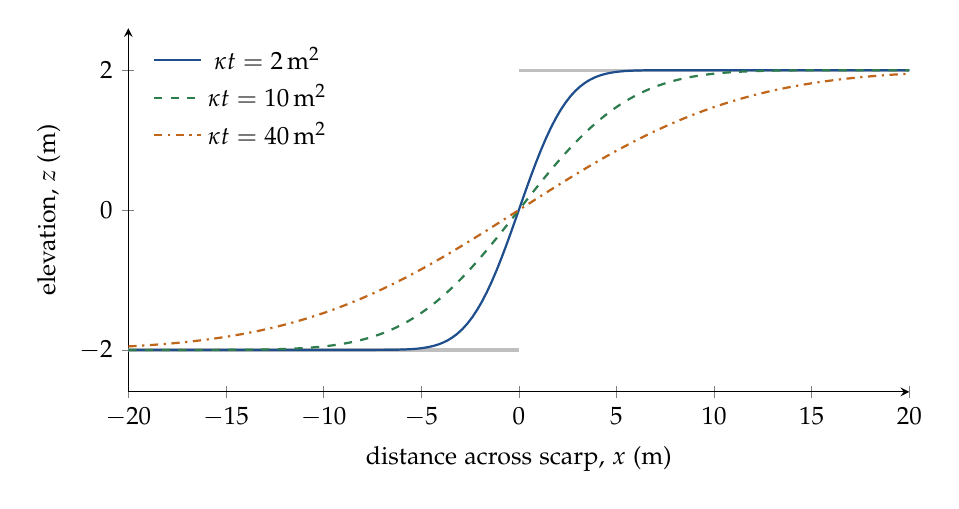
\begin{tikzpicture}
\begin{axis}[width=11.5cm,height=6.2cm,axis lines=left,xlabel={distance across scarp, $x$ (m)},
  ylabel={elevation, $z$ (m)},xmin=-20,xmax=20,ymin=-2.6,ymax=2.6,domain=-20:20,samples=160,
  legend style={draw=none,fill=none,font=\small,at={(0.02,0.98)},anchor=north west},
  tick label style={font=\small},label style={font=\small}]
\addplot[very thick,gray!50,samples=2,domain=-20:0,forget plot] {-2};
\addplot[very thick,gray!50,samples=2,domain=0:20,forget plot] {2};
\addplot[thick,keyblue]              {2*erfa(x/sqrt(4*2))};
\addplot[thick,resgreen,dashed]      {2*erfa(x/sqrt(4*10))};
\addplot[thick,exorange,dash dot]    {2*erfa(x/sqrt(4*40))};
\legend{$\kappa t=2\units{m^2}$,$\kappa t=10\units{m^2}$,$\kappa t=40\units{m^2}$}
\end{axis}
\end{tikzpicture}\par
{\small\itshape A fault scarp relaxing by hillslope diffusion, $z=a\,\erf\!\big(x/\sqrt{4\kappa t}\big)$ --- partial derivatives,\\
a similarity variable and a Gaussian (a smoothed Dirac delta) in one picture (Sections~1, 2 and 4).\par}
\vfill
{\large English edition \quad$\cdot$\quad Version 1.0 \quad$\cdot$\quad September 2026\par}
\vspace{0.4cm}
{\small Source text: P.\,K. Kundu, I.\,M. Cohen \& D.\,R. Dowling, \emph{Fluid Mechanics}, 6th ed.,
Academic Press (2016), Appendix~B ``Mathematical Tools and Resources'', pp.~885--898.\par}
\end{titlepage}

% =====================================================================
%                         HOW TO USE THIS GUIDE
% =====================================================================
\pagenumbering{roman}
\section*{How to use this guide}
\addcontentsline{toc}{section}{How to use this guide}
\markboth{How to use this guide}{}

This guide is a companion to Appendix~B of \citet{kundu2016} (``\Kundu'' below). Each of
Sections~\ref{sec:B1}--\ref{sec:B6} mirrors one section of the appendix (B.1--B.6) and follows the same arc:
\begin{enumerate}[label=\arabic*.,leftmargin=2em]
  \item \textbf{Where it is in your PDF} (page and equation numbers) and \textbf{learning goals};
  \item a \textbf{clear explanation} that rebuilds the intuition behind each formula, with derivations;
  \item \textbf{worked examples} (including \Kundu's Examples B.1--B.4, re-worked in more detail);
  \item a short \textbf{Python check} (SymPy/NumPy/SciPy) that verifies a result, so you can experiment;
  \item a \textbf{research connection} to the dynamics of Earth-surface systems (rivers, hillslopes,
        coasts, sediment transport, groundwater, landscape evolution);
  \item a \textbf{summary} and a set of graded \textbf{exercises}, with full solutions in Appendix~\ref{app:solutions}.
\end{enumerate}
Section~\ref{sec:capstone} is a capstone that combines B.1--B.4 to explain a celebrated
self-organisation mechanism on sandy coastlines. Appendix~\ref{app:formulas} is a two-page formula sheet.

\subsection*{Legend}
\begin{keyidea}[the one thing to take away]The central concept of a subsection.\end{keyidea}\vspace{-4pt}
\begin{pitfall}[a classic mistake]Mistakes that are easy to make and hard to notice.\end{pitfall}\vspace{-4pt}
\begin{research}[Earth-surface dynamics]Where the tool shows up in current research, with references.\end{research}\vspace{-4pt}
\begin{tcolorbox}[guidebox,colback=exorange!3,colframe=exorange!85!black,
  title={Exercise~$n.m$\enspace\lvl{2}\enspace Exercise title\hfill{\normalfont\small solution\,$\blacktriangleright$}}]
Difficulty: \lvl{1} practice and recall;\quad \lvl{2} derivation or application;\quad
\lvl{3} research-level or open-ended. The link in the title bar jumps to the solution.
\end{tcolorbox}

\subsection*{Conventions}
\begin{itemize}
  \item Equation numbers in \textcolor{srcpurple}{purple}, e.g.\ (\textcolor{srcpurple}{B.1.4}),
        are \Kundu's own numbers, so you can find the same equation in your PDF.
        Black numbers such as (1.3) belong to this guide.
  \item Solutions are printed when \verb|\showsolutionstrue| is set near the top of the source file;
        use \verb|\showsolutionsfalse| to produce a problems-only version for self-testing.
  \item All Python snippets run with Python $\geq 3.9$ and NumPy, SciPy and SymPy; the printed
        output is shown in comments (\texttt{\# -> ...}).
\end{itemize}

\subsection*{Notation}
\begin{center}
\small
\begin{tabularx}{\linewidth}{@{}>{\raggedright\arraybackslash}p{0.34\linewidth}X@{}}
\toprule
Symbol & Meaning \\ \midrule
$\xx=(x,y,z)=(x_1,x_2,x_3)$ & position vector (bold upright = vector) \\
$\uu=(u,v,w)=(u_1,u_2,u_3)$ & fluid velocity \\
$(R,\varphi,z)$; \ $\e{R},\e{\varphi},\e{z}$ & cylindrical coordinates and unit vectors (\Kundu's notation) \\
$(r,\theta)$; \ $\e{r},\e{\theta}$ & plane polar coordinates (\Kundu\ B.6) \\
$(r,\theta,\varphi)$; \ $\e{r},\e{\theta},\e{\varphi}$ & spherical coordinates: $\theta$ = polar angle from $+z$ (co-latitude), $\varphi$ = azimuth \\
$\partial/\partial t$, \ $d/dt$, \ $D/Dt$ & partial derivative, total derivative along a path, material derivative \\
$\delta(x)$, \ $\delta_{ij}$, \ $\varepsilon_{ijk}$ & Dirac delta, Kronecker delta, Levi-Civita (alternating) symbol \\
$a_ib_i\equiv\sum_i a_ib_i$ & summation convention on repeated indices \\
$\bomega=\nabla\times\uu$, \ $S_{ij}$ & vorticity, strain-rate tensor \\
$\eta$ & a similarity (combination) variable, as in \Kundu\ B.2 \\
\midrule
$z$, $z_b$, $h$, $\zeta$ & land-surface or bed elevation, flow depth, water-surface elevation \\
$\Up$, $K$, $A$, $S$, $m$, $n$ & rock-uplift rate, erodibility, drainage area, channel slope, stream-power exponents \\
$\qq_s$, $\lambda_p$, $\kappa$ & sediment volume flux per unit width, bed porosity, hillslope diffusivity \\
\bottomrule
\end{tabularx}
\end{center}

\begin{pitfall}[symbol collisions between fluid mechanics and geomorphology]
The two literatures reuse letters: $U$ is a flow speed in fluid mechanics but often a rock-uplift rate
in geomorphology (written $\Up$ here); $A$ is a surface area in Gauss' theorem but a drainage area in
stream-power models; $S$ is a slope, a storativity, or (as $S_{ij}$) a strain rate; $\kappa$ is a
diffusivity but also von K\'arm\'an's constant ($\kappa_{\mathrm{vK}}\approx0.41$ here); and $\delta$ is a
Dirac delta, a Kronecker delta, or a boundary-layer thickness. Always re-read the definitions.
\end{pitfall}

\clearpage
% =====================================================================
%                          DIAGNOSTIC WARM-UP
% =====================================================================
\section*{Warm-up: a ten-minute diagnostic}
\addcontentsline{toc}{section}{Warm-up: a ten-minute diagnostic}
\markboth{Warm-up diagnostic}{}
Try each question in about a minute, without notes. Answers are in Appendix~\ref{app:quiz}.
If you answer eight or more with confidence, skim the corresponding section and go straight
to its research connection and exercises; otherwise study the section carefully.

\begin{quizbox}[Diagnostic questions]
\begin{enumerate}[label=\textbf{Q\arabic*.},leftmargin=2.4em]
  \item (\S\ref{sec:B1}) A thermometer fixed at a river gauge reads a constant temperature all day. Does every water parcel passing the gauge keep a constant temperature?
  \item (\S\ref{sec:B1}) Solve $\partial f/\partial t+3\,\partial f/\partial x=0$ with $f(x,0)=e^{-x^2}$.
  \item (\S\ref{sec:B2}) With $\xi=x-Ut$ and $\tau=t$, express $\partial/\partial t$ (at fixed $x$) and $\partial/\partial x$ (at fixed $t$) in terms of $\partial/\partial\xi$ and $\partial/\partial\tau$.
  \item (\S\ref{sec:B2}) Which combination of $x$ and $t$ turns $\partial c/\partial t=D\,\partial^2 c/\partial x^2$ (infinite domain, step initial condition) into an ODE?
  \item (\S\ref{sec:B3}) What are $\nabla\cdot(\nabla\times\uu)$ and $\nabla\times(\nabla\phi)$?
  \item (\S\ref{sec:B3}) State Gauss' divergence theorem. Why is $\nabla\cdot\qq$ called the ``net outflow per unit volume''?
  \item (\S\ref{sec:B4}) Evaluate $\int_{-\infty}^{\infty}e^{x}\,\delta(x-2)\,dx$ and $\int_{-\infty}^{\infty}\delta(3x)\,dx$. If $x$ is in metres, what are the units of $\delta(x)$?
  \item (\S\ref{sec:B5}) What is the area element on a sphere of radius $a$? Why is $\partial\e{R}/\partial\varphi\neq 0$?
  \item (\S\ref{sec:B6}) Why does the radial Navier--Stokes equation in cylindrical coordinates contain $-u_\varphi^2/R$, although no such term appears in Cartesian coordinates?
  \item (\S\ref{sec:B6}) Is the flow $u_\varphi=\Gamma/(2\pi R)$, $u_R=u_z=0$ rotational?
\end{enumerate}
\end{quizbox}

\clearpage
\tableofcontents
\clearpage
\pagenumbering{arabic}

\clearpage
% =====================================================================
\section{Partial and Total Differentiation}\label{sec:B1}
% =====================================================================
\begin{source}
\textbf{In your PDF:} \Kundu\ \S B.1, pp.~885--889 --- Eqs.~(B.1.1)--(B.1.16), Example~B.1,
and ``Integration of Partial Derivatives''.
\end{source}

\begin{goals}
\begin{itemize}
  \item Distinguish $\partial/\partial t$, $d/dt$ along a path, and $D/Dt$, and convert between them.
  \item Solve first-order PDEs with the method of characteristics, including source terms and boundary data.
  \item Integrate partial derivatives correctly (the ``constant'' of integration is a function).
  \item \emph{Extension:} differentiate integrals with moving limits and use the kinematic boundary condition.
\end{itemize}
\end{goals}

\subsection{Fields, and two ways of watching them}
Almost everything in fluid mechanics is a \emph{field}: a quantity $f(\xx,t)=f(x_1,x_2,x_3,t)$ attached to every
point in space at every instant --- velocity, pressure, temperature, suspended-sediment concentration, or the
elevation of a river bed. There are two natural ways to observe a field:
\begin{itemize}
  \item \textbf{Eulerian} observation at a fixed point: a stream gauge, a moored current meter, a sediment trap, a tide gauge;
  \item \textbf{Lagrangian} observation that moves with the material: a surface drifter, a dye patch, an RFID-tagged pebble, a single sand grain.
\end{itemize}
Both observers see the same field, but they record \emph{different rates of change}. Section B.1 is the
bookkeeping that connects them.

\subsection{Partial derivatives}
The partial derivative $\partial f/\partial t$ differentiates with respect to $t$ while \emph{all other
independent variables are held fixed}:
\begin{equation}
\pd{f}{t}\equiv\left(\pd{f}{t}\right)_{\!\xx}=\lim_{\Delta t\to0}\frac{f(\xx,t+\Delta t)-f(\xx,t)}{\Delta t}.
\end{equation}
The subscript $\xx$ (``at fixed $\xx$'') is usually omitted, but it is worth writing whenever you change
variables (Section~\ref{sec:B2}), because ``fixed $\xx$'' and ``fixed something else'' give different answers.
Mixed partial derivatives commute, $\partial^2 f/\partial t\,\partial x_i=\partial^2 f/\partial x_i\,\partial t$,
provided the second derivatives are continuous (Schwarz's theorem). This holds for smooth flows but fails
across discontinuities such as hydraulic jumps, bores, or the idealised lee face of a dune.

\subsection{The total derivative along a path}
Suppose an observer moves along a prescribed path $\xx=\XX(t)=(X_1(t),X_2(t),X_3(t))$ --- a boat, a drone, or
a fluid parcel. The value she records is $F(t)=f(\XX(t),t)$, and the chain rule gives \citep[p.~886]{kundu2016}
\begin{equation}\label{eq:totalderiv}
\od{F}{t}=\od{}{t}f(\XX(t),t)=\pd{f}{t}+\pd{f}{x_1}\od{X_1}{t}+\pd{f}{x_2}\od{X_2}{t}+\pd{f}{x_3}\od{X_3}{t}.
\end{equation}
There are two contributions: the field changes in time at a fixed point (first term), and the observer
samples a spatially varying field as she moves (remaining terms). Without a path, ``$df/dt$'' has no meaning.

\subsection{The material derivative}
Now choose the path of a fluid particle. Its velocity is the fluid velocity at its own location,
\begin{equation}
\od{\XX}{t}=\uu(\XX(t),t)\qquad\Longleftrightarrow\qquad \od{X_i}{t}=u_i, \ktag{B.1.2--B.1.3}
\end{equation}
and substituting into \eqref{eq:totalderiv} gives the \emph{material} (substantial, Lagrangian) derivative
\begin{equation}\label{eq:matderiv}
\Dt{f}=\pd{f}{t}+u_1\pd{f}{x_1}+u_2\pd{f}{x_2}+u_3\pd{f}{x_3}=\pd{f}{t}+\uu\cdot\nabla f=\pd{f}{t}+u_i\pd{f}{x_i}. \ktag{B.1.4}
\end{equation}

\begin{keyidea}[local change $+$ advective change]
Read \eqref{eq:matderiv} backwards: a fixed probe sees $\partial f/\partial t = Df/Dt-\uu\cdot\nabla f$.
The reading at a fixed point changes either because the parcels themselves change ($Df/Dt\neq0$) or because
the flow brings \emph{different} parcels, carrying different values, to the probe ($-\uu\cdot\nabla f$).
If $Df/Dt=0$, the quantity is \emph{materially conserved}: each parcel keeps its value and all Eulerian change
is due to advection. Newton's second law applies to parcels, which is why the Navier--Stokes equations contain
$D\uu/Dt=\partial\uu/\partial t+(\uu\cdot\nabla)\uu$.
\end{keyidea}

\begin{worked}[Eulerian versus Lagrangian at a river gauge]\label{we:gauge}
At a gauging station the suspended-sediment concentration is falling at
$\partial C/\partial t=-0.020\units{kg\,m^{-3}\,h^{-1}}$. A survey shows that $C$ increases downstream at
$\partial C/\partial x=+0.004\units{kg\,m^{-3}\,km^{-1}}$ (the water now farther downstream passed the upstream reaches
earlier, when the river was more turbid), and the mean velocity is
$u=1.2\units{m\,s^{-1}}$. What is happening to the water parcels themselves?

\emph{Solution.} Convert $u$ to $4.32\units{km\,h^{-1}}$. Then
\[
\Dt{C}=\pd{C}{t}+u\pd{C}{x}=-0.020+4.32\times0.004=-0.020+0.0173=-0.0027\units{kg\,m^{-3}\,h^{-1}}.
\]
Most of the decline seen at the gauge ($0.0173$ of $0.020$) is advective: cleaner water from upstream is
arriving. The parcels themselves lose sediment only slowly (net settling), about seven times more slowly than the
gauge record suggests.
\end{worked}

\begin{pitfall}[$D/Dt$ does not commute with spatial derivatives]
Differentiating \eqref{eq:matderiv} with respect to $x_j$ gives
$\displaystyle \pd{}{x_j}\Dt{f}=\Dt{}\!\left(\pd{f}{x_j}\right)+\pd{u_i}{x_j}\pd{f}{x_i}$.
Even if $Df/Dt=0$, the \emph{gradient} of $f$ is not conserved: velocity gradients stretch and rotate it.
This is why converging flows sharpen fronts (e.g.\ salinity fronts in estuaries).
\end{pitfall}

\subsection{First-order PDEs and the method of characteristics}
Kundu considers the first-order PDE
\begin{equation}\label{eq:B15}
A(x,t)\pd{f}{t}+B(x,t)\pd{f}{x}=g(x,t,f). \ktag{B.1.5}
\end{equation}
The idea is to find curves $C$ in the $x$--$t$ plane along which the left-hand side is an ordinary derivative.
Parametrise $C$ by $s$, i.e.\ $t=T(s)$, $x=X(s)$. By the chain rule,
$df/ds=(\partial f/\partial t)(dT/ds)+(\partial f/\partial x)(dX/ds)$ \textcolor{srcpurple}{(B.1.6)}, which matches
\eqref{eq:B15} if
\begin{equation}\label{eq:charODE}
\od{T}{s}=A,\qquad \od{X}{s}=B,\qquad \od{f}{s}=g, \ktag{B.1.7}
\end{equation}
so that the characteristic curves satisfy $dX/dT=B(X,T)/A(X,T)$ \textcolor{srcpurple}{(B.1.8)}. (Fine print:
\Kundu\ calls $s$ the arc length, but any parameter along $C$ works; with the choice \eqref{eq:charODE}, $s$ is
the arc length only if $A^2+B^2=1$.)

\begin{keyidea}[a recipe for the method of characteristics]
\begin{enumerate}[label=\arabic*.,leftmargin=1.6em]
  \item Write the characteristic ODEs: $dt/ds=A$, $dx/ds=B$, $df/ds=g$.
  \item Attach data: at $s=0$, $t=0$, $x=X_0$ and $f=\phi(X_0)$ (initial data), or $x=0$, $t=T_0$ and
        $f=f_{\mathrm{in}}(T_0)$ (boundary data).
  \item Integrate the three ODEs.
  \item Eliminate $s$ and the label $X_0$ (or $T_0$) to obtain $f(x,t)$.
\end{enumerate}
\Kundu's two lessons (p.~888): PDEs are solved by rearrangement and \emph{integration}, not by further
differentiation; and the difficulty is not removed but moved --- one unknown $f(x,t)$ of two variables becomes two
unknowns $f(s)$ and $X(s)$ of one variable.
\end{keyidea}

\begin{worked}[Example B.1 revisited: a signal carried by a time-varying current]\label{we:B1}
Solve $\partial f/\partial t+U(t)\,\partial f/\partial x=0$ with $f(x,0)=\phi(x)$ \textcolor{srcpurple}{(B.1.9--B.1.10)}.

Here $A=1$, $B=U(t)$, $g=0$. Step 1: $dT/ds=1$, $dX/ds=U(T)$, $df/ds=0$. Step 2--3: $T=s$,
$X=X_0+\int_0^{s}U(\tau)\,d\tau$ and $f=\phi(X_0)$ along each curve. Step 4: eliminate $s=t$ and
$X_0=x-\int_0^tU(\tau)\,d\tau$:
\begin{equation}\label{eq:B116}
f(x,t)=\phi\!\left(x-\int_0^tU(\tau)\,d\tau\right). \ktag{B.1.16}
\end{equation}
The initial profile is translated, undistorted, by the accumulated displacement $\int_0^tU\,d\tau$.
Because $U$ depends on $t$ only, every characteristic is a horizontal translate of every other one
(\cref{fig:characteristics}a), so they never cross. For constant $U$ we recover the travelling wave
$f=\phi(x-Ut)$.
\end{worked}

\begin{worked}[a source term: decay or settling during transport]\label{we:decay}
Solve $\partial f/\partial t+U\,\partial f/\partial x=-\lambda f$, $f(x,0)=\phi(x)$, with constant $U$ and $\lambda$.

With $A=1$, $B=U$, $g=-\lambda f$: $T=s$, $X=X_0+Us$, and $df/ds=-\lambda f$, so $f=\phi(X_0)\,e^{-\lambda s}$.
Eliminating $s=t$, $X_0=x-Ut$:
\[
f(x,t)=\phi(x-Ut)\,e^{-\lambda t}.
\]
The pattern is advected \emph{and} decays along each characteristic. With $\lambda=w_s/h$ this describes fine
sediment settling out of a well-mixed flow of depth $h$ (Exercise~\ref{ex:settling}); with $\lambda$ a decay
constant it describes a radioactive or reactive tracer.
\end{worked}

\paragraph{When the speed depends on the solution: breaking and shocks.}
If the propagation speed depends on $f$ itself, $\partial f/\partial t+c(f)\,\partial f/\partial x=0$, then $f$ is
still constant along characteristics, which are therefore \emph{straight} lines $x=X_0+c(\phi(X_0))\,t$ --- but
with slopes that depend on the initial value. Where larger values of $c$ start behind smaller ones, the lines
converge and first cross at the breaking time $t_b=1/\max_{X_0}\!\big[-\,d c(\phi(X_0))/dX_0\big]$
(\cref{fig:characteristics}b). Beyond $t_b$ the formal solution is multivalued, and a discontinuity (a
\emph{shock}) forms. For a conservation law $\partial f/\partial t+\partial q(f)/\partial x=0$ it moves at the
speed $V=[q]/[f]=(q_2-q_1)/(f_2-f_1)$ fixed by mass conservation across the jump.

\begin{figure}[htbp]
\centering
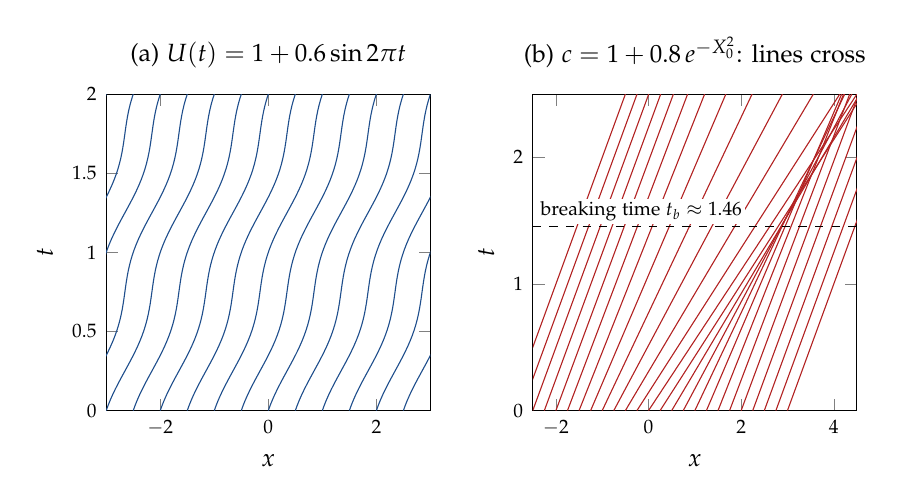
\begin{tikzpicture}
\begin{axis}[name=A,width=0.47\linewidth,height=5.6cm,xmin=-3,xmax=3,ymin=0,ymax=2,
  xlabel={$x$},ylabel={$t$},title={\small (a) $U(t)=1+0.6\sin 2\pi t$},
  tick label style={font=\scriptsize},label style={font=\small}]
\pgfplotsinvokeforeach{-5,-4.5,...,2.5}{
  \addplot[keyblue,thin,domain=0:2,samples=60,variable=\t] ({#1+\t+0.0955*(1-cos(360*\t))},{\t});}
\end{axis}
\begin{axis}[at={(A.east)},anchor=west,xshift=1.3cm,width=0.47\linewidth,height=5.6cm,
  xmin=-2.5,xmax=4.5,ymin=0,ymax=2.5,xlabel={$x$},ylabel={$t$},
  title={\small (b) $c=1+0.8\,e^{-X_0^2}$: lines cross},
  tick label style={font=\scriptsize},label style={font=\small}]
\pgfplotsinvokeforeach{-3,-2.75,...,3}{
  \addplot[pitred,thin,domain=0:2.5,samples=2,variable=\t] ({#1+(1+0.8*exp(-(#1)^2))*\t},{\t});}
\addplot[black,dashed,domain=-2.5:4.5,samples=2] {1.457};
\node[font=\scriptsize,anchor=south west,fill=white,inner sep=1pt] at (axis cs:-2.4,1.47) {breaking time $t_b\approx1.46$};
\end{axis}
\end{tikzpicture}
\caption{Characteristics in the $x$--$t$ plane. (a) Example B.1 with a time-dependent speed: all curves are
translates of one another and never cross. (b) A nonlinear kinematic wave whose speed depends on the transported
quantity: faster characteristics overtake slower ones and a shock forms at $t_b$.}
\label{fig:characteristics}
\end{figure}

\subsection{Integrating partial derivatives}
Integrating a partial derivative is ordinary integration with the other variables frozen, so the ``constant''
of integration may depend on all of them \citep[pp.~888--889]{kundu2016}:
\begin{equation}
\pd{f}{x}=Ax+By\quad\Longrightarrow\quad f=\int(Ax+By)\,dx=\tfrac12Ax^2+Byx+C(y,z,t).
\end{equation}
If \emph{both} $\partial f/\partial x=P(x,y)$ and $\partial f/\partial y=Q(x,y)$ are prescribed, a solution exists only
if the mixed partials agree, $\partial P/\partial y=\partial Q/\partial x$. This compatibility condition is the
two-dimensional version of ``a curl-free field is a gradient'' (Section~\ref{sec:B3}, identity (B.3.11)); see
Exercise~\ref{ex:integrate}.

\subsection{Toolbox extension: integrals with moving limits and the kinematic boundary condition}
Two results that are not in \Kundu's appendix are used constantly in depth-averaged Earth-surface models.
\textbf{Leibniz' rule} differentiates an integral whose limits move:
\begin{equation}\label{eq:leibniz}
\od{}{x}\int_{a(x)}^{b(x)}f(x,z)\,dz=\int_{a}^{b}\pd{f}{x}\,dz+f(x,b)\,\od{b}{x}-f(x,a)\,\od{a}{x}.
\end{equation}
The \textbf{kinematic boundary condition} states that a surface $F(\xx,t)=0$ that moves with the fluid (no fluid
crosses it) is materially conserved, $DF/Dt=0$ on $F=0$. For a free surface $z=\zeta(x,y,t)$, take
$F=z-\zeta$:
\begin{equation}\label{eq:kbc}
w=\pd{\zeta}{t}+u\pd{\zeta}{x}+v\pd{\zeta}{y}\qquad\text{at } z=\zeta(x,y,t).
\end{equation}
Integrating the continuity equation over the depth with \eqref{eq:leibniz} and \eqref{eq:kbc} gives
$\partial h/\partial t+\nabla_h\cdot(h\bar{\uu})=0$ (Exercise~\ref{ex:leibniz}), the backbone of the shallow-water
(Saint-Venant) equations used for floods, sheet flow, turbidity currents and river morphodynamics.

\subsection{Research connection: kinematic waves on Earth's surface}
\begin{research}[conservation law $+$ flux law $=$ kinematic wave]
A large part of Earth-surface dynamics has the structure
\begin{equation}\label{eq:kinwave}
\pd{a}{t}+\pd{q}{x}=s,\qquad q=q(a,x)\quad\Longrightarrow\quad
\pd{a}{t}+c\,\pd{a}{x}=s-\left.\pd{q}{x}\right|_{a},\qquad c=\pd{q}{a},
\end{equation}
where $a$ is a stored quantity and $q$ its flux. By \eqref{eq:charODE}, disturbances in $a$ travel along
characteristics at the \emph{kinematic-wave speed} $c=\partial q/\partial a$, which is generally \emph{not} the
speed of the material itself.
\begin{itemize}[leftmargin=1.2em]
  \item \textbf{Flood waves} \citep{lighthill1955}. With cross-section $a=A$ and discharge $Q(A)$, $c=dQ/dA$.
        In a wide channel with Ch\'ezy friction, $U\propto h^{1/2}$ and $c=\tfrac32U$; with Manning friction,
        $c=\tfrac53U$. Flood peaks outrun the water, and because $c$ grows with depth, rising limbs steepen into
        kinematic shocks (Exercise~\ref{ex:flood}).
  \item \textbf{Knickpoints in bedrock rivers.} The stream-power incision model is
        $\partial z/\partial t=\Up-KA^mS^n$, with $x$ measured upstream from base level and $S=\partial z/\partial x$.
        For $n=1$ it is exactly \eqref{eq:B15}:
        \begin{equation}\label{eq:streampower}
        \pd{z}{t}+K A(x)^m\pd{z}{x}=\Up .
        \end{equation}
        Knickpoints are characteristics travelling \emph{upstream} at $c=KA^m$, slowing as drainage area
        decreases \citep{rosenbloom1994,whipple1999}. The time for a signal to reach $x$ is
        $\tau(x)=\int_0^x dx'/(KA(x')^m)$, a basic landscape response time (Exercise~\ref{ex:knick}).
        For $n\neq1$ (and spatially uniform $\Up$) the slope obeys $\partial S/\partial t+\partial(KA^mS^n)/\partial x=0$, a nonlinear kinematic
        wave with $c=nKA^mS^{n-1}$, so knickpoints can sharpen or spread out.
  \item \textbf{Bedforms.} The Exner equation $(1-\lambda_p)\,\partial z_b/\partial t+\partial q_s/\partial x=0$
        and a bedload flux that increases with bed elevation faster than linearly (e.g.\ Exner's classical
        $q_s\propto\bar u\propto1/(\zeta-z_b)$, with $\zeta$ the water surface) gives
        $c=(1-\lambda_p)^{-1}\partial q_s/\partial z_b>0$ with $\partial c/\partial z_b>0$. Crests move faster than troughs, so lee faces steepen
        into avalanche faces --- shocks in the sense of \cref{fig:characteristics}b. Section~\ref{sec:B2} turns
        this around to measure bedload by ``dune tracking''.
  \item \textbf{Lagrangian archives.} Tracer pebbles, dye, drifters and in-situ cosmogenic nuclides record
        Lagrangian histories; converting them to Eulerian rates is an application of \eqref{eq:matderiv}
        (Exercise~\ref{ex:cosmo}).
\end{itemize}
\end{research}

\begin{pycode}[Example B.1 symbolically, and knickpoint travel times numerically]
import sympy as sp
x, t, tau = sp.symbols('x t tau', real=True)
U0, U1, w = sp.symbols('U_0 U_1 omega', positive=True)
phi = sp.Function('phi')                  # arbitrary initial profile
U = lambda s: U0 + U1*sp.sin(w*s)         # a time-dependent speed U(t)
f = phi(x - sp.integrate(U(tau), (tau, 0, t)))       # candidate (B.1.16)
print(sp.simplify(sp.diff(f, t) + U(t)*sp.diff(f, x)))   # -> 0
print(f.subs(t, 0))                       # -> phi(x): initial condition

import numpy as np
from scipy.integrate import solve_ivp
K, ka, m, L = 2e-6, 1.0, 0.5, 20e3   # K [1/yr]; A = ka*(L-x)^2 [m^2]; L [m]
def celerity(t, x):                  # dx/dt = K A(x)^m, x upstream
    return K*(ka*(L - x)**2)**m
def near_divide(t, x):               # stop 1 km from the divide
    return x[0] - (L - 1e3)
near_divide.terminal = True
sol = solve_ivp(celerity, [0, 1e8], [0.0], events=near_divide,
                rtol=1e-10, atol=1e-8)
t_num = sol.t_events[0][0]/1e6
t_exact = np.log(L/1e3)/(K*np.sqrt(ka))/1e6
print(f"{t_num:.4f} Myr (numerical), {t_exact:.4f} Myr (exact)")
# -> 1.4979 Myr (numerical), 1.4979 Myr (exact)
\end{pycode}

\begin{remember}
\begin{itemize}
  \item $d/dt$ needs a path; $D/Dt=\partial/\partial t+\uu\cdot\nabla$ is $d/dt$ along a fluid-particle path.
  \item A fixed probe sees parcel change \emph{plus} advection of different parcels past it.
  \item First-order PDEs become ODEs along characteristics; information propagates along them, and crossing
        characteristics signal shocks.
  \item Partial integration produces functions, not constants, of the remaining variables.
  \item Flood waves, knickpoints and bedforms are kinematic waves with speed $c=\partial q/\partial a$.
\end{itemize}
\end{remember}

\subsection*{Exercises for Section~\ref{sec:B1}}

\begin{exercise}[Three derivatives of one field]{1}{threederiv}
Let $f(x,y,t)=x^2y\,e^{-t}$.
(a) Compute $\partial f/\partial t$, $\partial f/\partial x$, and verify that $\partial^2f/\partial x\,\partial t=\partial^2 f/\partial t\,\partial x$.
(b) Compute $df/dt$ along the path $X(t)=t$, $Y(t)=1+t^2$, first with \eqref{eq:totalderiv} and then by
substituting the path into $f$ before differentiating.
(c) Compute $Df/Dt$ in the two-dimensional flow $u=-y$, $v=x$ (solid-body rotation).
\end{exercise}

\begin{exercise}[A patch stretched by a diverging flow]{1}{stretch}
Solve $\partial f/\partial t+a\,x\,\partial f/\partial x=0$ with $f(x,0)=\phi(x)$ and constant $a>0$, i.e.\ a scalar
carried by the diverging flow $u=ax$. For $\phi(x)=\exp(-x^2/\ell^2)$, how does the width of the patch change in
time? What changes if $a<0$?
\end{exercise}

\begin{exercise}[How far does fine sediment travel?]{2}{settling}
Well-mixed fine sediment enters a reach of steady, uniform flow (depth $h$, speed $U$) at $x=0$ with
concentration $C_{\mathrm{in}}$ from $t=0$ onward; the reach is initially clear, $C(x,0)=0$ for $x>0$. Settling removes
sediment at the rate $w_sC/h$, so that $\partial C/\partial t+U\,\partial C/\partial x=-(w_s/h)\,C$.
(a) Sketch the characteristics and find $C(x,t)$ in the regions $x>Ut$ and $x<Ut$.
(b) Show that behind the front the profile is steady and decays over an ``advection length''
$L_s=Uh/w_s$. Evaluate $L_s$ for $U=1\units{m\,s^{-1}}$, $h=2\units{m}$ and $w_s=1\units{mm\,s^{-1}}$
(coarse silt, $d\approx30\units{\mu m}$; cf.\ Section~\ref{sec:B6}).
\end{exercise}

\begin{exercise}[Knickpoints slow down as they climb]{2}{knick}
In \eqref{eq:streampower} take $m=1/2$ and a Hack-like drainage-area distribution $A(x)=k_a(L-x)^2$, where $x$ is
distance upstream from the outlet and $L$ is the distance from outlet to divide.
(a) Show that a knickpoint released at the outlet at $t=0$ is at $L-x_k(t)=L\,e^{-\beta t}$, with $\beta=K\sqrt{k_a}$.
(b) How long does it take to arrive $1\units{km}$ from the divide if $L=20\units{km}$ and $\beta=2\times10^{-6}\units{yr^{-1}}$?
Compare with the Python check above.
(c) Does the knickpoint ever reach the divide? What physics missing from \eqref{eq:streampower} takes over near
channel heads?
\end{exercise}

\begin{exercise}[Kinematic flood waves]{2}{flood}
For a wide rectangular channel the discharge per unit width is $q=Uh$.
(a) Show that the kinematic-wave speed is $c=dq/dh=\tfrac32U$ for Ch\'ezy friction ($U=C_z\sqrt{hS_0}$) and
$c=\tfrac53U$ for Manning friction ($U=n_M^{-1}h^{2/3}S_0^{1/2}$).
(b) Evaluate $c$ for $U=2\units{m\,s^{-1}}$.
(c) Explain, using characteristics, why the rising limb of a flood wave steepens.
(d) A kinematic shock separates depths $h_1$ (ahead) and $h_2>h_1$ (behind). Write its speed for Ch\'ezy friction.
\end{exercise}

\begin{exercise}[Integrating partial derivatives]{1}{integrate}
(a) Find the general solution of $\partial^2 f/\partial x\,\partial y=0$.
(b) Find $f(x,y)$ such that $\partial f/\partial x=2xy+1$ and $\partial f/\partial y=x^2+\cos y$.
(c) Show that no $f$ satisfies $\partial f/\partial x=-y$ and $\partial f/\partial y=x$. Which velocity field is
$(-y,x)$, and what does this say about writing it as the gradient of a potential?
\end{exercise}

\begin{exercise}[Depth-averaged continuity from Leibniz' rule]{2}{leibniz}
Consider two-dimensional flow $(u,w)$ over a fixed, impermeable bed $z=z_b(x)$, with free surface $z=\zeta(x,t)$ and
depth $h=\zeta-z_b$. Integrate $\partial u/\partial x+\partial w/\partial z=0$ from $z_b$ to $\zeta$. Use
\eqref{eq:leibniz}, the kinematic condition \eqref{eq:kbc} at the surface, and $w=u\,dz_b/dx$ at the bed to show that
\[
\pd{h}{t}+\pd{(h\bar u)}{x}=0,\qquad \bar u=\frac1h\int_{z_b}^{\zeta}u\,dz .
\]
\end{exercise}

\begin{exercise}[Cosmogenic nuclides: a Lagrangian clock in an eroding hillslope]{3}{cosmo}
In-situ cosmogenic nuclides (e.g.\ $^{10}$Be in quartz) are produced at a rate that decays with depth $Z$ below
the ground surface, $P(Z)=P_0e^{-Z/z_*}$, and decay radioactively at rate $\lambda N$. The surface erodes at a
steady rate $\varepsilon$, so a rock parcel approaches the surface: $dZ/dt=-\varepsilon$.
(a) Write $dN/dt$ following a parcel. Then write the equation for $N(Z,t)$ in a frame attached to the eroding
surface, identifying the ``material derivative'' $\partial/\partial t-\varepsilon\,\partial/\partial Z$.
(b) Find the steady profile $N(Z)$ and show that the surface concentration is $N_0=P_0/(\lambda+\varepsilon/z_*)$
\citep{lal1991}.
(c) Solve for $\varepsilon$ and evaluate it for $N_0=1.0\times10^5\units{atoms\,g^{-1}}$,
$P_0=4\units{atoms\,g^{-1}\,yr^{-1}}$, $z_*=\Lambda/\rho=(160\units{g\,cm^{-2}})/(2.65\units{g\,cm^{-3}})$ and a
half-life of $1.387\units{Myr}$. (Site-specific production scaling is ignored.)
\end{exercise}

\clearpage
% =====================================================================
\section{Changing Independent Variables}\label{sec:B2}
% =====================================================================
\begin{source}
\textbf{In your PDF:} \Kundu\ \S B.2, pp.~889--890 --- Eqs.~(B.2.1)--(B.2.3), Examples~B.2 (moving frames) and
B.3 (similarity variable).
\end{source}

\begin{goals}
\begin{itemize}
  \item Transform derivatives under a change of coordinates with the chain rule (B.2.1).
  \item Always know \emph{what is held constant} when a partial derivative is taken.
  \item Use moving frames to turn migrating patterns into steady ones.
  \item Find similarity variables (B.2.3), choose their exponents, and reduce PDEs to ODEs.
\end{itemize}
\end{goals}

\subsection{The chain rule for new coordinates}
Suppose the new independent variables are $\xi=X(x,y,z,t)$, $\psi=Y(x,y,z,t)$, $\zeta=Z(x,y,z,t)$ and
$\tau=T(x,y,z,t)$ (\Kundu's letters; here $\zeta$ is just a coordinate). A field can be written in either set,
$f(x,y,z,t)=F(\xi,\psi,\zeta,\tau)$, and the chain rule gives, for example,
\begin{equation}\label{eq:B21}
\pd{}{x}=\pd{X}{x}\pd{}{\xi}+\pd{Y}{x}\pd{}{\psi}+\pd{Z}{x}\pd{}{\zeta}+\pd{T}{x}\pd{}{\tau},\qquad
\pd{}{t}=\pd{X}{t}\pd{}{\xi}+\pd{Y}{t}\pd{}{\psi}+\pd{Z}{t}\pd{}{\zeta}+\pd{T}{t}\pd{}{\tau}, \ktag{B.2.1}
\end{equation}
and similarly for $\partial/\partial y$ and $\partial/\partial z$. In matrix form the old derivatives are the
transpose of the Jacobian $\partial(\xi,\psi,\zeta,\tau)/\partial(x,y,z,t)$ acting on the new ones. The recipe
needs the derivatives of the \emph{new variables with respect to the old ones}; if the transformation is given
the other way round, invert the Jacobian or differentiate implicitly.

\begin{worked}[from Cartesian to plane polar derivatives]\label{we:polar}
With $r=\sqrt{x^2+y^2}$ and $\theta=\operatorname{atan2}(y,x)$ we have $\partial r/\partial x=x/r=\cos\theta$,
$\partial r/\partial y=\sin\theta$, $\partial\theta/\partial x=-y/r^2=-\sin\theta/r$ and
$\partial\theta/\partial y=\cos\theta/r$. By \eqref{eq:B21},
\begin{equation}\label{eq:polarderiv}
\pd{}{x}=\cos\theta\,\pd{}{r}-\frac{\sin\theta}{r}\pd{}{\theta},\qquad
\pd{}{y}=\sin\theta\,\pd{}{r}+\frac{\cos\theta}{r}\pd{}{\theta}.
\end{equation}
Applying these twice gives the polar Laplacian of \Kundu\ \S B.6 (Exercise~\ref{ex:polarlap}). This is the
``brute-force'' route; Section~\ref{sec:B5} gives a faster one using scale factors.
\end{worked}

\begin{pitfall}[what is held constant?]
Take $f(x,t)=\sin(x-Ut)$ and the moving coordinate $\xi=x-Ut$, $\tau=t$, so $F(\xi,\tau)=\sin\xi$. Then
$(\partial f/\partial t)_x=-U\cos(x-Ut)$ but $(\partial F/\partial\tau)_\xi=0$. Both are ``the time derivative'',
yet they answer different questions: how fast the signal changes at a fixed place, and how fast it changes for an
observer riding with the pattern. After any change of variables, write the subscripts.
\end{pitfall}

\subsection{Moving frames: Example B.2 revisited}
For frames translating at constant velocity $(U,V,W)$, $\xi=x-Ut$, $\psi=y-Vt$, $\zeta=z-Wt$, $\tau=t$, and
\eqref{eq:B21} gives
\begin{equation}\label{eq:B22}
\pd{}{x}=\pd{}{\xi},\quad\pd{}{y}=\pd{}{\psi},\quad\pd{}{z}=\pd{}{\zeta},\quad
\pd{}{t}=\pd{}{\tau}-U\pd{}{\xi}-V\pd{}{\psi}-W\pd{}{\zeta}. \ktag{B.2.2}
\end{equation}
As \Kundu\ remarks, the simplest-looking transformation, $\tau=t$, produces the most complicated derivative.
The reason is the pitfall above: $\partial/\partial t$ is taken at fixed $x$, whereas $\partial/\partial\tau$ is taken
at fixed $\xi$, i.e.\ following an observer who moves with velocity $(U,V,W)$. Rearranged,
$\partial/\partial\tau=\partial/\partial t+U\partial/\partial x+V\partial/\partial y+W\partial/\partial z$ is precisely the
total derivative \eqref{eq:totalderiv} along a straight path; if the observer moved with the local fluid velocity it
would be $D/Dt$.

Two consequences are used constantly:
\begin{itemize}
  \item \textbf{Galilean invariance.} The advection--diffusion equation
        $\partial f/\partial t+U\partial f/\partial x=\kappa\,\partial^2f/\partial x^2$ becomes pure diffusion,
        $\partial F/\partial\tau=\kappa\,\partial^2F/\partial\xi^2$, in a frame moving with the flow (Exercise~\ref{ex:galilean}).
  \item \textbf{Travelling (``frozen'') patterns.} A pattern that is steady in a frame moving at speed $c$ has
        $f(x,t)=F(x-ct)$ and therefore
        \begin{equation}\label{eq:frozen}
        \pd{f}{t}=-c\,\pd{f}{x}.
        \end{equation}
        This is Taylor's frozen-turbulence hypothesis (which converts a time series from a fixed probe into a spatial
        signal) and the basis of dune tracking, below.
\end{itemize}

\subsection{Similarity variables: Example B.3 revisited}
The second use of a change of variables is to \emph{combine} independent variables and so reduce their number.
If $\eta=H(x,y,z,t)$ and $f$ depends on $\eta$ alone, the chain rule gives \textcolor{srcpurple}{(B.2.3)}
\begin{equation}
\pd{}{x}=\pd{H}{x}\od{}{\eta},\qquad \pd{}{y}=\pd{H}{y}\od{}{\eta},\qquad\pd{}{z}=\pd{H}{z}\od{}{\eta},\qquad
\pd{}{t}=\pd{H}{t}\od{}{\eta}.
\end{equation}
For Kundu's trial variable $\eta=xt^{\alpha}$ (Example B.3),
\begin{equation}\label{eq:B3ex}
\pd{f}{x}=t^{\alpha}\od{f}{\eta},\qquad \pd{f}{t}=\alpha xt^{\alpha-1}\od{f}{\eta}=\frac{\alpha}{t}\,\eta\,\od{f}{\eta},\qquad
\pdd{f}{x}=t^{2\alpha}\frac{d^2f}{d\eta^2}.
\end{equation}

\begin{keyidea}[a recipe for similarity solutions]
\begin{enumerate}[label=\arabic*.,leftmargin=1.6em]
  \item Check that the problem has no intrinsic length or time scale (infinite domain, step or point initial data,
        power-law forcing). Then $x$ and $t$ can only appear in a dimensionless combination.
  \item Postulate $f=t^{\beta}F(\eta)$ with $\eta=xt^{\alpha}$ ($\beta=0$ when the prescribed values are constants).
  \item Substitute, and choose $\alpha$ (and $\beta$) so that $t$ cancels \emph{and} the initial and boundary
        conditions collapse onto conditions on $F(\eta)$.
  \item Solve the resulting ODE.
\end{enumerate}
\end{keyidea}

\begin{worked}[the diffusion equation with a step: the erf solution]\label{we:erf}
Solve $\partial f/\partial t=\kappa\,\partial^2 f/\partial x^2$ on $-\infty<x<\infty$ with $f(x,0)=a\sgn(x)$.

With $\eta=xt^{\alpha}$, \eqref{eq:B3ex} turns the PDE into $(\alpha/t)\,\eta F'=\kappa\,t^{2\alpha}F''$; time cancels only
if $2\alpha=-1$. It is convenient to scale the variable as $\eta=x/\sqrt{4\kappa t}$. Then
$\partial\eta/\partial t=-\eta/(2t)$ and $\partial\eta/\partial x=1/\sqrt{4\kappa t}$, so
\[
-\frac{\eta}{2t}F'=\frac{\kappa}{4\kappa t}F''\quad\Longrightarrow\quad F''+2\eta F'=0
\quad\Longrightarrow\quad F'=C_1e^{-\eta^2}\quad\Longrightarrow\quad F=C_1'\erf(\eta)+C_2,
\]
with $\erf(\eta)=(2/\sqrt\pi)\int_0^{\eta}e^{-s^2}ds$. As $t\to0^+$, $\eta\to\pm\infty$ for $x\gtrless0$, and as
$x\to\pm\infty$ at fixed $t$, $\eta\to\pm\infty$ as well: the initial condition and both boundary conditions collapse onto
$F(\pm\infty)=\pm a$. Hence $C_2=0$, $C_1'=a$ and
\begin{equation}\label{eq:erfsol}
f(x,t)=a\,\erf\!\left(\frac{x}{\sqrt{4\kappa t}}\right).
\end{equation}
Profiles at different times are stretched copies of one curve (\cref{fig:collapse}); the stretching length
$\sqrt{4\kappa t}$ is the diffusion length.
\end{worked}

\begin{figure}[htbp]
\centering
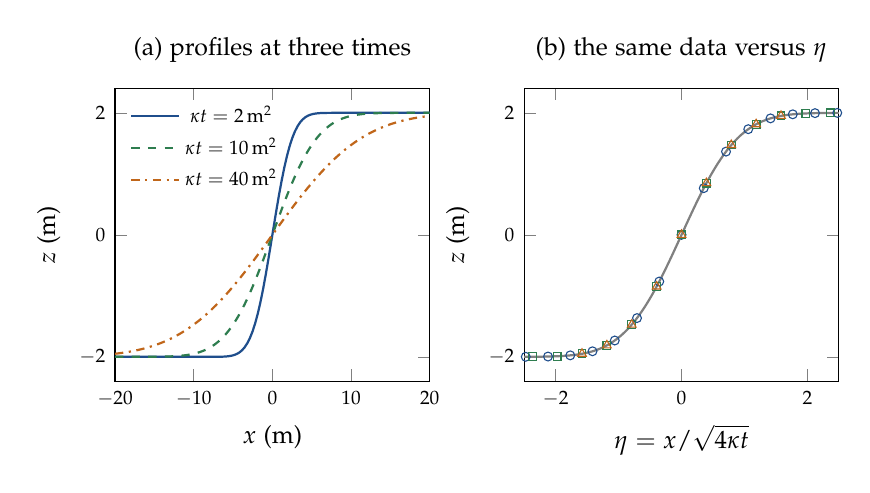
\begin{tikzpicture}
\begin{axis}[name=A,width=0.46\linewidth,height=5.3cm,xmin=-20,xmax=20,ymin=-2.4,ymax=2.4,
  xlabel={$x$ (m)},ylabel={$z$ (m)},title={\small (a) profiles at three times},domain=-20:20,samples=120,
  legend style={font=\scriptsize,draw=none,fill=none,at={(0.02,0.98)},anchor=north west},
  tick label style={font=\scriptsize},label style={font=\small}]
\addplot[thick,keyblue]           {2*erfa(x/sqrt(4*2))};
\addplot[thick,resgreen,dashed]   {2*erfa(x/sqrt(4*10))};
\addplot[thick,exorange,dash dot] {2*erfa(x/sqrt(4*40))};
\legend{$\kappa t=2\units{m^2}$,$\kappa t=10\units{m^2}$,$\kappa t=40\units{m^2}$}
\end{axis}
\begin{axis}[at={(A.east)},anchor=west,xshift=1.2cm,width=0.46\linewidth,height=5.3cm,xmin=-2.5,xmax=2.5,
  ymin=-2.4,ymax=2.4,xlabel={$\eta=x/\sqrt{4\kappa t}$},ylabel={$z$ (m)},title={\small (b) the same data versus $\eta$},
  tick label style={font=\scriptsize},label style={font=\small}]
\addplot[thick,gray,domain=-2.5:2.5,samples=100] {2*erfa(x)};
\addplot[only marks,mark=o,mark size=1.6pt,keyblue,domain=-7:7,samples=15]
  ({x/sqrt(4*2)},{2*erfa(x/sqrt(4*2))});
\addplot[only marks,mark=square,mark size=1.4pt,resgreen,domain=-15:15,samples=13]
  ({x/sqrt(4*10)},{2*erfa(x/sqrt(4*10))});
\addplot[only marks,mark=triangle,mark size=1.8pt,exorange,domain=-20:20,samples=9]
  ({x/sqrt(4*40)},{2*erfa(x/sqrt(4*40))});
\end{axis}
\end{tikzpicture}
\caption{Similarity collapse for the diffusing step \eqref{eq:erfsol} with $a=2\units{m}$ (a degrading fault scarp).
(a) Profiles widen as $\sqrt{\kappa t}$. (b) Plotted against the similarity variable, all times fall on one curve.}
\label{fig:collapse}
\end{figure}

\subsection{Research connection: scarps, river profiles and migrating dunes}
\begin{research}[morphologic dating of scarps]
Hillslope soil transport is often modelled as diffusive, $q_s=-\kappa\,\partial z/\partial x$, so that
$\partial z/\partial t=\kappa\,\partial^2 z/\partial x^2$ \citep{culling1960}. A fresh fault scarp or wave-cut shoreline of
height $2a$ on a regional slope $b$ then degrades as \citep{nash1980,hanks1984}
\begin{equation}\label{eq:scarp}
z(x,t)=a\,\erf\!\left(\frac{x}{\sqrt{4\kappa t}}\right)+b\,x ,
\end{equation}
since $bx$ is a steady solution and the equation is linear. The steepest slope, at $x=0$, is
$S_{\max}=a/\sqrt{\pi\kappa t}+b$, so a measured profile yields the \emph{morphologic age}
$\kappa t=a^2/[\pi(S_{\max}-b)^2]$. Calibrated diffusivities of order $1\units{m^2\,kyr^{-1}}$ in semi-arid settings turn
this into ages. Note that the slope of \eqref{eq:scarp} is a Gaussian: the initial step has slope $2a\,\delta(x)$, and
the slope field diffuses exactly as a Dirac delta does (Section~\ref{sec:B4}). Real applications must handle a
finite initial slope and nonlinear transport on steep slopes \citep{roering1999}.
\end{research}

\begin{research}[the $\chi$ transformation of river profiles]
The knickpoint equation \eqref{eq:streampower} has a variable coefficient $KA(x)^m$. \citet{perron2013} removed it with
a change of independent variable,
\begin{equation}\label{eq:chi}
\chi(x)=\int_0^{x}\left(\frac{A_0}{A(x')}\right)^{m/n}dx'\quad\overset{n=1}{\Longrightarrow}\quad
\pd{z}{t}+KA_0^{m}\pd{z}{\chi}=\Up ,
\end{equation}
with $A_0$ an arbitrary reference area (Exercise~\ref{ex:chi}). In $\chi$-space every knickpoint moves at the same
constant speed $KA_0^m$, so knickpoints released together at base level sit at the same $\chi$ on every tributary. For any $n$,
the steady state is $z=z_{\mathrm{base}}+(\Up/KA_0^m)^{1/n}\chi$: river profiles plot as straight lines in ``$\chi$-plots'', and
departures from linearity reveal transient signals, spatial variations of $\Up/K$, or drainage-divide migration
\citep{willett2014}.
\end{research}

\begin{research}[dune tracking: bedload from a migrating pattern]
If a train of bedforms migrates without changing shape, $z_b(x,t)=F(x-ct)$, then by \eqref{eq:frozen} the Exner
equation $(1-\lambda_p)\,\partial z_b/\partial t+\partial q_s/\partial x=0$ becomes
$\partial q_s/\partial x=(1-\lambda_p)\,c\,\partial z_b/\partial x$, i.e.
\begin{equation}\label{eq:dunetrack}
q_s(x)=(1-\lambda_p)\,c\,z_b(x)+q_0 .
\end{equation}
Measuring $z_b$ relative to the troughs (where $q_s\approx q_0\approx0$ if no sediment bypasses the dunes) and averaging over
one wavelength gives $\bar q_s\approx\beta(1-\lambda_p)\,cH$, with $\beta\approx\tfrac12$ for triangular dunes of height $H$
\citep{simons1965}. Repeated multibeam surveys of large sand-bedded rivers use exactly this Galilean argument.
\end{research}

\paragraph{More similarity solutions in Earth-surface science.} Delta shorelines prograde as $\sqrt t$ in diffusive
basin-filling models, a moving-boundary (Stefan) problem \citep{swenson2000}; viscous gravity currents of lava or mud spread
as $t^{1/5}$ \citep{huppert1982} (Exercise~\ref{ex:gravcurrent}); groundwater drawdown near a pumped well depends on
$r^2/(4Dt)$ (Section~\ref{sec:B6}); and a boundary layer over a suddenly started bed grows as $\sqrt{\nu t}$.

\begin{pycode}[the scarp solution and its morphologic age]
import sympy as sp
x, t, kap, a, b, s = sp.symbols('x t kappa a b S_max', positive=True)
z = a*sp.erf(x/sp.sqrt(4*kap*t)) + b*x          # degraded fault scarp
print(sp.simplify(sp.diff(z, t) - kap*sp.diff(z, x, 2)))   # -> 0
smax = sp.simplify(sp.diff(z, x).subs(x, 0))    # steepest slope, at x = 0
print(smax)            # -> a/(sqrt(pi)*sqrt(kappa)*sqrt(t)) + b
kt = sp.solve(sp.Eq(smax, s), t)[0]*kap         # morphologic age kappa*t
print(sp.simplify(kt), kt.subs({a: 2, b: 0.05, s: 0.30}).evalf(4))
# -> a**2/(pi*(S_max - b)**2) 20.37      (m^2)
\end{pycode}

\begin{remember}
\begin{itemize}
  \item $\partial/\partial(\text{old})=\sum(\partial\,\text{new}/\partial\,\text{old})\,\partial/\partial(\text{new})$; you need the
        derivatives of the new variables with respect to the old ones.
  \item Moving frame: $(\partial/\partial t)_x=(\partial/\partial\tau)_\xi-U\,\partial/\partial\xi$; frozen patterns obey
        $\partial f/\partial t=-c\,\partial f/\partial x$.
  \item Similarity: no intrinsic scales $\Rightarrow$ combine variables; $t$ must cancel and the conditions must collapse.
  \item Diffusion always produces the length $\sqrt{4\kappa t}$; the $\chi$ transform and dune tracking are changes of
        variable in disguise.
\end{itemize}
\end{remember}

\subsection*{Exercises for Section~\ref{sec:B2}}

\begin{exercise}[Galilean invariance of advection--diffusion]{1}{galilean}
(a) Using \eqref{eq:B22}, show that $\partial f/\partial t+U\partial f/\partial x=\kappa\,\partial^2f/\partial x^2$ becomes
$\partial F/\partial\tau=\kappa\,\partial^2F/\partial\xi^2$ with $\xi=x-Ut$, $\tau=t$.
(b) Given that $F=M(4\pi\kappa\tau)^{-1/2}\exp[-\xi^2/(4\kappa\tau)]$ solves the diffusion equation (Section~\ref{sec:B4}),
write down $f(x,t)$ for a dye mass $M$ (per unit cross-sectional area) released at $x=0$, $t=0$.
\end{exercise}

\begin{exercise}[What is held constant?]{1}{heldconstant}
For $f(x,t)=\exp[-(x-Ut)^2/L^2]$ compute $(\partial f/\partial t)_x$, $(\partial f/\partial x)_t$ and, with $\xi=x-Ut$, $\tau=t$,
$(\partial F/\partial\tau)_\xi$ and $(\partial F/\partial\xi)_\tau$. Verify \eqref{eq:B22} and interpret each result.
\end{exercise}

\begin{exercise}[The polar Laplacian by brute force]{2}{polarlap}
Apply \eqref{eq:polarderiv} twice to show that
$\partial^2\psi/\partial x^2+\partial^2\psi/\partial y^2=\partial^2\psi/\partial r^2+r^{-1}\partial\psi/\partial r+r^{-2}\partial^2\psi/\partial\theta^2$,
in agreement with \Kundu\ \S B.6. (Hint: $\partial/\partial r$ and $\partial/\partial\theta$ act on the coefficients
$\cos\theta$, $\sin\theta/r$, \dots\ as well.)
\end{exercise}

\begin{exercise}[Dating a fault scarp]{2}{scarp}
(a) Verify that \eqref{eq:scarp} satisfies $\partial z/\partial t=\kappa\,\partial^2z/\partial x^2$ and the initial condition
$z(x,0)=a\sgn(x)+bx$.
(b) A scarp has total offset $2a=4\units{m}$, far-field slope $b=0.05$ and maximum slope $S_{\max}=0.30$. Find $\kappa t$,
and the age if $\kappa=1\units{m^2\,kyr^{-1}}$.
(c) By what factor must $\kappa t$ grow for $S_{\max}-b$ to halve?
(d) Show that $\partial z/\partial x-b=2a\,G(x,t)$ with $G=(4\pi\kappa t)^{-1/2}e^{-x^2/(4\kappa t)}$, and explain why this is
expected from the initial slope $2a\,\delta(x)+b$.
\end{exercise}

\begin{exercise}[Dune tracking]{1}{dunes}
Dunes of height $H=0.8\units{m}$ migrate at $c=1.5\units{m\,h^{-1}}$ in a sand-bedded river with bed porosity
$\lambda_p=0.35$. Assuming triangular dunes ($\beta=\tfrac12$) and no bypassing, estimate the bedload flux per unit width
as a volume of grains ($\mathrm{m^2\,s^{-1}}$) and as a mass flux (grain density $2650\units{kg\,m^{-3}}$).
\end{exercise}

\begin{exercise}[The $\chi$ transformation]{2}{chi}
(a) For $n=1$, start from \eqref{eq:streampower} and use the chain rule with $\chi(x)$ from \eqref{eq:chi} to derive
$\partial z/\partial t+KA_0^m\,\partial z/\partial\chi=\Up$.
(b) For general $n$, with $\partial z/\partial t=\Up-KA^mS^n$ and $S=\partial z/\partial x$, show that the steady-state profile is
$z=z_{\mathrm{base}}+(\Up/KA_0^m)^{1/n}\chi$ when $\chi$ is defined with the exponent $m/n$, as in \eqref{eq:chi}.
(c) Two tributaries join a trunk stream. A knickpoint was released at base level $1\units{Myr}$ ago and has since passed the
junction. Explain why, for $n=1$ and uniform $K$, it should now sit at the same value of $\chi$ in both tributaries, and give that
value.
\end{exercise}

\begin{exercise}[How fast does a viscous gravity current spread?]{3}{gravcurrent}
A thin layer of viscous fluid (lava, mud) of thickness $h(x,t)$ spreads on a horizontal plane according to the lubrication
equation $\partial h/\partial t=\gamma\,\partial(h^3\partial h/\partial x)/\partial x$, with $\gamma=g'/(3\nu)$.
(a) Seek $h=t^{\beta}F(\eta)$, $\eta=x/t^{\alpha}$, and show that time cancels only if $2\alpha-3\beta=1$.
(b) For a fixed volume per unit width, $\int h\,dx=V$, show that $\alpha=1/5$, so the front advances as $t^{1/5}$; for a constant
supply, $\int h\,dx=Qt$, show that $\alpha=4/5$.
(c) For the axisymmetric version, $\partial h/\partial t=\gamma R^{-1}\partial(Rh^3\partial h/\partial R)/\partial R$
(operator from Section~\ref{sec:B6}), with volume $\propto t^{p}$, show that $\alpha=(1+3p)/8$. Compare with
\citet{huppert1982}.
\end{exercise}

\clearpage
% =====================================================================
\section{Basic Vector Calculus}\label{sec:B3}
% =====================================================================
\begin{source}
\textbf{In your PDF:} \Kundu\ \S B.3, pp.~890--891 --- the operator $\nabla$, gradient, divergence and curl; identities
(B.3.1)--(B.3.13); Gauss' and Stokes' theorems (discussed further in \Kundu\ \S\S2.12--2.13).
\end{source}

\begin{goals}
\begin{itemize}
  \item Interpret gradient, divergence and curl physically, and treat $\nabla$ as an operator whose position matters.
  \item Prove vector identities in a few lines with index notation ($\delta_{ij}$, $\varepsilon_{ijk}$).
  \item Move between control-volume budgets and local conservation laws with Gauss' and Stokes' theorems.
  \item Assemble the equations of landscape evolution from fluxes and their divergence.
\end{itemize}
\end{goals}

\subsection{The operator \texorpdfstring{$\nabla$}{nabla} and what grad, div and curl mean}
In Cartesian coordinates $\nabla=\e{x}\,\partial/\partial x+\e{y}\,\partial/\partial y+\e{z}\,\partial/\partial z$, and
\citep[p.~890]{kundu2016}
\begin{equation}
\nabla\rho=\e{x}\pd{\rho}{x}+\e{y}\pd{\rho}{y}+\e{z}\pd{\rho}{z},\qquad
\nabla\cdot\uu=\pd{u}{x}+\pd{v}{y}+\pd{w}{z},\qquad
\nabla\times\uu=\det\begin{pmatrix}\e{x}&\e{y}&\e{z}\\ \partial/\partial x&\partial/\partial y&\partial/\partial z\\ u&v&w\end{pmatrix}.
\end{equation}
\begin{itemize}
  \item \textbf{Gradient.} The rate of change of $\rho$ in the direction of a unit vector $\hat{\mathbf s}$ is
        $d\rho/ds=\hat{\mathbf s}\cdot\nabla\rho$, which is largest when $\hat{\mathbf s}\parallel\nabla\rho$. So $\nabla\rho$
        points up the steepest ascent, its magnitude is the maximum rate of increase, and it is normal to the surfaces
        $\rho=\text{const}$. On a digital elevation model, $-\nabla z$ points downslope and $|\nabla z|$ is the slope.
  \item \textbf{Divergence.} $\nabla\cdot\uu=\lim_{V\to0}V^{-1}\int_A\uu\cdot\nn\,dA$ is the net outflow per unit volume
        (this follows from Gauss' theorem below). For a velocity field it is the fractional rate of expansion of a
        fluid parcel, $(\delta V)^{-1}D(\delta V)/Dt$; incompressible flow has $\nabla\cdot\uu=0$.
  \item \textbf{Curl.} $\nn\cdot(\nabla\times\uu)=\lim_{A\to0}A^{-1}\oint_C\uu\cdot\tv\,ds$ is the circulation per unit
        area (from Stokes' theorem). For velocity, the vorticity $\bomega=\nabla\times\uu$ is \emph{twice} the local
        angular velocity of a fluid element: rigid rotation $\uu=\bm{\Omega}\times\xx$ has $\bomega=2\bm{\Omega}$.
\end{itemize}

\begin{pitfall}[$\nabla$ is an operator, not a vector]
$\nabla$ acts on everything to its right within its group, so its position matters:
$(\uu\cdot\nabla)\mathbf v=u_j\,\partial v_i/\partial x_j$ is not $\mathbf v(\nabla\cdot\uu)=v_i\,\partial u_j/\partial x_j$,
although the two would be equal if $\nabla$ were an ordinary vector \citep[p.~890]{kundu2016}.
\end{pitfall}

\subsection{Index notation: the fastest way to prove identities}
With the summation convention (a repeated index is summed from 1 to 3), three objects do all the work:
\begin{itemize}
  \item the Kronecker delta $\delta_{ij}$ (1 if $i=j$, else 0), with $\delta_{ii}=3$, $\delta_{ij}a_j=a_i$ and
        $\partial x_i/\partial x_j=\delta_{ij}$;
  \item the alternating symbol $\varepsilon_{ijk}$ ($+1$ for even permutations of $123$, $-1$ for odd ones, $0$ if an
        index repeats), with $(\mathbf a\times\mathbf b)_i=\varepsilon_{ijk}a_jb_k$ and
        $(\nabla\times\uu)_i=\varepsilon_{ijk}\,\partial u_k/\partial x_j$;
  \item the $\varepsilon$--$\delta$ identity
        \begin{equation}\label{eq:epsdelta}
        \varepsilon_{ijk}\varepsilon_{ilm}=\delta_{jl}\delta_{km}-\delta_{jm}\delta_{kl}.
        \end{equation}
\end{itemize}
Two further rules: $\varepsilon_{ijk}$ is unchanged by cyclic shifts ($\varepsilon_{ijk}=\varepsilon_{kij}$), and a
symmetric array contracted with an antisymmetric one vanishes, e.g.\ $\varepsilon_{ijk}\,\partial^2\phi/\partial x_j\partial x_k=0$.
Dictionary: $\nabla\phi\to\partial_i\phi$, $\nabla\cdot\uu\to\partial_iu_i$, $\nabla\times\uu\to\varepsilon_{ijk}\partial_ju_k$,
$\uu\cdot\nabla\to u_j\partial_j$, $\nabla^2\to\partial_j\partial_j$, with $\partial_i\equiv\partial/\partial x_i$.

\begin{worked}[proving (B.3.13) in three lines]\label{we:curlcurl}
\begin{align*}
[\nabla\times(\nabla\times\uu)]_i&=\varepsilon_{ijk}\partial_j(\varepsilon_{klm}\partial_lu_m)
=\varepsilon_{kij}\varepsilon_{klm}\,\partial_j\partial_lu_m\\
&=(\delta_{il}\delta_{jm}-\delta_{im}\delta_{jl})\,\partial_j\partial_lu_m
=\partial_i(\partial_mu_m)-\partial_j\partial_ju_i ,
\end{align*}
i.e.\ $\nabla\times(\nabla\times\uu)=\nabla(\nabla\cdot\uu)-\nabla^2\uu$. The first step uses a cyclic shift, the second
\eqref{eq:epsdelta}, and the third the substitution property of $\delta_{ij}$.
\end{worked}

\begin{worked}[the position-vector identities (B.3.1)--(B.3.4)]\label{we:position}
With $\partial_jx_i=\delta_{ij}$ and $\partial_ir=x_i/r$ for $r=|\xx|$:
$\nabla\cdot\xx=\partial_ix_i=\delta_{ii}=3$;\;
$(\nabla\times\xx)_i=\varepsilon_{ijk}\delta_{jk}=\varepsilon_{ijj}=0$;\;
$[(\uu\cdot\nabla)\xx]_i=u_j\delta_{ij}=u_i$; and, for $r\neq0$,
$\partial_i(x_i/r^3)=3/r^3-3x_ix_i/r^5=0$. The last result fails at $r=0$ in an instructive way (Exercise~\ref{ex:pointsource}).
\end{worked}

\subsection{The identities at a glance}
\begin{center}
\small
\renewcommand{\arraystretch}{1.25}
\begin{tabularx}{\linewidth}{@{}l>{$\displaystyle}l<{$}X@{}}
\toprule
& \text{Identity} & In words / where it is used \\ \midrule
\textcolor{srcpurple}{(B.3.1)} & \nabla\cdot\xx=3 & the position field expands uniformly \\
\textcolor{srcpurple}{(B.3.2)} & \nabla\times\xx=0 & a radial field does not rotate \\
\textcolor{srcpurple}{(B.3.3)} & \nabla\cdot(\xx/|\xx|^3)=0\ \ (\xx\neq0) & the flux of a point source is conserved; at $\xx=0$ it is $4\pi\delta(\xx)$ \\
\textcolor{srcpurple}{(B.3.4)} & (\uu\cdot\nabla)\xx=\uu & moving with velocity $\uu$ changes position at rate $\uu$ \\
\textcolor{srcpurple}{(B.3.5)} & \nabla(\rho\phi)=\rho\nabla\phi+\phi\nabla\rho & product rule \\
\textcolor{srcpurple}{(B.3.6)} & \nabla\cdot(\rho\uu)=\rho\nabla\cdot\uu+(\uu\cdot\nabla)\rho & conservative vs.\ advective form of continuity \\
\textcolor{srcpurple}{(B.3.7)} & \nabla\times(\rho\uu)=\rho\nabla\times\uu+(\nabla\rho)\times\uu & Darcy flow with variable conductivity \\
\textcolor{srcpurple}{(B.3.8)} & \nabla\cdot(\uu\times\FF)=(\nabla\times\uu)\cdot\FF-\uu\cdot(\nabla\times\FF) & divergence of a cross product \\
\textcolor{srcpurple}{(B.3.9)} & \nabla(\uu\cdot\FF)=\uu\times(\nabla\times\FF)+\FF\times(\nabla\times\uu)+(\uu\cdot\nabla)\FF+(\FF\cdot\nabla)\uu & with $\FF=\uu$: the Lamb form \eqref{eq:lamb} \\
\textcolor{srcpurple}{(B.3.10)} & \nabla\times(\uu\times\FF)=(\FF\cdot\nabla)\uu-\FF(\nabla\cdot\uu)+\uu(\nabla\cdot\FF)-(\uu\cdot\nabla)\FF & vortex stretching and advection \\
\textcolor{srcpurple}{(B.3.11)} & \nabla\times(\nabla\rho)=0 & gradient fields are irrotational (potential flow, Darcy flow) \\
\textcolor{srcpurple}{(B.3.12)} & \nabla\cdot(\nabla\times\uu)=0 & vorticity is solenoidal; vortex lines cannot end in the fluid \\
\textcolor{srcpurple}{(B.3.13)} & \nabla\times(\nabla\times\uu)=\nabla(\nabla\cdot\uu)-\nabla^2\uu & the viscous term; definition of $\nabla^2\uu$ in any coordinates \\
\bottomrule
\end{tabularx}
\end{center}

\begin{keyidea}[three consequences you will use again and again]
\begin{enumerate}[label=(\roman*),leftmargin=2em]
  \item \textbf{Lamb form.} With $\FF=\uu$, (B.3.9) gives
        \begin{equation}\label{eq:lamb}
        (\uu\cdot\nabla)\uu=\nabla\!\left(\tfrac12|\uu|^2\right)-\uu\times\bomega ,
        \end{equation}
        the starting point of Bernoulli's theorem (Exercise~\ref{ex:bernoulli}).
  \item \textbf{Two forms of continuity.} By (B.3.6) and (B.1.4),
        $\partial\rho/\partial t+\nabla\cdot(\rho\uu)=0\iff D\rho/Dt+\rho\,\nabla\cdot\uu=0$.
  \item \textbf{Viscous term.} For incompressible flow, (B.3.13) gives $\nabla^2\uu=-\nabla\times\bomega$: the net viscous
        force vanishes in irrotational flow, even though the viscous stresses need not.
\end{enumerate}
\end{keyidea}

\subsection{Integral theorems}
For a closed surface $A$ enclosing a volume $V$, with outward unit normal $\nn$, \textbf{Gauss' (divergence) theorem}
reads \citep[p.~891]{kundu2016}
\begin{equation}\label{eq:gauss}
\int_A\rho\,\nn\,dA=\int_V\nabla\rho\,dV\quad\text{(scalars)},\qquad
\int_A\uu\cdot\nn\,dA=\int_V\nabla\cdot\uu\,dV\quad\text{(vectors)}.
\end{equation}
For a closed curve $C$ bounding a surface $A$ with unit normal $\nn$ and unit tangent $\tv$ (oriented by the right-hand
rule), \textbf{Stokes' theorem} reads
\begin{equation}\label{eq:stokesthm}
\oint_C\uu\cdot\tv\,ds=\int_A(\nabla\times\uu)\cdot\nn\,dA .
\end{equation}
In a horizontal plane, the divergence theorem becomes $\oint_{\partial\Omega}\qq\cdot\nn\,ds=\int_\Omega\nabla_h\cdot\qq\,dA$,
the form used for sediment budgets. The standard way to obtain a PDE from a budget is \emph{localisation}: if
$\int_V F\,dV=0$ for \emph{every} volume $V$ and $F$ is continuous, then $F=0$ everywhere.

\begin{worked}[from a control volume to the suspended-sediment equation]\label{we:sscequation}
Let $c(\xx,t)$ be the volume concentration of suspended sediment. Its flux has three parts: advection $c\uu$, settling
$-w_sc\,\e{z}$ and turbulent diffusion $-\epsilon_s\nabla c$, so $\mathbf J=c(\uu-w_s\e{z})-\epsilon_s\nabla c$. For any fixed
volume $V$,
\[
\od{}{t}\int_Vc\,dV=-\int_A\mathbf J\cdot\nn\,dA+\int_V s\,dV
\quad\overset{\eqref{eq:gauss}}{\Longrightarrow}\quad
\int_V\left[\pd{c}{t}+\nabla\cdot\mathbf J-s\right]dV=0\ \ \text{for every }V,
\]
hence, by localisation and with $\nabla\cdot\uu=0$ and constant $w_s$,
\begin{equation}\label{eq:ssc}
\Dt{c}-w_s\pd{c}{z}=\nabla\cdot(\epsilon_s\nabla c)+s .
\end{equation}
In steady, horizontally uniform flow with no sources the vertical flux must vanish, $w_sc+\epsilon_s\,dc/dz=0$; with a
parabolic eddy diffusivity this yields the Rouse profile (Section~\ref{sec:B6}).
\end{worked}

\subsection{Research connection: landscapes as the divergence of fluxes}
\begin{research}[Exner, hillslopes and landscape evolution models]
\textbf{Exner equation.} Let $\qq_s$ be the volumetric sediment flux per unit width (a horizontal vector) and $z_b$ the bed
elevation. A sediment budget over any horizontal area $\Omega$ with the 2D divergence theorem gives
\begin{equation}\label{eq:exner}
(1-\lambda_p)\pd{z_b}{t}=-\nabla_h\cdot\qq_s\quad(+\text{ sources}),
\end{equation}
see \citet{paola2005} for generalisations. The bed rises where fluxes converge and is eroded where they diverge.

\textbf{Hillslopes.} With diffusive soil transport $\qq_s=-\kappa\nabla z$ \citep{culling1960} and rock uplift $\Up$,
$\partial z/\partial t=\Up+\kappa\nabla^2z$. At steady state $\nabla^2z=-\Up/\kappa$: the curvature of hilltops records the
erosion rate. Measured hillslope profiles are better described by the nonlinear law
$\qq_s=-\kappa\nabla z/[1-(|\nabla z|/S_c)^2]$, whose flux grows without bound as the slope approaches a critical
value $S_c$, producing planar, threshold hillslopes \citep{roering1999}.

\textbf{Landscape evolution models} combine channels and hillslopes \citep{tucker2010},
\begin{equation}\label{eq:lem}
\pd{z}{t}=\Up-KA^m|\nabla z|^n+\kappa\nabla^2z ,
\end{equation}
an advective (kinematic-wave) incision term, as in Section~\ref{sec:B1}, plus a diffusive term. Their ratio, a landscape
P\'eclet number, sets the spacing of ridges and valleys \citep{perron2009}.

\textbf{Flow routing.} Water follows $\hat\nn=-\nabla z/|\nabla z|$. Where $\nabla\cdot\hat\nn>0$ flow lines diverge (noses and
ridges); where $\nabla\cdot\hat\nn<0$ they converge (hollows), concentrating runoff and, potentially, erosion --- the
seed of the channelisation instability \citep{smith1972}.

\textbf{Groundwater.} Darcy's law $\qq=-K_h\nabla h$ with $\nabla\cdot\qq=0$ gives $\nabla\cdot(K_h\nabla h)=0$, i.e.\
Laplace's equation when $K_h$ is uniform. Then $\qq=-\nabla(K_hh)$ is irrotational by (B.3.11), so head and stream function
are harmonic conjugates and the flow net consists of curvilinear squares; with variable $K_h$, $\qq$ is generally rotational
(Exercise~\ref{ex:darcy}). Streamlines still cross equipotentials at right angles whenever $K_h$ is isotropic: anisotropy,
not heterogeneity, destroys orthogonality.
\end{research}

\begin{pycode}[vector identities with plain SymPy]
import sympy as sp
X = x, y, z = sp.symbols('x y z', real=True)
u = sp.Matrix([sp.Function(n)(*X) for n in ('u1', 'u2', 'u3')])  # vector
p = sp.Function('p')(*X)                                          # scalar
grad = lambda f: sp.Matrix([sp.diff(f, v) for v in X])
div  = lambda F: sum(sp.diff(F[i], X[i]) for i in range(3))
curl = lambda F: sp.Matrix([sp.diff(F[2], y) - sp.diff(F[1], z),
                            sp.diff(F[0], z) - sp.diff(F[2], x),
                            sp.diff(F[1], x) - sp.diff(F[0], y)])
lap = lambda F: F.applyfunc(          # component-wise: Cartesian only!
    lambda c: sum(sp.diff(c, v, 2) for v in X))
lhs, rhs = curl(curl(u)), grad(div(u)) - lap(u)
print((lhs - rhs).applyfunc(sp.simplify).T)   # (B.3.13) -> Matrix([[0, 0, 0]])
print(curl(grad(p)).T)                        # (B.3.11) -> Matrix([[0, 0, 0]])
print(sp.simplify(div(curl(u))))              # (B.3.12) -> 0
r = sp.sqrt(x**2 + y**2 + z**2)
print(sp.simplify(div(sp.Matrix(X)/r**3)))    # (B.3.3)  -> 0  (r != 0)
\end{pycode}

\begin{remember}
\begin{itemize}
  \item Gradient: steepest ascent, normal to level sets. Divergence: net outflow per unit volume. Curl: circulation per
        unit area, twice the local angular velocity.
  \item $\nabla$ is an operator; keep track of what it acts on.
  \item Index notation with the $\varepsilon$--$\delta$ identity proves every identity in the table in a few lines.
  \item Gauss plus localisation turns any budget into $\partial(\text{stuff})/\partial t+\nabla\cdot(\text{flux})=\text{sources}$.
  \item Landscapes evolve by the divergence of sediment flux (Exner); hillslope curvature records erosion.
\end{itemize}
\end{remember}

\subsection*{Exercises for Section~\ref{sec:B3}}

\begin{exercise}[Four simple flows]{1}{fourflows}
For the plane flows (i) $\uu=(U,0)$, (ii) $\uu=(\alpha x,-\alpha y)$, (iii) $\uu=(-\Omega y,\Omega x)$ and
(iv) $\uu=(\gamma y,0)$, compute $\nabla\cdot\uu$ and $\omega_z$, sketch the streamlines, and say which flows are
rotational. Why does the simple shear flow (iv) have vorticity although its streamlines are straight?
\end{exercise}

\begin{exercise}[Product rules and continuity]{1}{productrules}
(a) Prove (B.3.6) and (B.3.7) in index notation.
(b) Use (B.3.6) and (B.1.4) to show that $\partial\rho/\partial t+\nabla\cdot(\rho\uu)=0$ is equivalent to
$D\rho/Dt+\rho\nabla\cdot\uu=0$. What does each form say physically?
\end{exercise}

\begin{exercise}[Vortex stretching]{2}{stretching}
(a) Prove (B.3.10) with the $\varepsilon$--$\delta$ identity.
(b) For incompressible flow, show that $\nabla\times(\uu\times\bomega)=(\bomega\cdot\nabla)\uu-(\uu\cdot\nabla)\bomega$.
(c) Taking the curl of the Navier--Stokes equation written with \eqref{eq:lamb}, deduce the vorticity equation
$D\bomega/Dt=(\bomega\cdot\nabla)\uu+\nu\nabla^2\bomega$ for incompressible flow of constant density.
\end{exercise}

\begin{exercise}[Bernoulli from the Lamb form]{2}{bernoulli}
(a) Derive \eqref{eq:lamb} from (B.3.9).
(b) For steady inviscid flow with gravity, $(\uu\cdot\nabla)\uu=-\nabla p/\rho-g\,\e{z}$. Show that
$B=p/\rho+\tfrac12|\uu|^2+gz$ satisfies $\nabla B=\uu\times\bomega$, and hence that $B$ is constant along streamlines, and
everywhere if the flow is irrotational.
(c) In open-channel hydraulics, the specific energy is $E=h+U^2/(2g)$. Explain how $E$ follows from $B$ for a hydrostatic
flow with a uniform velocity profile.
\end{exercise}

\begin{exercise}[The shape of a steady ridge]{1}{ridge}
A soil-mantled ridge of half-width $L_H$ experiences uniform rock uplift $\Up$ and diffusive transport,
$\partial z/\partial t=\Up+\kappa\,\partial^2z/\partial x^2$, with the ridge crest at $x=0$ and channels (fixed elevation) at
$x=\pm L_H$.
(a) Find the steady profile $z(x)$ and the ridge relief.
(b) Evaluate the relief and the hilltop curvature for $\Up=0.1\units{mm\,yr^{-1}}$, $\kappa=0.005\units{m^2\,yr^{-1}}$ and
$L_H=50\units{m}$.
\end{exercise}

\begin{exercise}[The Exner equation from Gauss' theorem]{2}{exnergauss}
(a) Starting from a sediment budget for an arbitrary horizontal area $\Omega$ of a river bed, including a source term
$\sigma(\xx,t)$ (e.g.\ lateral input from bank collapse, in volume of grains per unit bed area per unit time), derive
$(1-\lambda_p)\partial z_b/\partial t=-\nabla_h\cdot\qq_s+\sigma$.
(b) In a reach $0<x<L$, the bedload flux increases linearly downstream from $q_0$ to $2q_0$ (with $\sigma=0$). Is the bed
aggrading or degrading, and at what rate?
\end{exercise}

\begin{exercise}[Darcy flow in heterogeneous aquifers]{2}{darcy}
(a) For $\qq=-K_h(\xx)\nabla h$ and $\nabla\cdot\qq=0$, show that $K_h\nabla^2h+\nabla K_h\cdot\nabla h=0$.
(b) Show that $\nabla\times\qq=-\nabla K_h\times\nabla h$. When is the specific discharge irrotational?
(c) Give a geological situation in which $\nabla K_h\times\nabla h\neq0$.
\end{exercise}

\begin{exercise}[A point source and the delta function]{3}{pointsource}
Let $\mathbf F=\xx/|\xx|^3$.
(a) Show that the flux of $\mathbf F$ through a sphere of any radius centred at the origin is $4\pi$.
(b) Combine (a), (B.3.3) and Gauss' theorem to show that the flux through \emph{any} closed surface enclosing the origin
is $4\pi$, so that $\nabla\cdot\mathbf F=4\pi\delta(\xx)$ (Section~\ref{sec:B4}).
(c) Deduce that $\nabla^2(1/|\xx|)=-4\pi\delta(\xx)$, and that a steady point source of water $Q$ in a uniform aquifer
(conductivity $K_h$, unbounded) produces the head $h=h_\infty+Q/(4\pi K_h|\xx|)$.
\end{exercise}

\clearpage
% =====================================================================
\section{The Dirac Delta Function}\label{sec:B4}
% =====================================================================
\begin{source}
\textbf{In your PDF:} \Kundu\ \S B.4, pp.~891--892 --- Eqs.~(B.4.1)--(B.4.4), the three-dimensional delta, and
Example~B.4.
\end{source}

\begin{goals}
\begin{itemize}
  \item Treat $\delta$ as the limit of ever-narrower functions of unit area, and as a rule for evaluating integrals.
  \item Use the sifting, scaling and composition properties, and know the units of $\delta$.
  \item Write point and line sources in Cartesian, cylindrical and spherical coordinates.
  \item Use $\delta$ to define Green's functions (impulse responses) and build solutions by superposition.
\end{itemize}
\end{goals}

\subsection{Definition and intuition}
The Dirac delta is not an ordinary function: it is defined by what it does inside an integral. For every smooth $f$,
\begin{equation}\label{eq:sifting}
\int_{-\infty}^{+\infty}f(x)\,\delta(x-x_0)\,dx=f(x_0). \ktag{B.4.4}
\end{equation}
It can be pictured as the limit of a family of unit-area functions of shrinking width, for example Gaussians
(\cref{fig:deltaseq}):
\begin{equation}\label{eq:deltagauss}
\delta(x)=\lim_{\sigma\to0}\delta_\sigma(x),\qquad \delta_\sigma(x)=\frac{1}{\sqrt{2\pi}\,\sigma}\exp\!\left(-\frac{x^2}{2\sigma^2}\right). \ktag{B.4.1}
\end{equation}
Other useful representations are a box of width $\varepsilon$ and height $1/\varepsilon$; the derivative of the Heaviside
step, $\delta(x)=dH/dx$; and the Fourier integral $\delta(x)=(2\pi)^{-1}\int_{-\infty}^{\infty}e^{ikx}dk$, which contains every
wavenumber in equal amounts --- the reason a spike excites all Fourier modes (Section~\ref{sec:capstone}).

\begin{figure}[htbp]
\centering
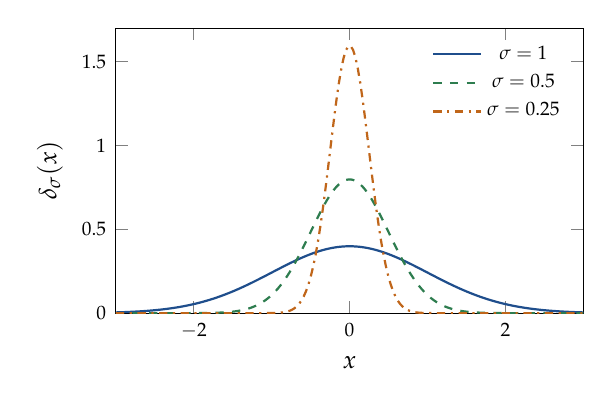
\begin{tikzpicture}
\begin{axis}[width=0.62\linewidth,height=5.2cm,xmin=-3,xmax=3,ymin=0,ymax=1.7,domain=-3:3,samples=200,
  xlabel={$x$},ylabel={$\delta_\sigma(x)$},legend style={font=\scriptsize,draw=none,fill=none},
  tick label style={font=\scriptsize},label style={font=\small}]
\addplot[thick,keyblue]           {exp(-x^2/(2*1^2))/(sqrt(2*pi)*1)};
\addplot[thick,resgreen,dashed]   {exp(-x^2/(2*0.5^2))/(sqrt(2*pi)*0.5)};
\addplot[thick,exorange,dash dot] {exp(-x^2/(2*0.25^2))/(sqrt(2*pi)*0.25)};
\legend{$\sigma=1$,$\sigma=0.5$,$\sigma=0.25$}
\end{axis}
\end{tikzpicture}
\caption{The Gaussian family \eqref{eq:deltagauss}. Every member has unit area; as $\sigma\to0$ the family converges
(inside integrals) to $\delta(x)$. With $\sigma^2=2\kappa t$ the same curves are snapshots of a diffusing spike.}
\label{fig:deltaseq}
\end{figure}

\begin{center}
\small
\renewcommand{\arraystretch}{1.3}
\begin{tabularx}{\linewidth}{@{}l>{$\displaystyle}l<{$}X@{}}
\toprule
& \text{Property} & Remark \\ \midrule
\textcolor{srcpurple}{(B.4.2)} & x\,\delta(x-a)=a\,\delta(x-a) & multiply by the value at the spike \\
\textcolor{srcpurple}{(B.4.3)} & \int_a^b\delta(x-x_0)\,dx=\begin{cases}1,& a\le x_0\le b\\0,& x_0<a\text{ or }x_0>b\end{cases} & strictly, a spike exactly on a limit gives $\tfrac12$ with symmetric definitions --- avoid it \\
\textcolor{srcpurple}{(B.4.4)} & \int_{-\infty}^{\infty}f(x)\,\delta(x-x_0)\,dx=f(x_0) & sifting \\
 & \delta(\alpha x)=\delta(x)/|\alpha| & scaling (change variables in the integral) \\
 & \delta\big(g(x)\big)=\sum_n\frac{\delta(x-x_n)}{|g'(x_n)|} & $x_n$ = simple roots of $g$ \\
 & \int f(x)\,\delta'(x-x_0)\,dx=-f'(x_0) & integrate by parts \\
 & H'(x)=\delta(x),\quad \int_{-\infty}^{x}\delta(s)\,ds=H(x) & step $\leftrightarrow$ spike \\
 & [\delta(x)]=[x]^{-1},\quad [\delta(\xx)]=[\text{volume}]^{-1} & a point source $Q\,\delta(\xx-\xx_0)$ has units of $Q$ per volume \\
\bottomrule
\end{tabularx}
\end{center}

In three dimensions $\delta(\xx-\xx_0)=\delta(x-x_0)\,\delta(y-y_0)\,\delta(z-z_0)$ \citep[p.~892]{kundu2016}. In curvilinear
coordinates the rule $\int\delta(\xx-\xx_0)\,dV=1$ forces division by the scale factors of Section~\ref{sec:B5}:
\begin{equation}\label{eq:deltacurv}
\delta(\xx-\xx_0)=\frac{\delta(R-R_0)\,\delta(\varphi-\varphi_0)\,\delta(z-z_0)}{R_0}
=\frac{\delta(r-r_0)\,\delta(\theta-\theta_0)\,\delta(\varphi-\varphi_0)}{r_0^2\sin\theta_0}.
\end{equation}
A line source of strength $m$ per unit length on the $z$-axis is $m\,\delta(x)\delta(y)=m\,\delta(R)/(2\pi R)$, with the
one-sided convention $\int_0^\infty\delta(R)\,dR=1$.

\begin{pitfall}[one symbol, three meanings]
In fluid mechanics $\delta$ is also a boundary-layer thickness or another length scale \citep[p.~892]{kundu2016}, and
$\delta_{ij}$ is the Kronecker delta.
A second trap is the units: $\delta(x)$ is \emph{not} dimensionless. A sediment source $I\,\delta(x-x_0)$ in a 1D river model has
units of $I$ per metre.
\end{pitfall}

\begin{worked}[Example B.4 revisited: a moving source]\label{we:B4}
Evaluate $I=\int_{-\infty}^{+\infty}F(x)\,[(x_0-x)^2+r_0^2]^{-1/2}\,e^{ikx}\,\delta(x-ct)\,dx$.

The integration variable is $x$; time $t$ is a parameter. The spike sits at $x=ct$, which always lies inside $(-\infty,\infty)$,
so \eqref{eq:sifting} simply replaces $x$ by $ct$:
\[
I=F(ct)\,[(x_0-ct)^2+r_0^2]^{-1/2}\,e^{ikct}.
\]
Physically, $\delta(x-ct)$ describes a point source moving at speed $c$ (a ship, a moving load, a migrating bar front); the
integral ``samples'' the rest of the integrand at the source's instantaneous position.
\end{worked}

\subsection{Green's functions: responses to impulses}
Suppose $f$ obeys a linear equation $\mathcal L f=s$ with a source $s(x,t)$. Because any source can be written as a
superposition of impulses,
$s(x,t)=\iint s(\xi,\tau)\,\delta(x-\xi)\,\delta(t-\tau)\,d\xi\,d\tau$ by \eqref{eq:sifting}, the response to a unit impulse,
$\mathcal L G=\delta(x-\xi)\,\delta(t-\tau)$, builds every other response:
\begin{equation}\label{eq:green}
f(x,t)=\iint G(x,t;\xi,\tau)\,s(\xi,\tau)\,d\xi\,d\tau\qquad(+\ \text{initial and boundary terms}).
\end{equation}
For diffusion on an infinite line, $\partial c/\partial t=\kappa\,\partial^2c/\partial x^2$ with $c(x,0)=\delta(x)$, the impulse response is
\begin{equation}\label{eq:heatkernel}
G(x,t)=\frac{1}{\sqrt{4\pi\kappa t}}\exp\!\left(-\frac{x^2}{4\kappa t}\right)=\delta_\sigma(x)\quad\text{with}\quad\sigma^2=2\kappa t ,
\end{equation}
exactly Kundu's Gaussian \eqref{eq:deltagauss}. A delta function is a diffusion kernel at $t=0$, and diffusion spreads a spike
into a Gaussian whose variance grows as $2\kappa t$. For any initial condition, $c(x,t)=\int G(x-\xi,t)\,c_0(\xi)\,d\xi$ (a
convolution).

\begin{keyidea}[three routes to the same solution]
The erf solution \eqref{eq:erfsol} can be obtained (i) from a similarity variable (Section~\ref{sec:B2}), (ii) by convolving the
step with $G$ (Exercise~\ref{ex:kernel}), or (iii) by Fourier transform. Seeing the same answer three ways is the best check
that you have understood all three tools.
\end{keyidea}

\subsection{Research connection: impulses and responses in Earth-surface systems}
\begin{research}[tracers, hydrographs, pulses and grains]
\begin{itemize}[leftmargin=1.2em]
  \item \textbf{Tracer injections.} A slug of mass $M$ released at $x=0$ in a channel of cross-section $A$ spreads as
        $c=(M/A)\,(4\pi K_xt)^{-1/2}\exp[-(x-Ut)^2/(4K_xt)]$, the Green's function of advection--dispersion in a moving
        frame (Exercise~\ref{ex:galilean}). The centroid moves at $U$ and the variance grows as $\sigma^2=2K_xt$, so the
        longitudinal dispersion coefficient is $K_x=\tfrac12\,d\sigma^2/dt$ \citep{fischer1979}.
  \item \textbf{Unit hydrographs.} Treating a catchment as a linear system, discharge is the convolution
        $Q(t)=\int_0^tu(t-\tau)\,p(\tau)\,d\tau$ of effective rainfall $p$ with the instantaneous unit hydrograph $u$, the
        response to $p=\delta(t)$. The geomorphological IUH derives $u(t)$ from channel-network structure
        \citep{rodriguez1979}.
  \item \textbf{Sediment pulses.} Landslides and dam removals inject sediment almost impulsively; whether the pulse
        translates downstream or disperses in place is a question about the Green's function of the morphodynamic equations
        \citep{lisle2001}.
  \item \textbf{Signals and shredding.} A storm sequence $\sum_ia_i\,\delta(t-t_i)$ passed through a linear landscape emerges
        as $\sum_ia_i\,G(t-t_i)$: a smoothed and lagged copy. Threshold-dominated, nonlinear transport can instead
        ``shred'' environmental signals \citep{jerolmack2010}, a central theme of complex-systems geomorphology.
  \item \textbf{From grains to fields.} Grains at positions $x_p(t)$ have number density $n(x,t)=\sum_p\delta(x-x_p(t))$.
        Coarse-graining with the Gaussian \eqref{eq:deltagauss}, $n_\sigma=\sum_p\delta_\sigma(x-x_p)$, gives a smooth
        field, and particle motion then implies a continuum conservation law (Exercise~\ref{ex:coarse}) --- the bridge between
        particle or cellular models \citep{murray1994} and Exner-type continuum equations \citep{furbish2012}.
\end{itemize}
\end{research}

\begin{pycode}[the sifting property as $\sigma\to0$]
import numpy as np
x = np.linspace(-20, 20, 400001); dx = x[1] - x[0]
f = lambda x: np.cos(x) + x**2          # any smooth test function
x0 = 1.3
for sig in [1.0, 0.3, 0.1, 0.03]:
    d = np.exp(-(x - x0)**2/(2*sig**2))/(np.sqrt(2*np.pi)*sig)  # (B.4.1)
    area, sift = np.sum(d)*dx, np.sum(f(x)*d)*dx
    print(f"sigma={sig:4.2f}: int(d)={area:.6f}, int(f*d)={sift:.6f}")
print(f"f(x0) = {f(x0):.6f}")
# -> sigma=1.00: int(d)=1.000000, int(f*d)=2.852246
# -> sigma=0.30: int(d)=1.000000, int(f*d)=2.035728
# -> sigma=0.10: int(d)=1.000000, int(f*d)=1.966165
# -> sigma=0.03: int(d)=1.000000, int(f*d)=1.958278
# -> f(x0) = 1.957499  (exact: int(f*d) = exp(-sig^2/2) cos(x0) + x0^2 + sig^2)
\end{pycode}

\begin{remember}
\begin{itemize}
  \item $\delta$ is defined by its action in integrals: unit area, zero width. Sifting picks the value at the spike.
  \item $\delta(\alpha x)=\delta(x)/|\alpha|$; $\delta(x)$ has units of $1/[x]$; in curvilinear coordinates divide by the scale factors.
  \item A Green's function is the response to an impulse; superposition gives every solution of a linear problem.
  \item The diffusion kernel is a spreading delta with variance $2\kappa t$ --- the basis of tracer tests.
\end{itemize}
\end{remember}

\subsection*{Exercises for Section~\ref{sec:B4}}

\begin{exercise}[Integrals with deltas]{1}{deltaint}
Evaluate:
(a) $\int_{-\infty}^{\infty}(x^3+2)\,\delta(x-1)\,dx$;\;
(b) $\int_0^5\cos(\pi x)\,\delta(x-2)\,dx$;\;
(c) $\int_0^5\cos(\pi x)\,\delta(x+2)\,dx$;\;
(d) $\int_{-\infty}^{\infty}e^{x}\,\delta(2x+4)\,dx$;\;
(e) $\int_{-\infty}^{\infty}f(x)\,\delta'(x-a)\,dx$;\;
(f) $\int_{-\infty}^{\infty}\delta(x^2-4)\,dx$.
\end{exercise}

\begin{exercise}[Properties from the Gaussian limit]{1}{deltaprops}
(a) Show that $\int_{-\infty}^\infty\delta_\sigma(x)\,dx=1$ for every $\sigma>0$ and that $\delta_\sigma(x)\to0$ for every fixed
$x\neq0$ as $\sigma\to0$.
(b) Prove $\delta(\alpha x)=\delta(x)/|\alpha|$ by changing variables in $\int f(x)\,\delta(\alpha x)\,dx$.
(c) A 1D Exner equation for a river of width $B$ reads $(1-\lambda_p)\,\partial z_b/\partial t+\partial q_s/\partial x=I\,\delta(x-x_0)$,
with $q_s$ the volumetric bedload flux per unit width ($\mathrm{m^2\,s^{-1}}$). What are the units of $I$, and how is $I$ related
to the volumetric rate $Q_{\mathrm{in}}$ ($\mathrm{m^3\,s^{-1}}$) at which a tributary delivers grains at $x_0$?
\end{exercise}

\begin{exercise}[The diffusion kernel]{2}{kernel}
(a) Verify that $G$ in \eqref{eq:heatkernel} solves $\partial c/\partial t=\kappa\,\partial^2c/\partial x^2$ for $t>0$, has unit area, and has
variance $\int x^2G\,dx=2\kappa t$.
(b) Show that convolving $G$ with the step $c_0(x)=a\sgn(x)$ reproduces $a\erf\big(x/\sqrt{4\kappa t}\big)$.
\end{exercise}

\begin{exercise}[A salt-slug tracer test]{2}{tracer}
$M=5\units{kg}$ of salt is released instantaneously across a river of cross-sectional area $A=20\units{m^2}$. Longitudinal
concentration profiles measured $10$ and $30$ minutes later have centroids at $720\units{m}$ and $2160\units{m}$ and variances
$400\units{m^2}$ and $1600\units{m^2}$.
(a) Estimate the mean velocity $U$ and the dispersion coefficient $K_x$.
(b) Predict the peak concentration at $t=30\units{min}$ (in $\mathrm{mg\,L^{-1}}$ above background).
\end{exercise}

\begin{exercise}[A linear-reservoir unit hydrograph]{2}{hydrograph}
A catchment is modelled as a linear reservoir: storage $V$ obeys $dV/dt=p(t)-Q$, with $Q=V/k$.
(a) Show that the instantaneous unit hydrograph (response to $p=\delta(t)$, with $V(0^-)=0$) is $u(t)=k^{-1}e^{-t/k}H(t)$.
(b) Two storms deliver $p(t)=P_1\delta(t)+P_2\delta(t-t_2)$. Write $Q(t)$ by superposition and evaluate $Q(0^+)$ and
$Q(t_2^+)$ for $k=5\units{h}$, $P_1=20\units{mm}$, $P_2=10\units{mm}$ and $t_2=3\units{h}$.
(c) Why is an instantaneous jump in $Q$ unrealistic, and how does a cascade of reservoirs fix it?
\end{exercise}

\begin{exercise}[Point and line sources in polar coordinates]{2}{polardelta}
(a) Show that in plane polar coordinates a unit point source at $(r_0,\theta_0)$ is $\delta(r-r_0)\,\delta(\theta-\theta_0)/r_0$.
(b) A fully penetrating well pumps $Q$ (volume per time) from a confined aquifer of thickness $b$. Write the sink term per
unit volume, and use the divergence theorem on a cylinder of radius $R$ to show that, at steady state, the radial Darcy flux is
$q_R=-Q/(2\pi bR)$ (toward the well).
\end{exercise}

\begin{exercise}[From particles to a continuum conservation law]{3}{coarse}
Grains move along a line with positions $x_p(t)$ and velocities $v_p=dx_p/dt$.
(a) Show that the smoothed number density $n_\sigma(x,t)=\sum_p\delta_\sigma(x-x_p(t))$ satisfies
$\partial n_\sigma/\partial t+\partial J_\sigma/\partial x=0$ with the flux $J_\sigma=\sum_pv_p\,\delta_\sigma(x-x_p(t))$.
(b) Interpret $J_\sigma/n_\sigma$. How would you choose $\sigma$ when converting particle-tracking data of bedload into an
Exner-type description?
(c) What additional term appears if grains can also be entrained from, or deposited onto, the bed?
\end{exercise}

\clearpage
% =====================================================================
\section{Common Three-Dimensional Coordinate Systems}\label{sec:B5}
% =====================================================================
\begin{source}
\textbf{In your PDF:} \Kundu\ \S B.5, pp.~892--895 --- Cartesian, cylindrical and spherical coordinates: position, unit
vectors, unit-vector derivatives, gradient, and surface and volume integrals (Figs.~B.1--B.3).
\end{source}

\begin{goals}
\begin{itemize}
  \item Derive unit vectors, scale factors and line, area and volume elements from $\xx(q_1,q_2,q_3)$.
  \item Understand why curvilinear unit vectors change with position, and compute their derivatives.
  \item Set up surface and volume integrals in cylindrical and spherical coordinates.
  \item Use spherical geometry correctly on a round Earth.
\end{itemize}
\end{goals}

\subsection{One idea behind all three systems: scale factors}
Write the position as $\xx(q_1,q_2,q_3)$. Changing $q_i$ by $dq_i$ moves the point by $(\partial\xx/\partial q_i)\,dq_i$, so
we define the \emph{scale factor} and the unit vector
\begin{equation}\label{eq:scalefactor}
h_i=\left|\pd{\xx}{q_i}\right|,\qquad \e{i}=\frac{1}{h_i}\pd{\xx}{q_i}.
\end{equation}
For orthogonal systems ($\e{i}\cdot\e{j}=\delta_{ij}$) everything else follows:
\begin{equation}\label{eq:elements}
\begin{gathered}
ds^2=h_1^2dq_1^2+h_2^2dq_2^2+h_3^2dq_3^2,\qquad dA_{(1)}=h_2h_3\,dq_2\,dq_3,\\
dV=h_1h_2h_3\,dq_1dq_2dq_3,\qquad \nabla=\sum_i\frac{\e{i}}{h_i}\pd{}{q_i},
\end{gathered}
\end{equation}
where $dA_{(1)}$ is the area element on a surface $q_1=\text{const}$.

\begin{center}
\small
\renewcommand{\arraystretch}{1.3}
\begin{tabular}{@{}lllll@{}}
\toprule
System & Coordinates & Position & $(h_1,h_2,h_3)$ & $dV$ \\ \midrule
Cartesian & $(x,y,z)$ & $\xx=x\e{x}+y\e{y}+z\e{z}$ & $(1,1,1)$ & $dx\,dy\,dz$ \\
Cylindrical & $(R,\varphi,z)$ & $x=R\cos\varphi,\ y=R\sin\varphi,\ z=z$ & $(1,R,1)$ & $R\,dR\,d\varphi\,dz$ \\
Spherical & $(r,\theta,\varphi)$ & $x=r\sin\theta\cos\varphi,\ y=r\sin\theta\sin\varphi,\ z=r\cos\theta$ & $(1,r,r\sin\theta)$ & $r^2\sin\theta\,dr\,d\theta\,d\varphi$ \\
\bottomrule
\end{tabular}
\end{center}

\begin{worked}[spherical unit vectors and scale factors from the position vector]\label{we:sphscale}
Differentiate $\xx=r(\sin\theta\cos\varphi,\ \sin\theta\sin\varphi,\ \cos\theta)$:
\begin{gather*}
\pd{\xx}{r}=(\sin\theta\cos\varphi,\ \sin\theta\sin\varphi,\ \cos\theta),\qquad
\pd{\xx}{\theta}=r\,(\cos\theta\cos\varphi,\ \cos\theta\sin\varphi,\ -\sin\theta),\\
\pd{\xx}{\varphi}=r\sin\theta\,(-\sin\varphi,\ \cos\varphi,\ 0).
\end{gather*}
The magnitudes are $h_r=1$, $h_\theta=r$ and $h_\varphi=r\sin\theta$, and dividing by them gives exactly \Kundu's unit
vectors (p.~894):
$\e{r}=\e{x}\sin\theta\cos\varphi+\e{y}\sin\theta\sin\varphi+\e{z}\cos\theta$,
$\e{\theta}=\e{x}\cos\theta\cos\varphi+\e{y}\cos\theta\sin\varphi-\e{z}\sin\theta$,
$\e{\varphi}=-\e{x}\sin\varphi+\e{y}\cos\varphi$. The three are mutually orthogonal, so \eqref{eq:elements} applies:
$dV=r^2\sin\theta\,dr\,d\theta\,d\varphi$ and $\nabla=\e{r}\partial_r+\e{\theta}r^{-1}\partial_\theta+\e{\varphi}(r\sin\theta)^{-1}\partial_\varphi$.
\end{worked}

\subsection{Unit vectors that turn}
In Cartesian coordinates the unit vectors are the same everywhere, $\partial\e{i}/\partial x_j=0$. In curvilinear coordinates
they are not \citep[pp.~893--894]{kundu2016}:
\begin{align}
&\text{cylindrical:} && \pd{\e{R}}{\varphi}=\e{\varphi},\qquad \pd{\e{\varphi}}{\varphi}=-\e{R},\qquad\text{all other derivatives zero;}\label{eq:cylderiv}\\
&\text{spherical:} && \pd{\e{r}}{\theta}=\e{\theta},\ \ \pd{\e{r}}{\varphi}=\sin\theta\,\e{\varphi},\ \
\pd{\e{\theta}}{\theta}=-\e{r},\ \ \pd{\e{\theta}}{\varphi}=\cos\theta\,\e{\varphi},\ \
\pd{\e{\varphi}}{\varphi}=-\sin\theta\,\e{r}-\cos\theta\,\e{\theta},\label{eq:sphderiv}
\end{align}
with all $r$-derivatives and $\partial\e{\varphi}/\partial\theta$ equal to zero. Geometrically, moving through an angle $d\varphi$ at
fixed $R$ rotates the pair $(\e{R},\e{\varphi})$ rigidly by $d\varphi$ (\cref{fig:coords}b), so $d\e{R}=\e{\varphi}\,d\varphi$ and
$d\e{\varphi}=-\e{R}\,d\varphi$.

\begin{figure}[htbp]
\centering
\tdplotsetmaincoords{70}{110}
\begin{tikzpicture}[tdplot_main_coords,>=Latex,line cap=round]
\def\Th{35}\def\Ph{55}\def\Rr{2.4}
\coordinate (O) at (0,0,0);
\draw[->] (O) -- (3.0,0,0) node[anchor=north east]{$x$};
\draw[->] (O) -- (0,3.0,0) node[anchor=north west]{$y$};
\draw[->] (O) -- (0,0,3.0) node[anchor=south]{$z$};
\coordinate (P) at ({\Rr*sin(\Th)*cos(\Ph)},{\Rr*sin(\Th)*sin(\Ph)},{\Rr*cos(\Th)});
\coordinate (Pxy) at ({\Rr*sin(\Th)*cos(\Ph)},{\Rr*sin(\Th)*sin(\Ph)},0);
\draw[thick,->] (O) -- (P) node[pos=0.55,left=1pt]{$r$};
\draw[dashed,gray] (O) -- (Pxy) -- (P);
\tdplotdrawarc{(O)}{0.8}{0}{\Ph}{anchor=north}{$\varphi$}
\tdplotsetthetaplanecoords{\Ph}
\tdplotdrawarc[tdplot_rotated_coords]{(0,0,0)}{0.75}{0}{\Th}{anchor=south west}{$\theta$}
\fill (P) circle (1.2pt);
\draw[->,pitred,very thick] (P) -- ++({0.9*sin(\Th)*cos(\Ph)},{0.9*sin(\Th)*sin(\Ph)},{0.9*cos(\Th)}) node[anchor=south]{$\e{r}$};
\draw[->,resgreen,very thick] (P) -- ++({0.9*cos(\Th)*cos(\Ph)},{0.9*cos(\Th)*sin(\Ph)},{-0.9*sin(\Th)}) node[anchor=north west]{$\e{\theta}$};
\draw[->,keyblue,very thick] (P) -- ++({-0.9*sin(\Ph)},{0.9*cos(\Ph)},0) node[anchor=west]{$\e{\varphi}$};
\node[font=\small] at (1.8,-1.2,2.9) {(a)};
\end{tikzpicture}
\hspace{1.2cm}
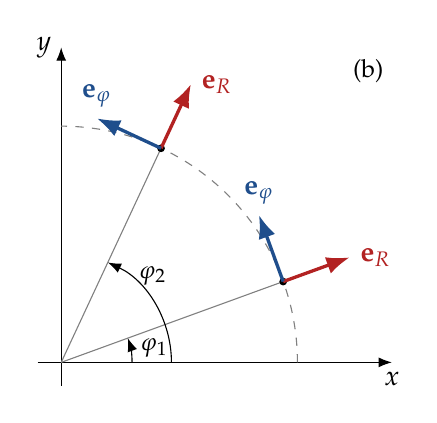
\begin{tikzpicture}[>=Latex,scale=1.0]
\draw[->] (-0.3,0) -- (4.2,0) node[below]{$x$};
\draw[->] (0,-0.3) -- (0,4.0) node[left]{$y$};
\draw[gray,dashed] (3,0) arc (0:90:3);
\foreach \ang/\lab in {20/1,65/2}{
  \coordinate (Q) at (\ang:3);
  \draw[gray] (0,0) -- (Q);
  \fill (Q) circle (1.4pt);
  \draw[->,pitred,very thick] (Q) -- ++(\ang:0.9) node[anchor=west]{$\e{R}$};
  \draw[->,keyblue,very thick] (Q) -- ++(\ang+90:0.9) node[anchor=south]{$\e{\varphi}$};
}
\draw[->,thin] (0.9,0) arc (0:20:0.9) node[pos=0.6,right]{\small$\varphi_1$};
\draw[->,thin] (1.4,0) arc (0:65:1.4) node[pos=0.8,right]{\small$\varphi_2$};
\node[font=\small] at (3.9,3.7) {(b)};
\end{tikzpicture}
\caption{(a) Spherical coordinates in \Kundu's convention: $\theta$ is measured from the $+z$ axis (co-latitude) and
$\varphi$ is the azimuth; the local unit vectors $\e{r},\e{\theta},\e{\varphi}$ form a right-handed orthonormal triad that changes
from point to point. (b) Cylindrical (or plane polar) unit vectors at two azimuths: the pair $(\e{R},\e{\varphi})$ rotates
rigidly with $\varphi$, which is the origin of \eqref{eq:cylderiv}.}
\label{fig:coords}
\end{figure}

\begin{pitfall}[conventions and notation]
\begin{itemize}[leftmargin=1.2em]
  \item \Kundu\ (like most physics and engineering texts) uses $\theta$ for the polar angle and $\varphi$ for the azimuth; many
        mathematics texts swap them. Geoscience uses latitude $\vartheta=90^\circ-\theta$ and longitude $\lambda=\varphi$.
        Always check before copying a formula.
  \item \Kundu\ writes $R$ for the cylindrical radius and $r$ for the spherical radius; in plane polar coordinates
        (\S B.6) he uses $(r,\theta)$, where $\theta$ plays the role of the cylindrical $\varphi$.
  \item Typo alert: on pp.~893--894 some cylindrical surface and volume integrals are labelled $f(R,\theta,z)$; read
        $\theta$ as the azimuth $\varphi$.
  \item Curvilinear components of a \emph{constant} vector vary with position, e.g.\ $\e{x}=\cos\varphi\,\e{R}-\sin\varphi\,\e{\varphi}$.
\end{itemize}
\end{pitfall}

\begin{worked}[acceleration in cylindrical coordinates]\label{we:cylaccel}
Write $\uu=u_R\e{R}+u_\varphi\e{\varphi}+u_z\e{z}$ and follow a fluid particle. Its azimuth changes at the rate
$D\varphi/Dt=u_\varphi/R$, so by \eqref{eq:cylderiv}
$D\e{R}/Dt=(\partial\e{R}/\partial\varphi)\,D\varphi/Dt=(u_\varphi/R)\,\e{\varphi}$ and $D\e{\varphi}/Dt=-(u_\varphi/R)\,\e{R}$. Therefore
\begin{equation}\label{eq:cylaccel}
\Dt{\uu}=\left(\Dt{u_R}-\frac{u_\varphi^2}{R}\right)\e{R}+\left(\Dt{u_\varphi}+\frac{u_Ru_\varphi}{R}\right)\e{\varphi}+\Dt{u_z}\,\e{z}.
\end{equation}
$-u_\varphi^2/R$ is the centripetal acceleration and $u_Ru_\varphi/R$ expresses angular-momentum conservation (a parcel moving inward
spins up). These are exactly the ``extra'' terms of the cylindrical Navier--Stokes equations in \S B.6: they come from geometry,
not from new forces.
\end{worked}

\subsection{Surface and volume integrals}
\Kundu\ lists the integrals on pp.~893--895. They all follow one rule: on a coordinate surface, the area element is the product of
the two scale factors of the coordinates that vary on it.
\begin{center}
\small
\renewcommand{\arraystretch}{1.3}
\begin{tabular}{@{}lll@{}}
\toprule
System & Surface & Element \\ \midrule
Cartesian & plane $x=\xi$ / $y=\psi$ / $z=\zeta$ & $dy\,dz$ \ / \ $dz\,dx$ \ / \ $dx\,dy$ \\
Cylindrical & cylinder $R=\xi$; half-plane $\varphi=\psi$; plane $z=\zeta$ & $\xi\,d\varphi\,dz$; \ $dR\,dz$; \ $R\,dR\,d\varphi$ \\
Spherical & sphere $r=\xi$; cone $\theta=\psi$; half-plane $\varphi=\zeta$ & $\xi^2\sin\theta\,d\theta\,d\varphi$; \ $r\sin\psi\,dr\,d\varphi$; \ $r\,dr\,d\theta$ \\
\bottomrule
\end{tabular}
\end{center}

\begin{worked}[volumes of simple landforms]\label{we:volumes}
A volcanic cone of height $H$ and basal radius $R_b$ has $z=H(1-R/R_b)$, so
$V=\int_0^{2\pi}\!\int_0^{R_b}H(1-R/R_b)\,R\,dR\,d\varphi=2\pi H\left(\tfrac12R_b^2-\tfrac13R_b^2\right)=\tfrac13\pi R_b^2H$.
A Gaussian hill $z=He^{-R^2/\ell^2}$ has $V=2\pi H\int_0^\infty e^{-R^2/\ell^2}R\,dR=\pi\ell^2H$.
Forgetting the factor $R$ in $R\,dR\,d\varphi$ is the most common error in such integrals.
\end{worked}

\subsection{Research connection: a round planet and radial landforms}
\begin{research}[spherical areas, fans and rotation]
\begin{itemize}[leftmargin=1.2em]
  \item \textbf{Area on the sphere.} With latitude $\vartheta=90^\circ-\theta$, the area element is
        $dA=R_E^2\sin\theta\,d\theta\,d\varphi=R_E^2\cos\vartheta\,d\vartheta\,d\lambda$. A cell spanning $\Delta\lambda$ between
        latitudes $\vartheta_1$ and $\vartheta_2$ has area $R_E^2\,\Delta\lambda\,(\sin\vartheta_2-\sin\vartheta_1)$: a $1^\circ\times1^\circ$
        cell at $36^\circ$N (Durham, NC) covers about $10\,000\units{km^2}$, only $81\%$ of an equatorial cell. Global statistics on
        latitude--longitude grids (erosion rates, sediment yields, precipitation) must therefore be area-weighted.
  \item \textbf{Radial landforms and experiments.} Alluvial fans, deltas, volcanoes, craters, pumping wells, rotating tanks and
        annular flumes are natural in cylindrical coordinates. The factor $R$ in the area element changes the physics: a sediment
        flux spreading radially is diluted as $1/R$, and diffusive domes are half as high as ridges of the same width
        (Exercise~\ref{ex:dome}).
  \item \textbf{Rotation.} The Coriolis parameter $f=2\Omega\sin\vartheta$ is \emph{twice} the local-vertical component of Earth's rotation
        vector $\Omega\,\e{z}$: $f=2\bm\Omega\cdot\e{r}=2\Omega\cos\theta$. It matters for large rivers, lakes and coastal flows.
\end{itemize}
\end{research}

\begin{pycode}[areas of latitude--longitude cells]
import numpy as np
R = 6371.0                               # mean Earth radius [km]
def cell_area(lat1, lat2, dlon):         # degrees -> km^2
    """Area of a lat-lon cell: integral of R^2 cos(lat) dlat dlon."""
    s1, s2 = np.sin(np.radians(lat1)), np.sin(np.radians(lat2))
    return R**2*np.radians(dlon)*(s2 - s1)
print(f"{cell_area(-0.5, 0.5, 1.0):.0f} km^2 at the equator")  # -> 12364
print(f"{cell_area(35.5, 36.5, 1.0):.0f} km^2 at 36 N")        # -> 10003
lat = np.arange(-90.0, 90.0, 1.0)        # all 1-degree latitude bands
total = 360*cell_area(lat, lat + 1, 1.0).sum()
print(f"{total:.4e} vs 4 pi R^2 = {4*np.pi*R**2:.4e}")  # -> 5.1006e+08 (both)
\end{pycode}

\begin{remember}
\begin{itemize}
  \item $h_i=|\partial\xx/\partial q_i|$, $\e{i}=h_i^{-1}\partial\xx/\partial q_i$, $dV=h_1h_2h_3\,dq_1dq_2dq_3$, $\nabla=\sum_i\e{i}h_i^{-1}\partial_{q_i}$.
  \item Scale factors: Cartesian $(1,1,1)$, cylindrical $(1,R,1)$, spherical $(1,r,r\sin\theta)$.
  \item Curvilinear unit vectors turn with position; their derivatives produce centripetal and angular-momentum terms.
  \item On the sphere, area scales with $\cos(\text{latitude})$: weight global averages accordingly.
\end{itemize}
\end{remember}

\subsection*{Exercises for Section~\ref{sec:B5}}

\begin{exercise}[Cylindrical unit vectors from scratch]{1}{cylunit}
From $\xx=(R\cos\varphi,R\sin\varphi,z)$ and \eqref{eq:scalefactor}, derive $h_R$, $h_\varphi$, $h_z$ and the unit vectors
$\e{R},\e{\varphi},\e{z}$; check that they are orthonormal and verify \eqref{eq:cylderiv}.
\end{exercise}

\begin{exercise}[Spherical unit-vector derivatives]{1}{sphunit}
Using the Cartesian expressions of Worked example~\ref{we:sphscale}, verify $\partial\e{r}/\partial\varphi=\sin\theta\,\e{\varphi}$ and
$\partial\e{\varphi}/\partial\varphi=-\sin\theta\,\e{r}-\cos\theta\,\e{\theta}$. Interpret the second result for a point moving along a circle of
latitude.
\end{exercise}

\begin{exercise}[Acceleration in spherical coordinates]{2}{sphaccel}
Following Worked example~\ref{we:cylaccel}, use $D\theta/Dt=u_\theta/r$, $D\varphi/Dt=u_\varphi/(r\sin\theta)$ and \eqref{eq:sphderiv} to show that
the $r$- and $\theta$-components of $D\uu/Dt$ are $Du_r/Dt-(u_\theta^2+u_\varphi^2)/r$ and $Du_\theta/Dt+u_ru_\theta/r-u_\varphi^2\cot\theta/r$,
in agreement with the spherical Navier--Stokes equations of \Kundu\ \S B.6.
\end{exercise}

\begin{exercise}[Grid cells on a round Earth]{1}{latlon}
(a) Derive the area of a latitude--longitude cell from $dA=R_E^2\cos\vartheta\,d\vartheta\,d\lambda$.
(b) At roughly what latitude is a $1^\circ\times1^\circ$ cell half the area of an equatorial one?
(c) A global erosion map on a $1^\circ$ grid is averaged by giving every cell equal weight. Is the result biased towards
high- or low-latitude values?
\end{exercise}

\begin{exercise}[The volume of a fan-shaped deposit]{2}{fan}
A debris-flow fan occupies a sector of angle $\Theta$ with its apex at $R=0$; its thickness decays downfan as
$T(R)=T_0e^{-R/\ell_d}$.
(a) Show that the deposit volume is $V=\Theta\,T_0\,\ell_d^2$.
(b) Evaluate $V$ for $\Theta=90^\circ$, $T_0=5\units{m}$ and $\ell_d=2\units{km}$.
(c) What fraction of the volume lies within $R<\ell_d$?
\end{exercise}

\begin{exercise}[Where is Earth's surface?]{2}{caps}
(a) Show that the area of the cap poleward of latitude $\vartheta_0$ is $2\pi R_E^2(1-\sin\vartheta_0)$.
(b) What fraction of Earth's surface lies poleward of $60^\circ$N?
(c) Show that exactly half of Earth's surface lies between $30^\circ$S and $30^\circ$N.
\end{exercise}

\clearpage
% =====================================================================
\section{Equations in Curvilinear Coordinates}\label{sec:B6}
% =====================================================================
\begin{source}
\textbf{In your PDF:} \Kundu\ \S B.6, pp.~895--898 --- plane polar, cylindrical and spherical forms of the gradient, Laplacian,
divergence, curl, vector Laplacian, strain rate, continuity and Navier--Stokes equations.
\end{source}

\begin{goals}
\begin{itemize}
  \item Generate any operator in any orthogonal coordinate system from its scale factors, instead of memorising.
  \item Explain where the extra terms of the curvilinear Navier--Stokes equations come from.
  \item Avoid the classic component errors: $[(\uu\cdot\nabla)\uu]_R\neq(\uu\cdot\nabla)u_R$ and $(\nabla^2\uu)_R\neq\nabla^2u_R$.
  \item Solve classic exact flows (vortices, pipe flow, Stokes flow past a sphere) and apply them to meanders, settling grains
        and wells.
\end{itemize}
\end{goals}

\subsection{Master formulas: everything from the scale factors}
For orthogonal coordinates $(q_1,q_2,q_3)$ with scale factors $h_i$ and $H=h_1h_2h_3$,
\begin{align}
\nabla f&=\sum_i\frac{\e{i}}{h_i}\pd{f}{q_i},\qquad
\nabla\cdot\uu=\frac1H\sum_i\pd{}{q_i}\!\left(\frac{H}{h_i}u_i\right),\qquad
\nabla^2 f=\frac1H\sum_i\pd{}{q_i}\!\left(\frac{H}{h_i^2}\pd{f}{q_i}\right),\label{eq:master1}\\
\nabla\times\uu&=\frac1H\det\begin{pmatrix}h_1\e{1}&h_2\e{2}&h_3\e{3}\\ \partial/\partial q_1&\partial/\partial q_2&\partial/\partial q_3\\ h_1u_1&h_2u_2&h_3u_3\end{pmatrix},
\qquad \nabla^2\uu=\nabla(\nabla\cdot\uu)-\nabla\times(\nabla\times\uu).\label{eq:master2}
\end{align}
The last relation, (B.3.13) read backwards, is the only safe definition of the vector Laplacian in curvilinear coordinates.
Every operator in \Kundu\ \S B.6 (gradient, divergence, curl, Laplacian, vector Laplacian) follows from
\eqref{eq:master1}--\eqref{eq:master2} with $(1,r,1)$ for plane polar, $(1,R,1)$ for cylindrical and $(1,r,r\sin\theta)$ for
spherical coordinates; the strain rates and the acceleration terms also need the unit-vector derivatives
\eqref{eq:cylderiv}--\eqref{eq:sphderiv}. All of \Kundu's \S B.6 formulas were checked symbolically for this guide and are
correct as printed.

\begin{worked}[spherical divergence and Laplacian in two lines]\label{we:sphdiv}
With $H=r^2\sin\theta$ and $H/h_i=(r^2\sin\theta,\ r\sin\theta,\ r)$,
\begin{align*}
\nabla\cdot\uu&=\frac{1}{r^2\sin\theta}\left[\pd{(r^2\sin\theta\,u_r)}{r}+\pd{(r\sin\theta\,u_\theta)}{\theta}+\pd{(r\,u_\varphi)}{\varphi}\right]\\
&=\frac{1}{r^2}\pd{(r^2u_r)}{r}+\frac{1}{r\sin\theta}\pd{(u_\theta\sin\theta)}{\theta}+\frac{1}{r\sin\theta}\pd{u_\varphi}{\varphi},
\end{align*}
and with $H/h_i^2=(r^2\sin\theta,\ \sin\theta,\ 1/\sin\theta)$,
\[
\nabla^2\psi=\frac{1}{r^2}\pd{}{r}\!\left(r^2\pd{\psi}{r}\right)+\frac{1}{r^2\sin\theta}\pd{}{\theta}\!\left(\sin\theta\pd{\psi}{\theta}\right)
+\frac{1}{r^2\sin^2\theta}\pdd{\psi}{\varphi},
\]
as on p.~897 of \Kundu.
\end{worked}

\subsection{Reference formulas}
Plane polar coordinates $(r,\theta)$ are the cylindrical formulas with $\partial/\partial z=0$, $u_z=0$ and $(R,\varphi)\to(r,\theta)$; they
are listed separately on p.~895 of \Kundu. The Navier--Stokes equations below are for constant $\rho$ and $\nu$ and no body force; the continuity equation is general, and
$\tau_{ij}=2\mu S_{ij}$ holds for incompressible flow.

\begin{formulabox}[Cylindrical coordinates $(R,\varphi,z)$ \quad \textnormal{(\Kundu\ p.~896)}]
\small
\begin{align*}
&\nabla\psi=\e{R}\pd{\psi}{R}+\frac{\e{\varphi}}{R}\pd{\psi}{\varphi}+\e{z}\pd{\psi}{z},\qquad
\nabla^2\psi=\frac1R\pd{}{R}\!\left(R\pd{\psi}{R}\right)+\frac{1}{R^2}\pdd{\psi}{\varphi}+\pdd{\psi}{z},\\
&\nabla\cdot\uu=\frac1R\pd{(Ru_R)}{R}+\frac1R\pd{u_\varphi}{\varphi}+\pd{u_z}{z},\\
&\bomega=\e{R}\!\left(\frac1R\pd{u_z}{\varphi}-\pd{u_\varphi}{z}\right)+\e{\varphi}\!\left(\pd{u_R}{z}-\pd{u_z}{R}\right)
+\e{z}\!\left(\frac1R\pd{(Ru_\varphi)}{R}-\frac1R\pd{u_R}{\varphi}\right),\\
&\nabla^2\uu=\e{R}\!\left(\nabla^2u_R-\frac{u_R}{R^2}-\frac{2}{R^2}\pd{u_\varphi}{\varphi}\right)
+\e{\varphi}\!\left(\nabla^2u_\varphi+\frac{2}{R^2}\pd{u_R}{\varphi}-\frac{u_\varphi}{R^2}\right)+\e{z}\nabla^2u_z,\\
&S_{RR}=\pd{u_R}{R},\quad S_{\varphi\varphi}=\frac1R\pd{u_\varphi}{\varphi}+\frac{u_R}{R},\quad S_{zz}=\pd{u_z}{z},\quad
S_{R\varphi}=\frac R2\pd{}{R}\!\left(\frac{u_\varphi}{R}\right)+\frac{1}{2R}\pd{u_R}{\varphi},\\
&S_{\varphi z}=\frac{1}{2R}\pd{u_z}{\varphi}+\frac12\pd{u_\varphi}{z},\quad S_{zR}=\frac12\left(\pd{u_R}{z}+\pd{u_z}{R}\right),\\
&\pd{\rho}{t}+\frac1R\pd{(R\rho u_R)}{R}+\frac1R\pd{(\rho u_\varphi)}{\varphi}+\pd{(\rho u_z)}{z}=0,\\
&\pd{u_R}{t}+(\uu\cdot\nabla)u_R-\frac{u_\varphi^2}{R}=-\frac1\rho\pd{p}{R}+\nu\left(\nabla^2u_R-\frac{u_R}{R^2}-\frac{2}{R^2}\pd{u_\varphi}{\varphi}\right),\\
&\pd{u_\varphi}{t}+(\uu\cdot\nabla)u_\varphi+\frac{u_Ru_\varphi}{R}=-\frac{1}{\rho R}\pd{p}{\varphi}+\nu\left(\nabla^2u_\varphi+\frac{2}{R^2}\pd{u_R}{\varphi}-\frac{u_\varphi}{R^2}\right),\\
&\pd{u_z}{t}+(\uu\cdot\nabla)u_z=-\frac1\rho\pd{p}{z}+\nu\nabla^2u_z,\\
&\text{with the scalar operators}\quad \uu\cdot\nabla=u_R\pd{}{R}+\frac{u_\varphi}{R}\pd{}{\varphi}+u_z\pd{}{z}\quad\text{and}\quad\nabla^2\ \text{as above.}
\end{align*}
\end{formulabox}

\begin{formulabox}[Spherical coordinates $(r,\theta,\varphi)$ \quad \textnormal{(\Kundu\ pp.~897--898)}]
\small
\begin{align*}
&\nabla\psi=\e{r}\pd{\psi}{r}+\frac{\e{\theta}}{r}\pd{\psi}{\theta}+\frac{\e{\varphi}}{r\sin\theta}\pd{\psi}{\varphi},\qquad
\nabla\cdot\uu=\frac{1}{r^2}\pd{(r^2u_r)}{r}+\frac{1}{r\sin\theta}\pd{(u_\theta\sin\theta)}{\theta}+\frac{1}{r\sin\theta}\pd{u_\varphi}{\varphi},\\
&\nabla^2\psi=\frac{1}{r^2}\pd{}{r}\!\left(r^2\pd{\psi}{r}\right)+\frac{1}{r^2\sin\theta}\pd{}{\theta}\!\left(\sin\theta\pd{\psi}{\theta}\right)+\frac{1}{r^2\sin^2\theta}\pdd{\psi}{\varphi},\\
&\bomega=\frac{\e{r}}{r\sin\theta}\left(\pd{(u_\varphi\sin\theta)}{\theta}-\pd{u_\theta}{\varphi}\right)
+\frac{\e{\theta}}{r}\left(\frac{1}{\sin\theta}\pd{u_r}{\varphi}-\pd{(ru_\varphi)}{r}\right)
+\frac{\e{\varphi}}{r}\left(\pd{(ru_\theta)}{r}-\pd{u_r}{\theta}\right),\\
&\nabla^2\uu=\e{r}\!\left(\nabla^2u_r-\frac{2u_r}{r^2}-\frac{2}{r^2\sin\theta}\pd{(u_\theta\sin\theta)}{\theta}-\frac{2}{r^2\sin\theta}\pd{u_\varphi}{\varphi}\right)\\
&\hphantom{\nabla^2\uu=}+\e{\theta}\!\left(\nabla^2u_\theta+\frac{2}{r^2}\pd{u_r}{\theta}-\frac{u_\theta}{r^2\sin^2\theta}-\frac{2\cos\theta}{r^2\sin^2\theta}\pd{u_\varphi}{\varphi}\right)\\
&\hphantom{\nabla^2\uu=}+\e{\varphi}\!\left(\nabla^2u_\varphi+\frac{2}{r^2\sin\theta}\pd{u_r}{\varphi}+\frac{2\cos\theta}{r^2\sin^2\theta}\pd{u_\theta}{\varphi}-\frac{u_\varphi}{r^2\sin^2\theta}\right),\\
&S_{rr}=\pd{u_r}{r},\quad S_{\theta\theta}=\frac1r\pd{u_\theta}{\theta}+\frac{u_r}{r},\quad
S_{\varphi\varphi}=\frac{1}{r\sin\theta}\pd{u_\varphi}{\varphi}+\frac{u_r}{r}+\frac{u_\theta\cot\theta}{r},\\
&S_{r\theta}=\frac r2\pd{}{r}\!\left(\frac{u_\theta}{r}\right)+\frac{1}{2r}\pd{u_r}{\theta},\quad
S_{\theta\varphi}=\frac{\sin\theta}{2r}\pd{}{\theta}\!\left(\frac{u_\varphi}{\sin\theta}\right)+\frac{1}{2r\sin\theta}\pd{u_\theta}{\varphi},\quad
S_{\varphi r}=\frac{1}{2r\sin\theta}\pd{u_r}{\varphi}+\frac r2\pd{}{r}\!\left(\frac{u_\varphi}{r}\right),\\
&\pd{\rho}{t}+\frac{1}{r^2}\pd{(\rho r^2u_r)}{r}+\frac{1}{r\sin\theta}\pd{(\rho u_\theta\sin\theta)}{\theta}+\frac{1}{r\sin\theta}\pd{(\rho u_\varphi)}{\varphi}=0,\\
&\pd{u_r}{t}+(\uu\cdot\nabla)u_r-\frac{u_\theta^2+u_\varphi^2}{r}=-\frac1\rho\pd{p}{r}\\
&\qquad\qquad+\nu\left[\nabla^2u_r-\frac{2u_r}{r^2}-\frac{2}{r^2\sin\theta}\pd{(u_\theta\sin\theta)}{\theta}-\frac{2}{r^2\sin\theta}\pd{u_\varphi}{\varphi}\right],\\
&\pd{u_\theta}{t}+(\uu\cdot\nabla)u_\theta+\frac{u_ru_\theta}{r}-\frac{u_\varphi^2\cot\theta}{r}=-\frac{1}{\rho r}\pd{p}{\theta}\\
&\qquad\qquad+\nu\left[\nabla^2u_\theta+\frac{2}{r^2}\pd{u_r}{\theta}-\frac{u_\theta}{r^2\sin^2\theta}-\frac{2\cos\theta}{r^2\sin^2\theta}\pd{u_\varphi}{\varphi}\right],\\
&\pd{u_\varphi}{t}+(\uu\cdot\nabla)u_\varphi+\frac{u_\varphi u_r}{r}+\frac{u_\theta u_\varphi\cot\theta}{r}=-\frac{1}{\rho r\sin\theta}\pd{p}{\varphi}\\
&\qquad\qquad+\nu\left[\nabla^2u_\varphi+\frac{2}{r^2\sin\theta}\pd{u_r}{\varphi}+\frac{2\cos\theta}{r^2\sin^2\theta}\pd{u_\theta}{\varphi}-\frac{u_\varphi}{r^2\sin^2\theta}\right],\\
&\text{with}\quad \uu\cdot\nabla=u_r\pd{}{r}+\frac{u_\theta}{r}\pd{}{\theta}+\frac{u_\varphi}{r\sin\theta}\pd{}{\varphi}.
\end{align*}
\end{formulabox}

\subsection{Where do the extra terms come from?}
\begin{keyidea}[extra terms are geometry, not physics]
Every term that has no Cartesian counterpart comes from differentiating unit vectors \eqref{eq:cylderiv}--\eqref{eq:sphderiv}:
\begin{itemize}[leftmargin=1.2em]
  \item in $(\uu\cdot\nabla)\uu$: the centripetal terms $-u_\varphi^2/R$ and $-(u_\theta^2+u_\varphi^2)/r$, the angular-momentum terms
        $u_Ru_\varphi/R$ and $u_ru_\theta/r$, and in spherical coordinates the $\cot\theta$ terms that arise because $\e{\varphi}$
        turns as one moves along a circle of latitude (Worked example~\ref{we:cylaccel}, Exercise~\ref{ex:sphaccel});
  \item in $\nabla^2\uu$: terms such as $-u_R/R^2-(2/R^2)\,\partial u_\varphi/\partial\varphi$.
\end{itemize}
A good sanity check is a flow that is trivial in Cartesian coordinates, such as uniform flow $U\e{x}$: in cylindrical
components all the extra terms must cancel (Exercise~\ref{ex:uniform}).
\end{keyidea}

\begin{pitfall}[components are not operators applied to components]
In \Kundu's notation $(\uu\cdot\nabla)u_R$ is the \emph{scalar} operator $\uu\cdot\nabla$ acting on the function $u_R$; the
$R$-component of the vector $(\uu\cdot\nabla)\uu$ is $(\uu\cdot\nabla)u_R-u_\varphi^2/R$. Likewise $(\nabla^2\uu)_R\neq\nabla^2u_R$. In the
strain rate, $S_{R\varphi}$ contains $(R/2)\,\partial(u_\varphi/R)/\partial R$, not $\tfrac12\partial u_\varphi/\partial R$, so that rigid rotation
is strain-free.
\end{pitfall}

\subsection{Exact solutions as worked examples}
\begin{worked}[rigid rotation versus the potential vortex]\label{we:vortices}
For $u_R=u_z=0$ and $u_\varphi(R)$, the cylindrical box gives $\omega_z=R^{-1}d(Ru_\varphi)/dR$ and $S_{R\varphi}=\tfrac R2\,d(u_\varphi/R)/dR$.
\begin{itemize}[leftmargin=1.2em]
  \item \emph{Rigid rotation} $u_\varphi=\Omega R$: $\omega_z=2\Omega$ and $S_{R\varphi}=0$. Elements rotate without deforming.
  \item \emph{Potential vortex} $u_\varphi=\Gamma/(2\pi R)$: $\omega_z=0$ for $R\neq0$ and $S_{R\varphi}=-\Gamma/(2\pi R^2)$. Elements deform
        without rotating, although they travel in circles.
\end{itemize}
The circulation around any circle centred on the origin is $\oint u_\varphi R\,d\varphi=\Gamma$ for the potential vortex, although its
vorticity is zero everywhere except at $R=0$. Stokes' theorem therefore forces the vorticity to be a spike,
$\omega_z=\Gamma\,\delta(x)\,\delta(y)$ (Exercise~\ref{ex:pointvortex}). A Rankine vortex (rigid core of radius $a$, potential flow outside)
is a common model for dust devils and river eddies.
\end{worked}

\begin{worked}[Hagen--Poiseuille flow in a pipe]\label{we:poiseuille}
Seek steady, fully developed flow $\uu=u_z(R)\,\e{z}$ in a pipe of radius $a$. Continuity is satisfied identically; the $R$- and
$\varphi$-momentum equations give $\partial p/\partial R=\partial p/\partial\varphi=0$, so $p=p(z)$, and the $z$-equation reduces to
\[
0=-\frac{1}{\rho}\od{p}{z}+\frac{\nu}{R}\od{}{R}\!\left(R\od{u_z}{R}\right).
\]
The first term depends on $z$ only and the second on $R$ only, so both are constant: $dp/dz=-G$. Integrating twice, with $u_z$
finite at $R=0$ and zero at $R=a$,
\begin{equation}\label{eq:poiseuille}
u_z=\frac{G}{4\mu}\,(a^2-R^2),\qquad Q=\int_0^a u_z\,2\pi R\,dR=\frac{\pi Ga^4}{8\mu},\qquad \bar u=\tfrac12u_{\max},\qquad \tau_w=\tfrac12Ga.
\end{equation}
The $a^4$ dependence makes wide pores, root channels and macropores dominate flow through soils, and underlies the Kozeny--Carman
view of permeability.
\end{worked}

\begin{worked}[Stokes flow past a sphere and the settling velocity]\label{we:stokesflow}
For creeping flow ($Re\ll1$) past a sphere of radius $a$ in a uniform stream $U\e{z}$, the axisymmetric ($u_\varphi=0$) solution in
spherical coordinates is
\begin{equation}\label{eq:stokessphere}
\begin{gathered}
u_r=U\cos\theta\left(1-\frac{3a}{2r}+\frac{a^3}{2r^3}\right),\qquad
u_\theta=-U\sin\theta\left(1-\frac{3a}{4r}-\frac{a^3}{4r^3}\right),\\
p-p_\infty=-\frac32\,\frac{\mu aU\cos\theta}{r^2}.
\end{gathered}
\end{equation}
It satisfies continuity and the Stokes equations $\nabla p=\mu\nabla^2\uu$ --- checked below using exactly the spherical divergence and
vector Laplacian from the box above --- with no slip at $r=a$ and uniform flow as $r\to\infty$. Integrating the stresses over the sphere
gives the drag $F_D=6\pi\mu aU=3\pi\mu dU$, one third from pressure and two thirds from viscous shear. Balancing it against the
submerged weight of a grain, $\tfrac{\pi}{6}(\rho_s-\rho)gd^3$, gives Stokes' settling law
\begin{equation}\label{eq:stokeslaw}
w_s=\frac{R_sgd^2}{18\nu},\qquad R_s=\frac{\rho_s-\rho}{\rho}\approx1.65\ \text{(quartz in water)},
\end{equation}
valid for grain Reynolds numbers $Re_p=w_sd/\nu\lesssim1$.
\end{worked}

\subsection{Research connection: curvature, grains and wells}
\begin{research}[meander bends, suspension, wells and domes]
\textbf{River meanders.} In a bend of radius $R_c$ the dominant balance in the $R$-momentum equation is between the centripetal term
and the pressure gradient, $-u_\varphi^2/R\approx-\rho^{-1}\partial p/\partial R$. With hydrostatic pressure $p=\rho g(\zeta-z)$ this gives a
transverse water-surface slope $\partial\zeta/\partial R\approx u_\varphi^2/(gR)$, i.e.\ a superelevation $\Delta\zeta\approx U^2B/(gR_c)$ across a channel
of width $B$. Because $u_\varphi$ is faster near the surface than near the bed while the pressure gradient is nearly uniform with depth,
near-surface water is driven outward and near-bed water inward: a helical secondary circulation \citep{rozovskii1957} that sweeps
sediment toward the inner bank (point bars) while the outer bank is scoured --- the engine of meander migration
\citep{ikeda1981,seminara2006}; see \cref{fig:meander}.

\textbf{Settling and suspension.} Stokes' law \eqref{eq:stokeslaw} holds for silt and very fine sand; empirical laws extend it to
coarser, natural grains \citep{dietrich1982,ferguson2004}. The settling velocity controls suspension through the Rouse number
$P=w_s/(\kappa_{\mathrm{vK}}u_*)$, which sets the concentration profile $c/c_a=\{[(h-z)/z]\,[a/(h-a)]\}^{P}$ \citep{rouse1937}:
$P\ll1$ gives a nearly uniform profile (wash load), while $P\gtrsim1$ confines sediment near the bed.

\textbf{Wells.} Steady radial flow to a well in a confined aquifer of transmissivity $T$ obeys $r^{-1}d(r\,dh/dr)/dr=0$, so
$h=h_w+(Q/2\pi T)\ln(r/r_w)$ (Thiem). The transient problem has the similarity solution of \citet{theis1935} in the variable
$\eta=r^2S/(4Tt)$ (Exercise~\ref{ex:theis}).

\textbf{Axisymmetric landforms.} Diffusive degradation of cinder cones, domes and crater rims obeys
$\partial z/\partial t=\Up+\kappa R^{-1}\partial(R\,\partial z/\partial R)/\partial R$; the $1/R$ geometry makes their steady forms differ from ridges
(Exercise~\ref{ex:dome}).
\end{research}

\begin{figure}[htbp]
\centering
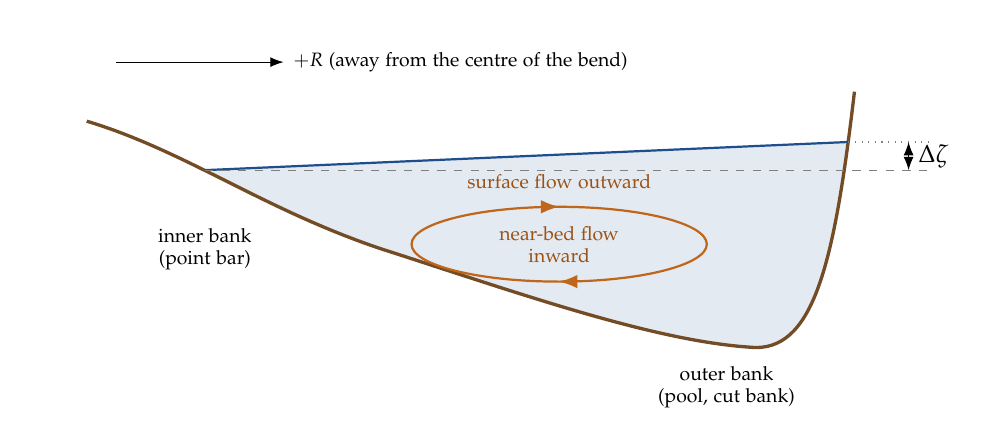
\begin{tikzpicture}[>=Latex,scale=1.25]
\path[use as bounding box] (-0.6,-0.35) rectangle (9.0,3.55);
\def\bed{(0,2.6) .. controls (1.0,2.3) and (1.8,1.7) .. (3.0,1.3) .. controls (4.4,0.85) and (5.8,0.35) .. (6.8,0.3)
          .. controls (7.4,0.3) and (7.6,1.2) .. (7.8,2.9)}
\begin{scope}
  \clip \bed -- (7.8,3.4) -- (0,3.4) -- cycle;
  \fill[keyblue!12] (0,0) -- (0,2.05) -- (8,2.4) -- (8,0) -- cycle;
\end{scope}
\draw[very thick,brown!60!black] \bed;
\draw[thick,keyblue] (1.2,2.1025) -- (7.737,2.3885);
\draw[gray,dashed] (1.2,2.1025) -- (8.55,2.1025);
\draw[gray,dotted] (7.737,2.3885) -- (8.55,2.3885);
\draw[<->] (8.35,2.1025) -- (8.35,2.3885) node[midway,right]{\small$\Delta\zeta$};
\draw[thick,exorange,decoration={markings,mark=at position 0.25 with {\arrow{Latex}},mark=at position 0.75 with {\arrow{Latex}}},
      postaction={decorate}] (6.3,1.35) arc[start angle=0,end angle=-360,x radius=1.5,y radius=0.38];
\node[font=\scriptsize,exorange!80!black] at (4.8,1.99) {surface flow outward};
\node[font=\scriptsize,exorange!80!black,align=center] at (4.8,1.35) {near-bed flow\\inward};
\node[font=\scriptsize,align=center] at (1.2,1.3) {inner bank\\(point bar)};
\node[font=\scriptsize,align=center] at (6.5,-0.1) {outer bank\\(pool, cut bank)};
\draw[->] (0.3,3.2) -- (2.0,3.2) node[right,font=\scriptsize]{$+R$ (away from the centre of the bend)};
\end{tikzpicture}
\caption{Cross-section of a meander bend (vertical scale exaggerated). The centripetal acceleration is balanced on average by a
transverse water-surface slope (superelevation $\Delta\zeta$); the imbalance between the depth-varying centripetal term and the
depth-uniform pressure gradient drives a helical secondary flow that builds point bars on the inner bank.}
\label{fig:meander}
\end{figure}

\begin{pycode}[Stokes flow with \Kundu's spherical formulas, and settling velocities]
import sympy as sp
r, th, a, U, mu = sp.symbols('r theta a U mu', positive=True)
s, c = sp.sin(th), sp.cos(th)
ur = U*c*(1 - 3*a/(2*r) + a**3/(2*r**3))     # Stokes flow past a sphere
ut = -U*s*(1 - 3*a/(4*r) - a**3/(4*r**3))    # (u_phi = 0, axisymmetric)
p = -sp.Rational(3, 2)*mu*a*U*c/r**2         # p - p_infinity
def lap(f):                                  # B.6 scalar Laplacian
    return (sp.diff(r**2*sp.diff(f, r), r)/r**2
            + sp.diff(s*sp.diff(f, th), th)/(r**2*s))
div = sp.diff(r**2*ur, r)/r**2 + sp.diff(ut*s, th)/(r*s)   # B.6 divergence
Lr = lap(ur) - 2*ur/r**2 - 2/(r**2*s)*sp.diff(ut*s, th)    # (lap u)_r
Lt = lap(ut) + 2/r**2*sp.diff(ur, th) - ut/(r**2*s**2)     # (lap u)_theta
print(sp.simplify(div))                                # -> 0  (mass)
print(sp.simplify(ur.subs(r, a)), sp.simplify(ut.subs(r, a)))  # -> 0 0
print(sp.simplify(-sp.diff(p, r) + mu*Lr),             # -> 0 0  (Stokes
      sp.simplify(-sp.diff(p, th)/r + mu*Lt))          #          equations)

import numpy as np
g, nu, Rs = 9.81, 1.0e-6, 1.65   # g, water viscosity (~20 C), (rho_s-rho)/rho
for d in [10e-6, 30e-6, 100e-6, 500e-6]:
    ws = Rs*g*d**2/(18*nu)                                   # Stokes' law
    fc = Rs*g*d**2/(18*nu + np.sqrt(0.75*1.0*Rs*g*d**3))     # F&C (2004)
    print(f"d={d*1e6:3.0f} um: Stokes {ws*1e3:7.3f}, F&C {fc*1e3:6.3f}"
          f" mm/s, Re_p {ws*d/nu:7.3f}")
# -> d= 10 um: Stokes   0.090, F&C  0.089 mm/s, Re_p   0.001
# -> d= 30 um: Stokes   0.809, F&C  0.784 mm/s, Re_p   0.024
# -> d=100 um: Stokes   8.992, F&C  7.534 mm/s, Re_p   0.899
# -> d=500 um: Stokes 224.812, F&C 71.050 mm/s, Re_p 112.406  <- Stokes fails
\end{pycode}

\begin{remember}
\begin{itemize}
  \item With scale factors, \eqref{eq:master1}--\eqref{eq:master2} generate every operator; $\nabla^2\uu=\nabla(\nabla\cdot\uu)-\nabla\times(\nabla\times\uu)$.
  \item Extra terms (centripetal, angular momentum, $\cot\theta$, vector-Laplacian corrections) come from turning unit vectors.
  \item $[(\uu\cdot\nabla)\uu]_R=(\uu\cdot\nabla)u_R-u_\varphi^2/R$; $(\nabla^2\uu)_R\neq\nabla^2u_R$; rigid rotation has zero strain.
  \item Curvature matters on Earth's surface: superelevation and helical flow in bends, Stokes settling of fine grains, radial flow
        to wells, and the shapes of domes and cones.
\end{itemize}
\end{remember}

\subsection*{Exercises for Section~\ref{sec:B6}}

\begin{exercise}[Master formulas in cylindrical coordinates]{1}{mastercyl}
Using \eqref{eq:master1}--\eqref{eq:master2} with $(h_R,h_\varphi,h_z)=(1,R,1)$, derive the cylindrical divergence, Laplacian and the $z$-component
of the curl, and compare with the box above.
\end{exercise}

\begin{exercise}[Uniform flow seen in cylindrical coordinates]{1}{uniform}
For the uniform flow $\uu=U\e{x}$, show that $u_R=U\cos\varphi$ and $u_\varphi=-U\sin\varphi$, and verify that the $R$- and
$\varphi$-components of $(\uu\cdot\nabla)\uu$ (including the extra terms) vanish.
\end{exercise}

\begin{exercise}[A dust devil as a Rankine vortex]{1}{rankine}
A dust devil is modelled as a Rankine vortex with core radius $a=5\units{m}$ and maximum wind speed $U_m=15\units{m\,s^{-1}}$ at $R=a$.
(a) Find the circulation $\Gamma$ and the core vorticity.
(b) In the (nearly inviscid, steady) $R$-momentum equation, the pressure gradient balances the centripetal term,
$dp/dR=\rho u_\varphi^2/R$. Show that the central pressure deficit is $\rho U_m^2$ and evaluate it for air ($\rho=1.2\units{kg\,m^{-3}}$).
\end{exercise}

\begin{exercise}[The vorticity of a point vortex is a delta function]{2}{pointvortex}
(a) Compute the circulation of $u_\varphi=\Gamma/(2\pi R)$ around a circle of radius $R_0$ and around a closed curve that does not
enclose the origin.
(b) Use Stokes' theorem and the result $\omega_z=0$ for $R\neq0$ to argue that $\omega_z=\Gamma\,\delta(x)\,\delta(y)$.
\end{exercise}

\begin{exercise}[Poiseuille flow in a soil macropore]{2}{macropore}
(a) Derive \eqref{eq:poiseuille}, including $\bar u$ and the wall shear stress.
(b) Water ($\mu=1.0\times10^{-3}\units{Pa\,s}$, $\rho=1000\units{kg\,m^{-3}}$) flows down a vertical cylindrical macropore of radius
$a=0.5\units{mm}$ under a unit hydraulic gradient, $G=\rho g$. Compute $Q$, $\bar u$ and the Reynolds number $2a\bar u/\nu$. Is the flow
laminar? Compare $\bar u$ with a typical soil-matrix conductivity of $10^{-5}\units{m\,s^{-1}}$.
\end{exercise}

\begin{exercise}[Superelevation and secondary flow in a meander bend]{2}{meander}
(a) From the $R$-momentum equation, show that the transverse water-surface slope in a bend is $\partial\zeta/\partial R\approx u_\varphi^2/(gR)$.
(b) Estimate the superelevation across a bend with $U=1.5\units{m\,s^{-1}}$, $B=40\units{m}$ and $R_c=120\units{m}$.
(c) Explain, with a sketch, why the secondary flow is outward near the surface and inward near the bed, and where point bars form.
\end{exercise}

\begin{exercise}[The Theis solution from a similarity variable]{2}{theis}
Drawdown $s(r,t)$ around a well pumping at rate $Q$ from a confined aquifer (storativity $S$, transmissivity $T$) obeys
$S\,\partial s/\partial t=T\,r^{-1}\partial(r\,\partial s/\partial r)/\partial r$, with $s=0$ initially and $-2\pi rT\,\partial s/\partial r\to Q$ as $r\to0$.
(a) With $\eta=r^2S/(4Tt)$ and $s=s(\eta)$, show that $\eta s''+(1+\eta)s'=0$.
(b) Solve to obtain $s=\dfrac{Q}{4\pi T}E_1(\eta)$ with $E_1(\eta)=\int_\eta^\infty e^{-v}v^{-1}dv$, and verify the well condition.
(c) Show that the steady Thiem profile follows from $r^{-1}d(r\,dh/dr)/dr=0$.
\end{exercise}

\begin{exercise}[Why domes are lower than ridges]{2}{dome}
A circular hill of radius $R_H$ is uplifted at rate $\Up$ and eroded diffusively, with its base held fixed.
(a) Show that the steady profile is $z=z_0-\Up R^2/(4\kappa)$, and compare with the ridge of Exercise~\ref{ex:ridge}.
(b) For $\Up=0.1\units{mm\,yr^{-1}}$, $\kappa=0.005\units{m^2\,yr^{-1}}$ and $R_H=50\units{m}$, compare the relief of the dome with that of the ridge.
Explain the factor of two physically.
\end{exercise}

\begin{exercise}[Stokes flow, settling and suspension]{3}{stokes}
(a) Verify by hand that \eqref{eq:stokessphere} satisfies $\nabla\cdot\uu=0$ and the no-slip condition, and that it tends to $U\e{z}$ as
$r\to\infty$.
(b) Show that the vorticity is $\bomega=-\tfrac32\,Ua\sin\theta\,r^{-2}\,\e{\varphi}$. Why does its slow $r^{-2}$ decay limit Stokes' approximation far
from the sphere?
(c) Derive \eqref{eq:stokeslaw} and evaluate $w_s$ and $Re_p$ for $d=30\units{\mu m}$ silt ($\nu=10^{-6}\units{m^2\,s^{-1}}$).
(d) With $u_*=5\units{cm\,s^{-1}}$ and $\kappa_{\mathrm{vK}}=0.41$, compute the Rouse numbers of this silt and of $200\units{\mu m}$ sand
(use $w_s\approx23\units{mm\,s^{-1}}$ from Ferguson \& Church's law). Which travels as wash load?
\end{exercise}

\clearpage
% =====================================================================
\section{Capstone: When Diffusion Runs Backwards}\label{sec:capstone}
% =====================================================================
\begin{source}
\textbf{Combines:} the chain rule and characteristics (B.1), a change of variables (B.2), a divergence and the Exner equation (B.3),
and the Fourier view of the delta function (B.4). \textbf{Research context:} the high-angle-wave instability of sandy coastlines
\citep{ashton2001,ashton2006} and reduced-complexity modelling of Earth-surface systems \citep{murray2007,murray2009}.
\end{source}

Self-organised patterns --- cuspate capes, spits, sand waves, dunes, braided channels --- are signatures of complex Earth-surface
systems. This capstone shows how an instability that generates coastline-scale patterns falls out of nothing more than the tools
of Sections~\ref{sec:B1}--\ref{sec:B4}.

\subsection{A one-line shoreline model}
Let $x$ run alongshore and $y$ offshore, with the shoreline at $y=y_s(x,t)$. The local shoreline orientation is
$\theta_s=\arctan(\partial y_s/\partial x)$. Deep-water waves approach with crests at angle $\alpha_0$ to the $x$-axis, so the angle between
the wave crests and the local shoreline is $\alpha=\alpha_0-\theta_s$. Breaking waves drive an alongshore sediment flux $Q_s(\alpha)$
(volume per unit time, positive in $+x$). If the whole shoreface, of depth $D_{\mathrm{sf}}$, advances or retreats together (the
``one-line'' assumption), sediment conservation is a one-dimensional Exner equation:
\begin{equation}\label{eq:oneline}
D_{\mathrm{sf}}\,\pd{y_s}{t}=-\pd{Q_s}{x}.
\end{equation}

\subsection{The chain rule turns it into a diffusion equation}
$Q_s$ depends on $x$ only through $\alpha$, which depends on $x$ only through the shoreline slope. By the chain rule,
\[
\pd{Q_s}{x}=\od{Q_s}{\alpha}\pd{\alpha}{x}=-\od{Q_s}{\alpha}\pd{\theta_s}{x},\qquad
\pd{\theta_s}{x}=\frac{\partial^2y_s/\partial x^2}{1+(\partial y_s/\partial x)^2},
\]
so that \eqref{eq:oneline} becomes a nonlinear diffusion equation,
\begin{equation}\label{eq:shorediff}
\pd{y_s}{t}=\mathcal{D}\,\pdd{y_s}{x},\qquad
\mathcal{D}=\frac{1}{D_{\mathrm{sf}}}\,\frac{dQ_s/d\alpha}{1+(\partial y_s/\partial x)^2}.
\end{equation}
The ``diffusivity'' is proportional to $dQ_s/d\alpha$. For the classical angular dependence
\[
Q_s=K\sin\alpha\cos\alpha=\tfrac12K\sin2\alpha\qquad\Longrightarrow\qquad \od{Q_s}{\alpha}=K\cos2\alpha ,
\]
which is positive for $\alpha<45^\circ$ but \emph{negative} for $\alpha>45^\circ$ (\cref{fig:shoreline}).

\begin{keyidea}[why a bump grows under high-angle waves]
Consider a seaward bump on a straight coast, with waves arriving from the left. On the bump's updrift flank the shoreline turns toward
the waves ($\theta_s>0$, smaller $\alpha$); on its downdrift flank it turns away (larger $\alpha$). For \emph{low-angle} waves
($dQ_s/d\alpha>0$) the flux therefore increases across the tip: it diverges, the tip erodes and the bump flattens --- ordinary
diffusion. For \emph{high-angle} waves ($dQ_s/d\alpha<0$) the flux decreases across the tip: it converges, the tip accretes and the bump
grows --- anti-diffusion.
\end{keyidea}

\begin{figure}[htbp]
\centering
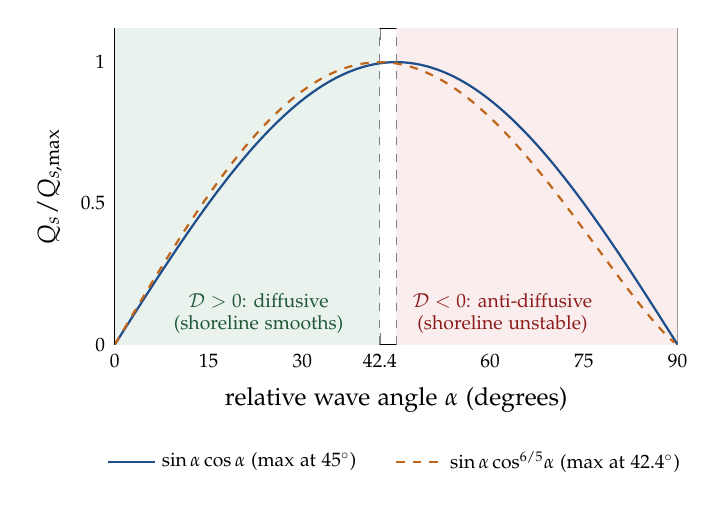
\begin{tikzpicture}
\begin{axis}[width=0.72\linewidth,height=5.6cm,xmin=0,xmax=90,ymin=0,ymax=1.12,
  xlabel={relative wave angle $\alpha$ (degrees)},ylabel={$Q_s/Q_{s,\max}$},
  xtick={0,15,30,42.4,60,75,90},xticklabels={0,15,30,42.4,60,75,90},
  legend style={font=\scriptsize,draw=none,fill=none,at={(0.5,-0.3)},anchor=north,legend columns=2,
  /tikz/every even column/.append style={column sep=1.2em}},
  tick label style={font=\scriptsize},label style={font=\small}]
\fill[resgreen!10] (axis cs:0,0) rectangle (axis cs:42.4,1.12);
\fill[pitred!8] (axis cs:45,0) rectangle (axis cs:90,1.12);
\addplot[thick,keyblue,domain=0:90,samples=120] {sin(2*x)};
\addplot[thick,exorange,dashed,domain=0:89.5,samples=120] {sin(x)*cos(x)^1.2/0.46869};
\draw[gray,dashed] (axis cs:45,0) -- (axis cs:45,1.12);
\draw[gray,dashed] (axis cs:42.4,0) -- (axis cs:42.4,1.12);
\node[font=\scriptsize,resgreen!70!black,align=center] at (axis cs:23,0.11) {$\mathcal{D}>0$: diffusive\\(shoreline smooths)};
\node[font=\scriptsize,pitred!80!black,align=center] at (axis cs:62,0.11) {$\mathcal{D}<0$: anti-diffusive\\(shoreline unstable)};
\legend{$\sin\alpha\cos\alpha$ (max at $45^\circ$),$\sin\alpha\cos^{6/5}\!\alpha$ (max at $42.4^\circ$)}
\end{axis}
\end{tikzpicture}
\caption{Alongshore sediment flux versus the angle between wave crests and the shoreline, for the classical angular dependence and
for the refraction-corrected law of \citet{ashton2006}. The shoreline diffusivity \eqref{eq:shorediff} is proportional to the slope of
these curves and changes sign at the flux maximum.}
\label{fig:shoreline}
\end{figure}

\subsection{Linear stability and the Fourier view}
Linearise about a straight shoreline, so that $\mathcal D\approx\mathcal D_0=D_{\mathrm{sf}}^{-1}\,dQ_s/d\alpha\,|_{\alpha_0}$. Normal modes
$y_s=\epsilon\,e^{ikx+\sigma t}$ then grow or decay at the rate
\begin{equation}\label{eq:growth}
\sigma=-\mathcal D_0k^2 .
\end{equation}
If $\mathcal D_0>0$ every mode decays and the coast smooths, exactly like a degrading fault scarp (Section~\ref{sec:B2}). If
$\mathcal D_0<0$ every mode grows, and the shortest ones fastest: this is the backward heat equation, which is ill-posed as a
continuum model. The delta function makes the point vividly. A localised initial bump $y_s(x,0)=A\,\delta(x)$ contains all wavenumbers
in equal amounts (Section~\ref{sec:B4}); for $\mathcal D_0>0$ it relaxes into the Gaussian $A\,G(x,t)$ of \eqref{eq:heatkernel}, whereas for
$\mathcal D_0<0$ its shortest scales explode.

\begin{research}[emergent coastline shapes]
Real coasts do not blow up at the grid scale. At finite amplitude, protruding features shadow parts of the coast from the waves, and
the nonlinear angular dependence limits growth; large-scale cuspate capes, flying spits and alongshore sand waves then
self-organise \citep{ashton2001,ashton2006}. The deep lesson for complex Earth-surface systems is that a few robust, simplified
rules --- here, sediment conservation plus a flux law with a maximum --- can explain emergent patterns that detailed models struggle
to reproduce, which is the case for reduced-complexity models \citep{murray2007,murray2009}. Related instabilities underlie braided
rivers \citep{murray1994}, dune fields \citep{werner1995}, channelisation of hillslopes \citep{smith1972} and meandering
\citep{ikeda1981}.
\end{research}

\subsection{A more realistic flux law}
Including wave refraction and shoaling over shore-parallel contours, \citet{ashton2006} expressed the flux in terms of deep-water wave
height $H_0$, period $T$ and angle $\alpha$ as
\[
Q_s\propto H_0^{12/5}\,T^{1/5}\cos^{6/5}\!\alpha\,\sin\alpha
\qquad\Longrightarrow\qquad
\od{Q_s}{\alpha}\propto\cos^{1/5}\!\alpha\,\Big(\cos^2\alpha-\tfrac65\sin^2\alpha\Big),
\]
which changes sign at $\tan\alpha=\sqrt{5/6}$, i.e.\ at $\alpha_c\approx42.4^\circ$ (Exercise~\ref{ex:threshold}).

\begin{pycode}[where the shoreline diffusivity changes sign]
import sympy as sp
a = sp.symbols('alpha', positive=True)     # wave angle rel. to shoreline
laws = {"sin*cos": sp.sin(a)*sp.cos(a),
        "sin*cos^(6/5)": sp.sin(a)*sp.cos(a)**sp.Rational(6, 5)}
for name, Q in laws.items():
    crit = sp.nsolve(sp.diff(Q, a), a, 0.7)    # D ~ dQ/dalpha = 0
    print(f"{name:14s}: D changes sign at {float(sp.deg(crit)):.2f} deg")
# -> sin*cos       : D changes sign at 45.00 deg
# -> sin*cos^(6/5) : D changes sign at 42.39 deg
\end{pycode}

\subsection*{Exercises for Section~\ref{sec:capstone}}

\begin{exercise}[Deriving the shoreline diffusion equation]{2}{shorediff}
(a) Derive \eqref{eq:shorediff} from \eqref{eq:oneline}, including the factor $[1+(\partial y_s/\partial x)^2]^{-1}$.
(b) Which assumption of the one-line model corresponds to a ``kinematic'' treatment in the sense of Section~\ref{sec:B1}?
\end{exercise}

\begin{exercise}[Growth rates and length scales]{2}{growthrates}
(a) Derive \eqref{eq:growth}.
(b) For an illustrative $|\mathcal D_0|=0.05\units{km^2\,yr^{-1}}$ in the unstable regime, compute the $e$-folding times of perturbations with
wavelengths $5\units{km}$ and $1\units{km}$.
(c) Why does a model based on \eqref{eq:shorediff} alone need an additional physical ingredient (or a numerical regularisation) to
produce features of a preferred size?
\end{exercise}

\begin{exercise}[The 42-degree threshold]{2}{threshold}
Show that $d(\sin\alpha\cos^{6/5}\!\alpha)/d\alpha=\cos^{1/5}\!\alpha\,(\cos^2\alpha-\tfrac65\sin^2\alpha)$ and that it vanishes at
$\alpha_c=\arctan\sqrt{5/6}\approx42.4^\circ$.
\end{exercise}

\begin{exercise}[Your own system]{3}{ownsystem}
Choose an Earth-surface system from your own research. (a) What is conserved, and what is its flux? (b) On which local gradient or
orientation does the flux depend? (c) Use the chain rule, as in \eqref{eq:shorediff}, to write an effective diffusivity or wave speed.
Can it change sign? (d) If it can, what physics limits growth at small scales and selects a pattern size?
\end{exercise}

% =====================================================================
\clearpage
\appendix
\section{Formula Sheet}\label{app:formulas}
% =====================================================================
\setlength{\columnsep}{18pt}
\begin{multicols}{2}
\small\raggedright
\newcommand{\fsh}[1]{\par\smallskip\noindent{\bfseries\color{keyblue}#1}\par\nopagebreak}
\newenvironment{fsl}{\begin{itemize}[leftmargin=0.9em,itemsep=1.5pt,topsep=1pt,label={\textcolor{srcpurple}{\scriptsize$\blacktriangleright$}}]}{\end{itemize}}

\fsh{B.1 Derivatives and characteristics}
\begin{fsl}
  \item $Df/Dt=\partial_tf+\uu\cdot\nabla f=\partial_tf+u_i\,\partial_if$
  \item along a path $\XX(t)$: $df/dt=\partial_tf+(dX_i/dt)\,\partial_if$
  \item $Af_t+Bf_x=g$: \ $dt/ds=A$, $dx/ds=B$, $df/ds=g$
  \item Example B.1: $f=\phi\big(x-\int_0^tU\,d\tau\big)$
  \item kinematic wave: $a_t+q_x=0$, $q(a)\Rightarrow c=dq/da$; shock speed $V=[q]/[a]$
  \item Leibniz: $\frac{d}{dx}\int_a^bf\,dz=\int_a^bf_x\,dz+f(b)\,b'-f(a)\,a'$
  \item kinematic BC at $z=\zeta$: $w=\zeta_t+u\zeta_x+v\zeta_y$
  \item depth-averaged continuity: $h_t+\nabla_h\cdot(h\bar\uu)=0$
\end{fsl}

\fsh{B.2 Changing variables}
\begin{fsl}
  \item $\partial/\partial(\text{old})=\sum\big(\partial\,\text{new}/\partial\,\text{old}\big)\,\partial/\partial(\text{new})$; say what is held fixed
  \item moving frame $\xi=x-Ut$, $\tau=t$: \ $\partial_x=\partial_\xi$, \ $\partial_t=\partial_\tau-U\partial_\xi$
  \item frozen pattern $f=F(x-ct)$: \ $f_t=-c\,f_x$
  \item $\eta=xt^\alpha$: $f_x=t^\alpha f'$, $f_t=(\alpha/t)\,\eta f'$, $f_{xx}=t^{2\alpha}f''$
  \item diffusion, step $\pm a$: $f=a\erf\big(x/\sqrt{4\kappa t}\big)$; scarp $S_{\max}=a/\sqrt{\pi\kappa t}+b$
  \item $\chi=\int_0^x(A_0/A)^{m/n}dx'$; steady $z=z_{\mathrm{base}}+(\Up/KA_0^m)^{1/n}\chi$
  \item dune tracking: $q_s=(1-\lambda_p)\,c\,z_b+q_0$, \ $\bar q_s\approx\frac12(1-\lambda_p)\,cH$
\end{fsl}

\fsh{B.3 Vector calculus}
\begin{fsl}
  \item $(\nabla\times\uu)_i=\varepsilon_{ijk}\partial_ju_k$; \ $\varepsilon_{ijk}\varepsilon_{ilm}=\delta_{jl}\delta_{km}-\delta_{jm}\delta_{kl}$
  \item $\nabla\times\nabla\rho=0$, \ $\nabla\cdot(\nabla\times\uu)=0$, \ $\nabla\times\nabla\times\uu=\nabla(\nabla\cdot\uu)-\nabla^2\uu$
  \item $\nabla\cdot(\rho\uu)=\rho\nabla\cdot\uu+\uu\cdot\nabla\rho$; \ $\nabla\times(\rho\uu)=\rho\nabla\times\uu+\nabla\rho\times\uu$
  \item Lamb form: $(\uu\cdot\nabla)\uu=\nabla\big(\frac12|\uu|^2\big)-\uu\times\bomega$
  \item Gauss: $\int_A\uu\cdot\nn\,dA=\int_V\nabla\cdot\uu\,dV$, \ $\int_A\rho\,\nn\,dA=\int_V\nabla\rho\,dV$
  \item Stokes: $\oint_C\uu\cdot\tv\,ds=\int_A(\nabla\times\uu)\cdot\nn\,dA$
  \item budget $\Rightarrow$ PDE: $\partial_t(\cdot)+\nabla\cdot(\text{flux})=\text{sources}$
  \item Exner: $(1-\lambda_p)\,\partial_tz_b=-\nabla_h\cdot\qq_s$; \ hillslope: $\partial_tz=\Up+\kappa\nabla^2z$
  \item Darcy: $\qq=-K_h\nabla h$, \ $\nabla\cdot(K_h\nabla h)=0$
\end{fsl}

\fsh{B.4 Dirac delta}
\begin{fsl}
  \item $\int f(x)\,\delta(x-x_0)\,dx=f(x_0)$; \ $\delta_\sigma=e^{-x^2/2\sigma^2}/(\sqrt{2\pi}\,\sigma)$
  \item $x\,\delta(x-a)=a\,\delta(x-a)$; \ $\delta(\alpha x)=\delta(x)/|\alpha|$
  \item $\delta(g(x))=\sum_n\delta(x-x_n)/|g'(x_n)|$; \ $\int f\,\delta'(x-x_0)\,dx=-f'(x_0)$
  \item $H'=\delta$; \ units $[\delta(x)]=[x]^{-1}$
  \item cylindrical: $\delta(\xx-\xx_0)=\delta(R-R_0)\,\delta(\varphi-\varphi_0)\,\delta(z-z_0)/R_0$
  \item spherical: $\delta(\xx-\xx_0)=\delta(r-r_0)\,\delta(\theta-\theta_0)\,\delta(\varphi-\varphi_0)/(r_0^2\sin\theta_0)$
  \item diffusion kernel $G=(4\pi\kappa t)^{-1/2}e^{-x^2/4\kappa t}$, variance $2\kappa t$
  \item superposition $f=\iint G\,s\,d\xi\,d\tau$; \ $\nabla\cdot(\xx/|\xx|^3)=4\pi\delta(\xx)$
\end{fsl}

\fsh{B.5 Coordinate systems}
\begin{fsl}
  \item $h_i=|\partial\xx/\partial q_i|$, \ $\e{i}=h_i^{-1}\,\partial\xx/\partial q_i$
  \item $dV=h_1h_2h_3\,dq_1dq_2dq_3$; \ $\nabla=\sum_i\e{i}\,h_i^{-1}\partial/\partial q_i$
  \item cylindrical $(R,\varphi,z)$: $h=(1,R,1)$; \ $\partial_\varphi\e{R}=\e{\varphi}$, $\partial_\varphi\e{\varphi}=-\e{R}$
  \item spherical $(r,\theta,\varphi)$: $h=(1,r,r\sin\theta)$
  \item $\partial_\theta\e{r}=\e{\theta}$, \ $\partial_\varphi\e{r}=\sin\theta\,\e{\varphi}$, \ $\partial_\theta\e{\theta}=-\e{r}$
  \item $\partial_\varphi\e{\theta}=\cos\theta\,\e{\varphi}$, \ $\partial_\varphi\e{\varphi}=-\sin\theta\,\e{r}-\cos\theta\,\e{\theta}$
  \item sphere: $dA=a^2\sin\theta\,d\theta\,d\varphi$; \ lat--lon cell $R_E^2\,\Delta\lambda\,(\sin\vartheta_2-\sin\vartheta_1)$
  \item cylindrical acceleration: $Du_R/Dt-u_\varphi^2/R$, \ $Du_\varphi/Dt+u_Ru_\varphi/R$, \ $Du_z/Dt$
\end{fsl}

\fsh{B.6 Curvilinear equations}
\begin{fsl}
  \item $\nabla\cdot\uu=H^{-1}\sum_i\partial_i(Hu_i/h_i)$, \ $\nabla^2f=H^{-1}\sum_i\partial_i(Hh_i^{-2}\,\partial_if)$, \ $H=h_1h_2h_3$
  \item $\nabla^2\uu=\nabla(\nabla\cdot\uu)-\nabla\times(\nabla\times\uu)$ \ (never component-wise)
  \item cyl.: $(\nabla^2\uu)_R=\nabla^2u_R-u_R/R^2-(2/R^2)\,\partial_\varphi u_\varphi$
  \item cyl.: $(\nabla^2\uu)_\varphi=\nabla^2u_\varphi+(2/R^2)\,\partial_\varphi u_R-u_\varphi/R^2$
  \item sph.\ extra acceleration terms: $r$: $-(u_\theta^2+u_\varphi^2)/r$; \ $\theta$: $u_ru_\theta/r-u_\varphi^2\cot\theta/r$; \
        $\varphi$: $u_\varphi u_r/r+u_\theta u_\varphi\cot\theta/r$
  \item $S_{R\varphi}=\frac R2\,\partial_R(u_\varphi/R)+\frac{1}{2R}\,\partial_\varphi u_R$ \ (zero for rigid rotation)
  \item vortices: $\omega_z=R^{-1}d(Ru_\varphi)/dR$; point vortex $\omega_z=\Gamma\,\delta(x)\,\delta(y)$
  \item Poiseuille: $u_z=G(a^2-R^2)/(4\mu)$, \ $Q=\pi Ga^4/(8\mu)$
  \item Stokes: $F_D=6\pi\mu aU$; \ $w_s=R_sgd^2/(18\nu)$ \ ($Re_p\lesssim1$)
  \item bend: $\partial\zeta/\partial R\approx u_\varphi^2/(gR)$
  \item wells: $h=h_w+\frac{Q}{2\pi T}\ln\frac{r}{r_w}$ (Thiem), \ $s=\frac{Q}{4\pi T}E_1\!\big(\frac{r^2S}{4Tt}\big)$ (Theis)
\end{fsl}
\end{multicols}

% =====================================================================
\section{Answers to the Warm-up Diagnostic}\label{app:quiz}
% =====================================================================
\begin{enumerate}[label=\textbf{Q\arabic*.},leftmargin=2.4em]
  \item Not necessarily. A constant reading means $\partial T/\partial t=0$, but $DT/Dt=u\,\partial T/\partial x$ need not vanish: each parcel can warm
        while cooler parcels keep arriving from upstream (\S\ref{sec:B1}).
  \item $f=\exp[-(x-3t)^2]$: the profile translates at speed 3 along the characteristics $x-3t=\text{const}$.
  \item $(\partial/\partial t)_x=\partial/\partial\tau-U\,\partial/\partial\xi$ and $(\partial/\partial x)_t=\partial/\partial\xi$ (Example B.2).
  \item $\eta=x/\sqrt{4Dt}$ (any multiple of $x/\sqrt t$); the solution is an error function.
  \item Both vanish for smooth fields. Hence vorticity is solenoidal (vortex lines cannot end in the fluid) and gradient fields are
        irrotational (potential flow, Darcy flow).
  \item $\int_V\nabla\cdot\qq\,dV=\int_A\qq\cdot\nn\,dA$. Shrinking $V$ to a point gives $\nabla\cdot\qq=\lim V^{-1}\int_A\qq\cdot\nn\,dA$: the outward flux per
        unit volume.
  \item $e^2$ and $1/3$; $\delta(x)$ has units of $\mathrm{m^{-1}}$.
  \item $dA=a^2\sin\theta\,d\theta\,d\varphi$. The direction of $\e{R}$ depends on $\varphi$ (it rotates with the azimuth): $\partial\e{R}/\partial\varphi=\e{\varphi}$.
  \item It is the centripetal acceleration that arises because $\e{\varphi}$ changes direction along a particle path; it is geometry, not a new force.
  \item No, except on the axis: $\omega_z=R^{-1}d(Ru_\varphi)/dR=0$ for $R\neq0$. All the vorticity is concentrated at $R=0$,
        $\omega_z=\Gamma\,\delta(x)\,\delta(y)$ (\S\ref{sec:B6}).
\end{enumerate}

\clearpage
% =====================================================================
\section{Solutions to the Exercises}\label{app:solutions}
% =====================================================================
\ifshowsolutions
Try each exercise before reading its solution. Numbers are rounded to two or three significant figures.

\subsection*{Section~\ref{sec:B1}: Partial and total differentiation}

\begin{solution}{threederiv}
(a) $\partial f/\partial t=-x^2y\,e^{-t}$ and $\partial f/\partial x=2xy\,e^{-t}$. Both mixed derivatives equal $-2xy\,e^{-t}$.

(b) With $\dot X=1$ and $\dot Y=2t$,
$df/dt=-x^2ye^{-t}+2xye^{-t}\cdot1+x^2e^{-t}\cdot2t$, which at $x=t$, $y=1+t^2$ becomes $e^{-t}(2t-t^2+4t^3-t^4)$.
Directly, $f(t)=(t^2+t^4)e^{-t}$, so $df/dt=(2t+4t^3)e^{-t}-(t^2+t^4)e^{-t}$: the same.

(c) $Df/Dt=\partial_tf+u\,\partial_xf+v\,\partial_yf=-x^2ye^{-t}+(-y)(2xye^{-t})+x(x^2e^{-t})=e^{-t}(x^3-x^2y-2xy^2)$.
\end{solution}

\begin{solution}{stretch}
The characteristics obey $dX/dt=aX$, so $X=X_0e^{at}$, and $f$ is constant along them: $f(x,t)=\phi(xe^{-at})$. For
$\phi=\exp(-x^2/\ell^2)$, $f=\exp[-x^2/(\ell e^{at})^2]$: the patch keeps its peak value but its width grows as $\ell e^{at}$. For $a<0$ the flow
converges, the patch narrows as $\ell e^{-|a|t}$ and its gradients sharpen (the pitfall in Section~\ref{sec:B1}). Note that $f$ behaves like an
intensive property (e.g.\ temperature); a conserved \emph{density} would obey $\partial_tc+\partial_x(acx)=0$ instead, and its peak would decrease as
$e^{-at}$ while the patch spreads.
\end{solution}

\begin{solution}{settling}
(a) All characteristics are lines of slope $dx/dt=U$, and along each $dC/dt=-(w_s/h)C$. Those starting on the initial line ($x=X_0>0$ at $t=0$)
carry $C=0$ and fill the region $x>Ut$, so $C=0$ there. Those starting on the boundary ($x=0$ at $t=T_0>0$) carry $C_{\mathrm{in}}$, and fill
$x<Ut$. A parcel that entered at $T_0=t-x/U$ has been settling for a time $x/U$, so
\[
C(x,t)=C_{\mathrm{in}}\exp\!\left(-\frac{w_s}{h}\frac{x}{U}\right)=C_{\mathrm{in}}e^{-x/L_s}\quad(x<Ut),\qquad C=0\quad(x>Ut).
\]
(b) Behind the front, $C$ does not depend on $t$: the profile is steady and decays over $L_s=Uh/w_s=(1)(2)/(10^{-3})=2000\units{m}$. Coarse silt
travels kilometres before settling, whereas fine sand ($w_s\approx2\units{cm\,s^{-1}}$) settles within about a hundred metres. The front stays sharp only because diffusion
has been neglected.
\end{solution}

\begin{solution}{knick}
(a) With $m=\tfrac12$, $dx_k/dt=KA^{1/2}=K\sqrt{k_a}\,(L-x_k)$. Writing $\ell=L-x_k$ (distance from the divide), $d\ell/dt=-\beta\ell$ with
$\ell(0)=L$, so $\ell=Le^{-\beta t}$.
(b) $t=\beta^{-1}\ln(L/\ell)=\ln(20)/(2\times10^{-6}\units{yr^{-1}})\approx1.50\times10^{6}\units{yr}$, in agreement with the Python check.
(c) No: $\ell\to0$ only as $t\to\infty$ because the celerity vanishes at the divide. Near channel heads drainage area is small and the stream-power
law ceases to apply; hillslope diffusion, landsliding and debris flows take over and communicate the base-level signal to the ridges.
\end{solution}

\begin{solution}{flood}
(a) Ch\'ezy: $q=C_zS_0^{1/2}h^{3/2}$, so $c=dq/dh=\tfrac32C_zS_0^{1/2}h^{1/2}=\tfrac32U$. Manning: $q=n_M^{-1}S_0^{1/2}h^{5/3}$, so $c=\tfrac53U$.
(b) $c=3.0\units{m\,s^{-1}}$ (Ch\'ezy) or $3.3\units{m\,s^{-1}}$ (Manning), faster than the water.
(c) Depth is constant along characteristics moving at $c(h)$, which increases with $h$. On the rising limb the deeper water behind travels
faster than the shallower water ahead, so the limb is compressed and steepens; the falling limb is stretched.
(d) Mass conservation across the jump gives $V=(q_2-q_1)/(h_2-h_1)=C_zS_0^{1/2}\,(h_2^{3/2}-h_1^{3/2})/(h_2-h_1)$, which lies between $c(h_1)$ and
$c(h_2)$ and tends to $c$ as $h_1\to h_2$.
\end{solution}

\begin{solution}{integrate}
(a) $\partial_x(\partial_yf)=0$ means $\partial_yf=g(y)$, so $f=F(x)+G(y)$ with arbitrary $F$ and $G$.
(b) $f=x^2y+x+g(y)$ from the first equation; the second then requires $g'(y)=\cos y$, so $f=x^2y+x+\sin y+C$. (Check:
$\partial_y(2xy+1)=2x=\partial_x(x^2+\cos y)$.)
(c) $\partial_y(-y)=-1\neq\partial_x(x)=1$, so no such $f$ exists. $(-y,x)$ is solid-body rotation with $\omega_z=2$: a rotational field cannot be the gradient
of a potential, consistent with (B.3.11).
\end{solution}

\begin{solution}{leibniz}
By Leibniz' rule, $\int_{z_b}^{\zeta}\partial_xu\,dz=\partial_x\!\int_{z_b}^{\zeta}u\,dz-u_\zeta\,\partial_x\zeta+u_b\,\partial_xz_b$, and
$\int_{z_b}^{\zeta}\partial_zw\,dz=w_\zeta-w_b$, where subscripts $\zeta$ and $b$ denote surface and bed values. Adding,
\[
\partial_x(h\bar u)-u_\zeta\partial_x\zeta+u_b\partial_xz_b+w_\zeta-w_b=0 .
\]
The kinematic conditions $w_\zeta=\partial_t\zeta+u_\zeta\partial_x\zeta$ and $w_b=u_b\,dz_b/dx$ cancel four terms, leaving
$\partial_t\zeta+\partial_x(h\bar u)=0$. Because the bed is fixed, $\partial_t\zeta=\partial_th$.
\end{solution}

\begin{solution}{cosmo}
(a) Following a parcel, $dN/dt=P_0e^{-Z/z_*}-\lambda N$ with $dZ/dt=-\varepsilon$. For $N(Z,t)$ in the surface frame, the chain rule gives
$dN/dt=\partial_tN+(dZ/dt)\,\partial_Z N$, so
$\partial_tN-\varepsilon\,\partial_Z N=P_0e^{-Z/z_*}-\lambda N$: the ``material derivative'' is $\partial_t-\varepsilon\partial_Z$.

(b) At steady state, $-\varepsilon N'+\lambda N=P_0e^{-Z/z_*}$. Trying $N=Be^{-Z/z_*}$ gives $B(\varepsilon/z_*+\lambda)=P_0$. The homogeneous
solution $\propto e^{\lambda Z/\varepsilon}$ grows with depth and is excluded. Hence $N=P_0e^{-Z/z_*}/(\lambda+\varepsilon/z_*)$ and
$N_0=P_0/(\lambda+\varepsilon/z_*)$.

(c) $\varepsilon=z_*(P_0/N_0-\lambda)$. With $\lambda=\ln2/1.387\units{Myr}=5.0\times10^{-7}\units{yr^{-1}}$, $z_*=60.4\units{cm}$ and
$P_0/N_0=4.0\times10^{-5}\units{yr^{-1}}$: $\varepsilon=60.4\times3.95\times10^{-5}\approx2.4\times10^{-3}\units{cm\,yr^{-1}}\approx24\units{m\,Myr^{-1}}$.
The concentration averages erosion over $z_*/\varepsilon\approx25\units{kyr}$.
\end{solution}

\subsection*{Section~\ref{sec:B2}: Changing independent variables}

\begin{solution}{galilean}
(a) By \eqref{eq:B22}, $\partial_tf=\partial_\tau F-U\partial_\xi F$, $\partial_xf=\partial_\xi F$ and $\partial_x^2f=\partial_\xi^2F$. Substituting,
$\partial_\tau F-U\partial_\xi F+U\partial_\xi F=\kappa\,\partial_\xi^2F$: the advection terms cancel.
(b) $f(x,t)=M(4\pi\kappa t)^{-1/2}\exp[-(x-Ut)^2/(4\kappa t)]$: a Gaussian whose centre moves at $U$ and whose variance grows as $2\kappa t$.
\end{solution}

\begin{solution}{heldconstant}
With $s=x-Ut$: $(\partial f/\partial t)_x=(2Us/L^2)f$, $(\partial f/\partial x)_t=-(2s/L^2)f$, and for $F=\exp(-\xi^2/L^2)$:
$(\partial F/\partial\tau)_\xi=0$, $(\partial F/\partial\xi)_\tau=-(2\xi/L^2)F$. Then $\partial_\tau F-U\partial_\xi F=2U\xi F/L^2=(\partial f/\partial t)_x$, as \eqref{eq:B22} requires.
A fixed observer sees the pulse rise and fall as it passes; an observer riding with it sees no change.
\end{solution}

\begin{solution}{polarlap}
Write $c=\cos\theta$ and $s=\sin\theta$. Applying $\partial_x=c\,\partial_r-(s/r)\partial_\theta$ to $\partial_x\psi=c\psi_r-(s/r)\psi_\theta$, and remembering that the
operators also act on $c$ and $s/r$,
\[
\psi_{xx}=c^2\psi_{rr}-\frac{2sc}{r}\psi_{r\theta}+\frac{s^2}{r}\psi_r+\frac{2sc}{r^2}\psi_\theta+\frac{s^2}{r^2}\psi_{\theta\theta},\qquad
\psi_{yy}=s^2\psi_{rr}+\frac{2sc}{r}\psi_{r\theta}+\frac{c^2}{r}\psi_r-\frac{2sc}{r^2}\psi_\theta+\frac{c^2}{r^2}\psi_{\theta\theta}.
\]
Adding, the mixed and $\psi_\theta$ terms cancel: $\nabla^2\psi=\psi_{rr}+r^{-1}\psi_r+r^{-2}\psi_{\theta\theta}=r^{-1}\partial_r(r\psi_r)+r^{-2}\psi_{\theta\theta}$.
\end{solution}

\begin{solution}{scarp}
(a) The equation is linear, $bx$ is a steady solution, and $a\erf(\eta)$ solves it (Worked example~\ref{we:erf}). As $t\to0^+$,
$\erf(x/\sqrt{4\kappa t})\to\sgn(x)$.
(b) $\kappa t=a^2/[\pi(S_{\max}-b)^2]=4/(\pi\times0.25^2)=20.4\units{m^2}$; with $\kappa=1\units{m^2\,kyr^{-1}}$ the scarp is about $20\units{kyr}$ old.
(c) $S_{\max}-b\propto(\kappa t)^{-1/2}$, so halving it requires $\kappa t$ to grow fourfold.
(d) $\partial_xz-b=a\,(2/\sqrt\pi)\,e^{-\eta^2}/\sqrt{4\kappa t}=2a\,e^{-x^2/4\kappa t}/\sqrt{4\pi\kappa t}=2aG$. Differentiating the diffusion equation with respect
to $x$ shows that the slope also diffuses; its initial condition is $2a\,\delta(x)+b$, and the response to a delta is $G$ (Section~\ref{sec:B4}).
\end{solution}

\begin{solution}{dunes}
$\bar q_s=\beta(1-\lambda_p)cH=0.5\times0.65\times(1.5/3600\units{m\,s^{-1}})\times0.8\units{m}=1.1\times10^{-4}\units{m^2\,s^{-1}}$ of grains, or
$\rho_s\bar q_s\approx0.29\units{kg\,m^{-1}\,s^{-1}}$. Across a $100\units{m}$ wide channel that is about $29\units{kg\,s^{-1}}$, or $2500$ tonnes per day.
\end{solution}

\begin{solution}{chi}
(a) For $n=1$, $d\chi/dx=(A_0/A)^m$, so
\begin{gather*}
\partial_xz=(A_0/A)^m\,\partial_\chi z,\qquad KA^m\partial_xz=KA_0^m\,\partial_\chi z,\\
\text{hence}\quad \partial_tz+KA_0^m\,\partial_\chi z=\Up .
\end{gather*}
(b) At steady state $KA^mS^n=\Up$, i.e.
\[
\od{z}{x}=\left(\frac{\Up}{KA^m}\right)^{1/n}=\left(\frac{\Up}{KA_0^m}\right)^{1/n}\left(\frac{A_0}{A}\right)^{m/n}=\left(\frac{\Up}{KA_0^m}\right)^{1/n}\od{\chi}{x}.
\]
Integrating from base level gives $z=z_{\mathrm{base}}+(\Up/KA_0^m)^{1/n}\chi$.
(c) With uniform $K$, in $\chi$-space the knickpoint moves at the constant speed $KA_0^m$ on every flow path, starting from $\chi=0$
at base level; once it has passed the junction it continues independently up each tributary. After $1\units{Myr}$ it is at
$\chi_k=KA_0^m\times10^6\units{yr}$ in both tributaries, although their distances from the junction differ.
\end{solution}

\begin{solution}{gravcurrent}
(a) With $h=t^\beta F(\eta)$ and $\eta=x/t^\alpha$: $\partial_th=t^{\beta-1}(\beta F-\alpha\eta F')$ and
$\gamma\partial_x(h^3\partial_xh)=\gamma t^{4\beta-2\alpha}(F^3F')'$. Time cancels if $\beta-1=4\beta-2\alpha$, i.e.\ $2\alpha-3\beta=1$.
(b) $\int h\,dx=t^{\alpha+\beta}\int F\,d\eta$. Fixed volume: $\beta=-\alpha$, so $5\alpha=1$ and $\alpha=\tfrac15$. Constant supply: $\alpha+\beta=1$, so
$2\alpha-3(1-\alpha)=1$ and $\alpha=\tfrac45$.
(c) The axisymmetric operator has the same scaling, so again $2\alpha-3\beta=1$, while the volume $2\pi\int hR\,dR\propto t^{\beta+2\alpha}$ must scale as
$t^p$: $\beta=p-2\alpha$ and $\alpha=(1+3p)/8$, i.e.\ $t^{1/8}$ for a fixed volume and $t^{1/2}$ for a constant flux, as found by \citet{huppert1982}.
\end{solution}

\subsection*{Section~\ref{sec:B3}: Vector calculus}

\begin{solution}{fourflows}
(i) $\nabla\cdot\uu=0$, $\omega_z=0$: parallel streamlines. (ii) $\nabla\cdot\uu=\alpha-\alpha=0$, $\omega_z=0$: hyperbolic streamlines $xy=\text{const}$
(stagnation-point flow). (iii) $\nabla\cdot\uu=0$, $\omega_z=2\Omega$: circles. (iv) $\nabla\cdot\uu=0$, $\omega_z=-\gamma$: straight streamlines. Flows (iii) and
(iv) are rotational. In simple shear a small cross of fluid lines rotates on average: the line along $y$ is tilted by the shear while the line along
$x$ is not, so the mean angular velocity is $-\gamma/2$ --- vorticity measures the rotation of fluid elements, not the curvature of their paths.
\end{solution}

\begin{solution}{productrules}
(a) $\partial_i(\rho u_i)=\rho\,\partial_iu_i+u_i\partial_i\rho$, which is (B.3.6). $[\nabla\times(\rho\uu)]_i=\varepsilon_{ijk}\partial_j(\rho u_k)=\rho\,\varepsilon_{ijk}\partial_ju_k+\varepsilon_{ijk}(\partial_j\rho)u_k$,
which is (B.3.7).
(b) $\partial_t\rho+\nabla\cdot(\rho\uu)=\partial_t\rho+\uu\cdot\nabla\rho+\rho\nabla\cdot\uu=D\rho/Dt+\rho\nabla\cdot\uu$. The conservative form is a mass budget for a fixed
volume (flux divergence); the advective form says that a parcel's density changes only by expansion or compression. Incompressible flow means
$D\rho/Dt=0$, equivalently $\nabla\cdot\uu=0$.
\end{solution}

\begin{solution}{stretching}
(a) $[\nabla\times(\uu\times\FF)]_i=\varepsilon_{kij}\varepsilon_{klm}\partial_j(u_lF_m)=(\delta_{il}\delta_{jm}-\delta_{im}\delta_{jl})(F_m\partial_ju_l+u_l\partial_jF_m)
=F_j\partial_ju_i+u_i\partial_jF_j-F_i\partial_ju_j-u_j\partial_jF_i$, which is (B.3.10).
(b) With $\FF=\bomega$, $\nabla\cdot\uu=0$ and $\nabla\cdot\bomega=0$ (B.3.12), two terms vanish.
(c) With \eqref{eq:lamb}, $\partial_t\uu+\nabla(\tfrac12|\uu|^2)-\uu\times\bomega=-\nabla p/\rho+\nu\nabla^2\uu$. The curl removes the gradients:
$\partial_t\bomega-\nabla\times(\uu\times\bomega)=\nu\nabla^2\bomega$, and (b) gives $D\bomega/Dt=(\bomega\cdot\nabla)\uu+\nu\nabla^2\bomega$.
\end{solution}

\begin{solution}{bernoulli}
(a) With $\FF=\uu$ in (B.3.9): $\nabla(|\uu|^2)=2\uu\times\bomega+2(\uu\cdot\nabla)\uu$.
(b) Substituting \eqref{eq:lamb}: $\nabla(\tfrac12|\uu|^2)-\uu\times\bomega=-\nabla(p/\rho)-\nabla(gz)$, i.e.\ $\nabla B=\uu\times\bomega$. Since $\uu\cdot(\uu\times\bomega)=0$,
$\uu\cdot\nabla B=0$: $B$ is constant along streamlines, and everywhere if $\bomega=0$.
(c) Hydrostatic pressure gives $p/\rho+gz=g(z_b+h)$ throughout the depth, so $B/g=z_b+h+U^2/(2g)=z_b+E$. Constancy of $B$ over a frictionless bed is the
statement $E+z_b=\text{const}$ used for flow over bumps and through contractions.
\end{solution}

\begin{solution}{ridge}
(a) $\kappa z''=-\Up$ with $z'(0)=0$ gives $z=z_c-\Up x^2/(2\kappa)$; the relief is $z_c-z(L_H)=\Up L_H^2/(2\kappa)$.
(b) Relief $=10^{-4}\times2500/(2\times0.005)=25\units{m}$; hilltop curvature $z''=-\Up/\kappa=-0.02\units{m^{-1}}$.
\end{solution}

\begin{solution}{exnergauss}
(a) $\dfrac{d}{dt}\int_\Omega(1-\lambda_p)z_b\,dA=-\oint_{\partial\Omega}\qq_s\cdot\nn\,ds+\int_\Omega\sigma\,dA$; the 2D divergence theorem turns the boundary integral into
$\int_\Omega\nabla_h\cdot\qq_s\,dA$, and localisation gives the result.
(b) $\partial_xq_s=q_0/L>0$: the flux diverges, so the bed degrades at the rate $q_0/[(1-\lambda_p)L]$.
\end{solution}

\begin{solution}{darcy}
(a) $\nabla\cdot(K_h\nabla h)=K_h\nabla^2h+\nabla K_h\cdot\nabla h=0$ by the product rule (B.3.6).
(b) By (B.3.7) and (B.3.11), $\nabla\times\qq=-(K_h\nabla\times\nabla h+\nabla K_h\times\nabla h)=-\nabla K_h\times\nabla h$. It vanishes where $K_h$ is uniform or
$\nabla K_h\parallel\nabla h$ (conductivity varying only along the flow direction).
(c) Flow oblique to layering in interbedded sands and clays, around buried channel sands, or across fault zones and karst conduits.
\end{solution}

\begin{solution}{pointsource}
(a) On $r=a$, $\mathbf F\cdot\nn=(\xx/r^3)\cdot(\xx/r)=1/a^2$, and the area is $4\pi a^2$: the flux is $4\pi$.
(b) Let $S$ enclose the origin and let $S_\epsilon$ be a small sphere inside it. In the region between them $\nabla\cdot\mathbf F=0$, so by Gauss' theorem the fluxes
through $S$ and $S_\epsilon$ are equal: $4\pi$. A surface not enclosing the origin has zero flux. Hence $\int_V\nabla\cdot\mathbf F\,dV=4\pi$ if $V$ contains the origin and
$0$ otherwise, which is the definition of $4\pi\delta(\xx)$.
(c) $\nabla(1/r)=-\xx/r^3$, so $\nabla^2(1/r)=-4\pi\delta(\xx)$. For a source, $\nabla\cdot\qq=Q\delta(\xx)$ with $\qq=-K_h\nabla h$, so $\nabla^2h=-(Q/K_h)\delta(\xx)$,
solved by $h=h_\infty+Q/(4\pi K_hr)$.
\end{solution}

\subsection*{Section~\ref{sec:B4}: The Dirac delta}

\begin{solution}{deltaint}
(a) $1+2=3$. (b) $\cos2\pi=1$. (c) The spike at $x=-2$ is outside $[0,5]$: $0$. (d) $\delta(2x+4)=\tfrac12\delta(x+2)$, so $\tfrac12e^{-2}\approx0.068$.
(e) $-f'(a)$. (f) The roots of $x^2-4$ are $\pm2$ with $|g'|=4$, so $\delta(x^2-4)=\tfrac14[\delta(x-2)+\delta(x+2)]$ and the integral is $\tfrac12$.
\end{solution}

\begin{solution}{deltaprops}
(a) With $s=x/(\sqrt2\sigma)$, $\int\delta_\sigma\,dx=\pi^{-1/2}\int e^{-s^2}ds=1$. For fixed $x\neq0$, $e^{-x^2/2\sigma^2}$ decays faster than $1/\sigma$ grows.
(b) For $\alpha>0$, $s=\alpha x$ gives $\int f(s/\alpha)\,\delta(s)\,ds/\alpha=f(0)/\alpha$; for $\alpha<0$ the limits swap and the result is $f(0)/|\alpha|$.
(c) The left side has units $\mathrm{m\,s^{-1}}$ and $\delta(x-x_0)$ has units $\mathrm{m^{-1}}$, so $I$ has units $\mathrm{m^2\,s^{-1}}$. Integrating across $x_0$ shows
that $q_s$ jumps by $I$, so $I=Q_{\mathrm{in}}/B$.
\end{solution}

\begin{solution}{kernel}
(a) $G_t=G[-1/(2t)+x^2/(4\kappa t^2)]$ and $G_{xx}=G[-1/(2\kappa t)+x^2/(4\kappa^2t^2)]$, so $G_t=\kappa G_{xx}$. $G$ is a normal density with variance $2\kappa t$, so
its area is $1$ and $\int x^2G\,dx=2\kappa t$.
(b) $c=a\big[\int_0^\infty G(x-\xi)\,d\xi-\int_{-\infty}^0G(x-\xi)\,d\xi\big]=a\big[\tfrac12(1+\erf\eta)-\tfrac12(1-\erf\eta)\big]=a\erf\eta$, with $\eta=x/\sqrt{4\kappa t}$.
\end{solution}

\begin{solution}{tracer}
(a) $U=(2160-720)/1200=1.2\units{m\,s^{-1}}$ and $K_x=\Delta\sigma^2/(2\Delta t)=1200/2400=0.5\units{m^2\,s^{-1}}$. (Using differences removes the unknown initial
spreading: $\sigma^2=2K_xt$ would give $600\units{m^2}$ at $10\units{min}$, not $400$.)
(b) $c_{\max}=(M/A)/(\sqrt{2\pi}\,\sigma)=0.25/(\sqrt{2\pi}\times40)\approx2.5\times10^{-3}\units{kg\,m^{-3}}=2.5\units{mg\,L^{-1}}$ (or $2.35\units{mg\,L^{-1}}$ with
$\sigma^2=2K_xt$).
\end{solution}

\begin{solution}{hydrograph}
(a) $dV/dt+V/k=\delta(t)$ with $V(0^-)=0$: integrating across $t=0$ gives $V(0^+)=1$, and then $V=e^{-t/k}$, so $u=Q=k^{-1}e^{-t/k}H(t)$.
(b) $Q(t)=(P_1/k)\,e^{-t/k}H(t)+(P_2/k)\,e^{-(t-t_2)/k}H(t-t_2)$. $Q(0^+)=4.0\units{mm\,h^{-1}}$ and
$Q(t_2^+)=(20e^{-0.6}+10)/5=4.2\units{mm\,h^{-1}}$.
(c) Real catchments delay and smooth the response because water must travel through the network. A cascade of $n$ reservoirs gives
$u(t)=t^{n-1}e^{-t/k}/[k^n(n-1)!]$, which rises smoothly and peaks at $t=(n-1)k$ \citep{nash1957}.
\end{solution}

\begin{solution}{polardelta}
(a) $\iint f(r,\theta)\,\dfrac{\delta(r-r_0)\,\delta(\theta-\theta_0)}{r_0}\,r\,dr\,d\theta=f(r_0,\theta_0)\,\dfrac{r_0}{r_0}=f(r_0,\theta_0)$.
(b) The sink is $-(Q/b)\,\delta(x)\,\delta(y)$ per unit volume. On a cylinder of radius $R$ and height $b$ (impermeable top and bottom),
$\int\qq\cdot\nn\,dA=2\pi Rb\,q_R=\int_V\nabla\cdot\qq\,dV=-Q$, so $q_R=-Q/(2\pi bR)$.
\end{solution}

\begin{solution}{coarse}
(a) $\partial_t\delta_\sigma(x-x_p(t))=-v_p\,\delta_\sigma'(x-x_p)=-\partial_x[v_p\,\delta_\sigma(x-x_p)]$, since $v_p$ does not depend on $x$. Summing over $p$ gives the result.
(b) $J_\sigma/n_\sigma$ is the kernel-weighted mean velocity of grains near $x$. Choose $\sigma$ larger than the typical grain spacing (to suppress noise) but smaller
than the morphological scales to be resolved (bedforms, bars).
(c) Grains that start or stop moving add a source $E-D$ (entrainment minus deposition per unit length and time):
$\partial_tn+\partial_xJ=E-D$, the ``entrainment form'' of sediment conservation that complements the Exner equation for the bed \citep{furbish2012}.
\end{solution}

\subsection*{Section~\ref{sec:B5}: Coordinate systems}

\begin{solution}{cylunit}
$\partial_R\xx=(\cos\varphi,\sin\varphi,0)$, $\partial_\varphi\xx=R(-\sin\varphi,\cos\varphi,0)$, $\partial_z\xx=(0,0,1)$, so $(h_R,h_\varphi,h_z)=(1,R,1)$ and
$\e{R}=(\cos\varphi,\sin\varphi,0)$, $\e{\varphi}=(-\sin\varphi,\cos\varphi,0)$, $\e{z}=(0,0,1)$, which are mutually orthogonal unit vectors. Differentiating,
$\partial_\varphi\e{R}=(-\sin\varphi,\cos\varphi,0)=\e{\varphi}$ and $\partial_\varphi\e{\varphi}=(-\cos\varphi,-\sin\varphi,0)=-\e{R}$; all other derivatives vanish.
\end{solution}

\begin{solution}{sphunit}
$\partial_\varphi\e{r}=(-\sin\theta\sin\varphi,\sin\theta\cos\varphi,0)=\sin\theta\,\e{\varphi}$. Also $\partial_\varphi\e{\varphi}=(-\cos\varphi,-\sin\varphi,0)$, while
$-\sin\theta\,\e{r}-\cos\theta\,\e{\theta}=(-\cos\varphi,-\sin\varphi,-\sin\theta\cos\theta+\cos\theta\sin\theta)$, the same. Moving along a circle of latitude,
$\e{\varphi}$ turns about the $z$-axis, so its rate of change points horizontally toward the axis --- a direction with components along both $-\e{r}$
and $-\e{\theta}$.
\end{solution}

\begin{solution}{sphaccel}
$D\e{r}/Dt=\e{\theta}\,u_\theta/r+\sin\theta\,\e{\varphi}\,u_\varphi/(r\sin\theta)=(u_\theta\e{\theta}+u_\varphi\e{\varphi})/r$;
$D\e{\theta}/Dt=-\e{r}u_\theta/r+\e{\varphi}u_\varphi\cot\theta/r$; $D\e{\varphi}/Dt=-(\e{r}+\cot\theta\,\e{\theta})\,u_\varphi/r$. In
$D\uu/Dt=\sum_i(Du_i/Dt)\,\e{i}+\sum_iu_i\,D\e{i}/Dt$, the $\e{r}$ terms are $Du_r/Dt-u_\theta^2/r-u_\varphi^2/r$ and the $\e{\theta}$ terms are
$Du_\theta/Dt+u_ru_\theta/r-u_\varphi^2\cot\theta/r$.
\end{solution}

\begin{solution}{latlon}
(a) $A=\int_{\lambda_1}^{\lambda_2}\!\int_{\vartheta_1}^{\vartheta_2}R_E^2\cos\vartheta\,d\vartheta\,d\lambda=R_E^2\,\Delta\lambda\,(\sin\vartheta_2-\sin\vartheta_1)$.
(b) For small cells $A\approx R_E^2\,\Delta\lambda\,\Delta\vartheta\cos\vartheta$, which halves at $\vartheta=60^\circ$.
(c) Equal weights over-count the small high-latitude cells, biasing the mean toward high-latitude values; weight by $\cos\vartheta$ (or by exact cell areas).
\end{solution}

\begin{solution}{fan}
(a) $V=\int_0^\Theta\!\int_0^\infty T_0e^{-R/\ell_d}R\,dR\,d\varphi=\Theta T_0\ell_d^2$.
(b) $V=(\pi/2)\times5\times(2000)^2=3.1\times10^7\units{m^3}$.
(c) $\int_0^{\ell_d}Re^{-R/\ell_d}dR/\ell_d^2=1-2/e\approx0.26$: only a quarter of the volume lies within one decay length, because the area grows with $R$.
\end{solution}

\begin{solution}{caps}
(a) $A=\int_0^{2\pi}\!\int_{\vartheta_0}^{\pi/2}R_E^2\cos\vartheta\,d\vartheta\,d\lambda=2\pi R_E^2(1-\sin\vartheta_0)$.
(b) $(1-\sin60^\circ)/2=0.067$, i.e.\ $6.7\%$.
(c) The band $|\vartheta|<30^\circ$ has area $2\pi R_E^2[\sin30^\circ-\sin(-30^\circ)]=2\pi R_E^2$, half of $4\pi R_E^2$.
\end{solution}

\subsection*{Section~\ref{sec:B6}: Curvilinear equations}

\begin{solution}{mastercyl}
With $H=R$,
\[
\nabla\cdot\uu=\frac1R\big[\partial_R(Ru_R)+\partial_\varphi u_\varphi+\partial_z(Ru_z)\big],\qquad
\nabla^2\psi=\frac1R\big[\partial_R(R\psi_R)+\partial_\varphi(\psi_\varphi/R)+\partial_z(R\psi_z)\big],
\]
which reduce to the box. The $z$-component of the curl is
$(h_Rh_\varphi)^{-1}[\partial_R(h_\varphi u_\varphi)-\partial_\varphi(h_Ru_R)]=R^{-1}[\partial_R(Ru_\varphi)-\partial_\varphi u_R]$.
\end{solution}

\begin{solution}{uniform}
$\e{x}=\cos\varphi\,\e{R}-\sin\varphi\,\e{\varphi}$, so $u_R=U\cos\varphi$, $u_\varphi=-U\sin\varphi$. $R$-component:
$(u_\varphi/R)\,\partial_\varphi(U\cos\varphi)-u_\varphi^2/R=U^2\sin^2\varphi/R-U^2\sin^2\varphi/R=0$. $\varphi$-component:
$(u_\varphi/R)\,\partial_\varphi(-U\sin\varphi)+u_Ru_\varphi/R=U^2\sin\varphi\cos\varphi/R-U^2\sin\varphi\cos\varphi/R=0$.
\end{solution}

\begin{solution}{rankine}
(a) $\Gamma=2\pi aU_m=471\units{m^2\,s^{-1}}$; in the core $u_\varphi=\Omega R$ with $\Omega=U_m/a$, so $\omega_z=2U_m/a=6\units{s^{-1}}$.
(b) $\Delta p=\int_0^a\rho\Omega^2R\,dR+\int_a^\infty\rho U_m^2a^2R^{-3}\,dR=\tfrac12\rho U_m^2+\tfrac12\rho U_m^2=\rho U_m^2=270\units{Pa}$ (about $0.3\%$ of
atmospheric pressure) --- enough, with the strong winds, to lift dust.
\end{solution}

\begin{solution}{pointvortex}
(a) $\oint\uu\cdot\tv\,ds=\int_0^{2\pi}\frac{\Gamma}{2\pi R_0}R_0\,d\varphi=\Gamma$ for every $R_0$. For a curve not enclosing the origin, Stokes' theorem gives
$\int\omega_z\,dA=0$ because $\omega_z=0$ throughout the enclosed area.
(b) Hence $\int_A\omega_z\,dA=\Gamma$ for every area containing the origin and $0$ otherwise, while $\omega_z=0$ pointwise for $R\neq0$: this is $\Gamma\delta(x)\delta(y)$.
\end{solution}

\begin{solution}{macropore}
(a) See Worked example~\ref{we:poiseuille}: $u_{\max}=Ga^2/(4\mu)$, $\bar u=Q/(\pi a^2)=Ga^2/(8\mu)=u_{\max}/2$, and $\tau_w=-\mu\,du_z/dR|_{a}=Ga/2$.
(b) $Q=\pi(9810)(5\times10^{-4})^4/(8\times10^{-3})=2.4\times10^{-7}\units{m^3\,s^{-1}}$, $\bar u=0.31\units{m\,s^{-1}}$ and $Re=2a\bar u/\nu\approx310$: laminar.
$\bar u$ exceeds the matrix conductivity by a factor of about $3\times10^4$, which is why connected macropores dominate infiltration when they conduct.
\end{solution}

\begin{solution}{meander}
(a) For steady, nearly azimuthal flow with negligible stresses in the radial balance, $-u_\varphi^2/R=-\rho^{-1}\partial_Rp$; with $p=\rho g(\zeta-z)$,
$\partial_R\zeta=u_\varphi^2/(gR)$.
(b) $\Delta\zeta\approx U^2B/(gR_c)=2.25\times40/(9.81\times120)\approx0.08\units{m}$.
(c) The pressure gradient $g\,\partial_R\zeta$ is the same at all depths, but $u_\varphi^2/R$ decreases toward the bed. Near the surface the outward ``centrifugal''
tendency wins and water moves outward; near the bed the inward pressure gradient wins and water moves inward. Continuity closes the cell, with
downwelling at the outer bank (scour, bank erosion) and inward near-bed flow that carries sediment onto the point bar.
\end{solution}

\begin{solution}{theis}
(a) With $\partial_t\eta=-\eta/t$ and $\partial_r\eta=2\eta/r$: $S\,\partial_ts=-S\eta s'/t$ and $T r^{-1}\partial_r(r\partial_rs)=(4T\eta/r^2)(s'+\eta s'')$. Equating and multiplying
by $r^2/(4T\eta)$ gives $-\eta s'=s'+\eta s''$.
(b) With $g=s'$, $g'/g=-1-1/\eta$, so $g=Ce^{-\eta}/\eta$ and $s=C'E_1(\eta)$ (so that $s\to0$ as $\eta\to\infty$). Then $\partial_rs=-2C'e^{-\eta}/r$ and
$-2\pi rT\partial_rs=4\pi TC'e^{-\eta}\to Q$ as $r\to0$, so $C'=Q/(4\pi T)$.
(c) $r\,dh/dr=C$ gives $h=C\ln r+D$; the flux $2\pi rT\,dh/dr=Q$ gives $C=Q/(2\pi T)$, and $h(r_w)=h_w$ fixes $D$.
\end{solution}

\begin{solution}{dome}
(a) $\kappa R^{-1}(Rz')'=-\Up$ gives $Rz'=-\Up R^2/(2\kappa)+C$, with $C=0$ for a finite slope at $R=0$; hence $z=z_0-\Up R^2/(4\kappa)$.
(b) Dome relief $\Up R_H^2/(4\kappa)=12.5\units{m}$ versus $25\units{m}$ for the ridge. The material uplifted inside radius $R$ ($\propto R^2$) leaves through a perimeter
$\propto R$, so the flux per unit contour length is $\Up R/2$, half the ridge's $\Up x$; half the flux needs half the slope.
\end{solution}

\begin{solution}{stokes}
(a) $r^{-2}\partial_r(r^2u_r)=U\cos\theta\,(2/r-3a/2r^2-a^3/2r^4)$ and $(r\sin\theta)^{-1}\partial_\theta(u_\theta\sin\theta)=-2U\cos\theta\,(1/r-3a/4r^2-a^3/4r^4)$,
which sum to zero. At $r=a$ both brackets vanish ($1-\tfrac32+\tfrac12=0$, $1-\tfrac34-\tfrac14=0$). As $r\to\infty$, $(u_r,u_\theta)\to(U\cos\theta,-U\sin\theta)$, the
components of $U\e{z}$.
(b) $\omega_\varphi=r^{-1}[\partial_r(ru_\theta)-\partial_\theta u_r]=-\tfrac32Ua\sin\theta/r^2$. The disturbance decays slowly, so at distances $r\sim\nu/U=a/Re$ the neglected
inertia $\uu\cdot\nabla\uu$ becomes comparable to the viscous term and Stokes' approximation fails (Oseen's correction).
(c) $w_s=1.65\times9.81\times(30\times10^{-6})^2/(18\times10^{-6})=8.1\times10^{-4}\units{m\,s^{-1}}$ and $Re_p=0.024\ll1$.
(d) Silt: $P=8.1\times10^{-4}/(0.41\times0.05)=0.04$, a nearly uniform profile (wash load). Sand: $P=0.023/0.0205=1.1$, concentrated near the bed.
\end{solution}

\subsection*{Section~\ref{sec:capstone}: Capstone}

\begin{solution}{shorediff}
(a) $\partial_xQ_s=(dQ_s/d\alpha)\,\partial_x\alpha$ with $\partial_x\alpha=-\partial_x\theta_s$ and $\partial_x\arctan(y_s')=y_s''/(1+y_s'^2)$; dividing by $D_{\mathrm{sf}}$ gives
\eqref{eq:shorediff}.
(b) The flux is a local, instantaneous function of the shoreline orientation, just as $q=q(a)$ in kinematic-wave theory. The difference is that $Q_s$ depends on
the \emph{slope} of $y_s$ rather than on $y_s$ itself, so the result is a diffusion (or anti-diffusion) equation instead of a wave equation --- a useful rule of thumb.
\end{solution}

\begin{solution}{growthrates}
(a) Substituting $y_s=\epsilon e^{ikx+\sigma t}$ into $\partial_ty_s=\mathcal D_0\,\partial_x^2y_s$ gives $\sigma=-\mathcal D_0k^2$.
(b) $\sigma=0.05k^2$: $\lambda=5\units{km}$ gives $k=1.26\units{km^{-1}}$, $\sigma=0.079\units{yr^{-1}}$, $e$-folding time $\approx13\units{yr}$; $\lambda=1\units{km}$ gives
$\sigma=2.0\units{yr^{-1}}$, $e$-folding time $\approx0.5\units{yr}$.
(c) $\sigma$ grows without bound with $k$, so the linear model selects no wavelength and the grid scale would grow fastest. A length scale must come from additional
physics (wave shadowing, finite-amplitude nonlinearity, cross-shore dynamics) or a regularisation; in the models cited, shadowing and nonlinearity produce features
that grow and coarsen with time.
\end{solution}

\begin{solution}{threshold}
$\dfrac{d}{d\alpha}(\sin\alpha\cos^{6/5}\!\alpha)=\cos^{6/5}\!\alpha\cos\alpha-\tfrac65\sin^2\alpha\cos^{1/5}\!\alpha=\cos^{1/5}\!\alpha\,(\cos^2\alpha-\tfrac65\sin^2\alpha)$, which
vanishes when $\tan^2\alpha=5/6$, i.e.\ $\alpha_c=\arctan(0.913)=42.4^\circ$.
\end{solution}

\begin{solution}{ownsystem}
There is no single answer; here is the template applied to two systems.
\emph{Channelisation of hillslopes} \citep{smith1972}: soil is conserved; its flux depends on water discharge (i.e.\ contributing area) and slope. A
slight hollow collects more water; if the sediment flux increases strongly enough with discharge, erosion there outpaces diffusive infilling and the hollow deepens
into a channel. Diffusion stabilises the smallest scales, and the competition sets the valley spacing \citep{perron2009}.
\emph{Bedforms}: bed sediment is conserved (Exner); the flux follows the bed shear stress, which peaks slightly upstream of crests because of flow inertia. This
phase lead makes crests grow, while gravity acting on grains on sloping beds damps the shortest wavelengths and selects a preferred one.
In your own system: identify the conserved quantity and its flux; write the flux as a function of a local gradient or orientation; use the chain rule to obtain an
effective diffusivity or wave speed; look for sign changes; identify the small-scale regularisation; then test the prediction with a reduced-complexity model and
observations.
\end{solution}

\else
\noindent\emph{Solutions are hidden in this version. Set} \verb|\showsolutionstrue| \emph{near the top of the source file to print them.}
\fi

% =====================================================================
%                              REFERENCES
% =====================================================================
\clearpage
\phantomsection
\addcontentsline{toc}{section}{References}
\markboth{References}{}
\begin{thebibliography}{99}
\small
\setlength{\itemsep}{2pt}

\bibitem[Ashton et~al.(2001)]{ashton2001}
Ashton, A., Murray, A.~B., \& Arnoult, O. (2001). Formation of coastline features by large-scale instabilities induced by
high-angle waves. \emph{Nature}, 414, 296--300.

\bibitem[Ashton \& Murray(2006)]{ashton2006}
Ashton, A.~D., \& Murray, A.~B. (2006). High-angle wave instability and emergent shoreline shapes: 1. Modeling of sand waves,
flying spits, and capes. \emph{Journal of Geophysical Research: Earth Surface}, 111, F04011.

\bibitem[Culling(1960)]{culling1960}
Culling, W.~E.~H. (1960). Analytical theory of erosion. \emph{Journal of Geology}, 68, 336--344.

\bibitem[Dietrich(1982)]{dietrich1982}
Dietrich, W.~E. (1982). Settling velocity of natural particles. \emph{Water Resources Research}, 18(6), 1615--1626.

\bibitem[Ferguson \& Church(2004)]{ferguson2004}
Ferguson, R.~I., \& Church, M. (2004). A simple universal equation for grain settling velocity. \emph{Journal of Sedimentary
Research}, 74(6), 933--937.

\bibitem[Fischer et~al.(1979)]{fischer1979}
Fischer, H.~B., List, E.~J., Koh, R.~C.~Y., Imberger, J., \& Brooks, N.~H. (1979). \emph{Mixing in Inland and Coastal Waters}.
Academic Press.

\bibitem[Furbish et~al.(2012)]{furbish2012}
Furbish, D.~J., Haff, P.~K., Roseberry, J.~C., \& Schmeeckle, M.~W. (2012). A probabilistic description of the bed load sediment
flux: 1. Theory. \emph{Journal of Geophysical Research: Earth Surface}, 117, F03031.

\bibitem[Hanks et~al.(1984)]{hanks1984}
Hanks, T.~C., Bucknam, R.~C., Lajoie, K.~R., \& Wallace, R.~E. (1984). Modification of wave-cut and faulting-controlled landforms.
\emph{Journal of Geophysical Research}, 89(B7), 5771--5790.

\bibitem[Huppert(1982)]{huppert1982}
Huppert, H.~E. (1982). The propagation of two-dimensional and axisymmetric viscous gravity currents over a rigid horizontal
surface. \emph{Journal of Fluid Mechanics}, 121, 43--58.

\bibitem[Ikeda et~al.(1981)]{ikeda1981}
Ikeda, S., Parker, G., \& Sawai, K. (1981). Bend theory of river meanders. Part 1. Linear development. \emph{Journal of Fluid
Mechanics}, 112, 363--377.

\bibitem[Jerolmack \& Paola(2010)]{jerolmack2010}
Jerolmack, D.~J., \& Paola, C. (2010). Shredding of environmental signals by sediment transport. \emph{Geophysical Research
Letters}, 37, L19401.

\bibitem[Kundu et~al.(2016)]{kundu2016}
Kundu, P.~K., Cohen, I.~M., \& Dowling, D.~R. (2016). \emph{Fluid Mechanics} (6th ed.). Academic Press. Appendix~B: Mathematical
Tools and Resources, pp.~885--898.

\bibitem[Lal(1991)]{lal1991}
Lal, D. (1991). Cosmic ray labeling of erosion surfaces: in situ nuclide production rates and erosion models. \emph{Earth and
Planetary Science Letters}, 104, 424--439.

\bibitem[Lighthill \& Whitham(1955)]{lighthill1955}
Lighthill, M.~J., \& Whitham, G.~B. (1955). On kinematic waves. I. Flood movement in long rivers. \emph{Proceedings of the Royal
Society of London A}, 229, 281--316.

\bibitem[Lisle et~al.(2001)]{lisle2001}
Lisle, T.~E., Cui, Y., Parker, G., Pizzuto, J.~E., \& Dodd, A.~M. (2001). The dominance of dispersion in the evolution of bed
material waves in gravel-bed rivers. \emph{Earth Surface Processes and Landforms}, 26, 1409--1420.

\bibitem[Murray(2007)]{murray2007}
Murray, A.~B. (2007). Reducing model complexity for explanation and prediction. \emph{Geomorphology}, 90, 178--191.

\bibitem[Murray et~al.(2009)]{murray2009}
Murray, A.~B., Lazarus, E., Ashton, A., Baas, A., Coco, G., Coulthard, T., Fonstad, M., Haff, P., McNamara, D., Paola, C.,
Pelletier, J., \& Reinhardt, L. (2009). Geomorphology, complexity, and the emerging science of the Earth's surface.
\emph{Geomorphology}, 103, 496--505.

\bibitem[Murray \& Paola(1994)]{murray1994}
Murray, A.~B., \& Paola, C. (1994). A cellular model of braided rivers. \emph{Nature}, 371, 54--57.

\bibitem[Nash(1957)]{nash1957}
Nash, J.~E. (1957). The form of the instantaneous unit hydrograph. \emph{IASH Publication}, 45, 114--121.

\bibitem[Nash(1980)]{nash1980}
Nash, D.~B. (1980). Morphologic dating of degraded normal fault scarps. \emph{Journal of Geology}, 88, 353--360.

\bibitem[Paola \& Voller(2005)]{paola2005}
Paola, C., \& Voller, V.~R. (2005). A generalized Exner equation for sediment mass balance. \emph{Journal of Geophysical
Research: Earth Surface}, 110, F04014.

\bibitem[Perron et~al.(2009)]{perron2009}
Perron, J.~T., Kirchner, J.~W., \& Dietrich, W.~E. (2009). Formation of evenly spaced ridges and valleys. \emph{Nature}, 460,
502--505.

\bibitem[Perron \& Royden(2013)]{perron2013}
Perron, J.~T., \& Royden, L. (2013). An integral approach to bedrock river profile analysis. \emph{Earth Surface Processes and
Landforms}, 38, 570--576.

\bibitem[Rodr\'iguez-Iturbe \& Vald\'es(1979)]{rodriguez1979}
Rodr\'iguez-Iturbe, I., \& Vald\'es, J.~B. (1979). The geomorphologic structure of hydrologic response. \emph{Water Resources
Research}, 15(6), 1409--1420.

\bibitem[Roering et~al.(1999)]{roering1999}
Roering, J.~J., Kirchner, J.~W., \& Dietrich, W.~E. (1999). Evidence for nonlinear, diffusive sediment transport on hillslopes
and implications for landscape morphology. \emph{Water Resources Research}, 35(3), 853--870.

\bibitem[Rosenbloom \& Anderson(1994)]{rosenbloom1994}
Rosenbloom, N.~A., \& Anderson, R.~S. (1994). Hillslope and channel evolution in a marine terraced landscape, Santa Cruz,
California. \emph{Journal of Geophysical Research}, 99(B7), 14013--14029.

\bibitem[Rouse(1937)]{rouse1937}
Rouse, H. (1937). Modern conceptions of the mechanics of fluid turbulence. \emph{Transactions of the ASCE}, 102, 463--543.

\bibitem[Rozovskii(1957)]{rozovskii1957}
Rozovskii, I.~L. (1957). \emph{Flow of Water in Bends of Open Channels}. Academy of Sciences of the Ukrainian SSR (English
translation: Israel Program for Scientific Translations, 1961).

\bibitem[Seminara(2006)]{seminara2006}
Seminara, G. (2006). Meanders. \emph{Journal of Fluid Mechanics}, 554, 271--297.

\bibitem[Simons et~al.(1965)]{simons1965}
Simons, D.~B., Richardson, E.~V., \& Nordin, C.~F. (1965). Bedload equation for ripples and dunes. \emph{U.S. Geological Survey
Professional Paper} 462-H.

\bibitem[Smith \& Bretherton(1972)]{smith1972}
Smith, T.~R., \& Bretherton, F.~P. (1972). Stability and the conservation of mass in drainage basin evolution. \emph{Water
Resources Research}, 8(6), 1506--1529.

\bibitem[Swenson et~al.(2000)]{swenson2000}
Swenson, J.~B., Voller, V.~R., Paola, C., Parker, G., \& Marr, J.~G. (2000). Fluvio-deltaic sedimentation: a generalized Stefan
problem. \emph{European Journal of Applied Mathematics}, 11, 433--452.

\bibitem[Theis(1935)]{theis1935}
Theis, C.~V. (1935). The relation between the lowering of the piezometric surface and the rate and duration of discharge of a
well using ground-water storage. \emph{Transactions, American Geophysical Union}, 16, 519--524.

\bibitem[Tucker \& Hancock(2010)]{tucker2010}
Tucker, G.~E., \& Hancock, G.~R. (2010). Modelling landscape evolution. \emph{Earth Surface Processes and Landforms}, 35, 28--50.

\bibitem[Werner(1995)]{werner1995}
Werner, B.~T. (1995). Eolian dunes: computer simulations and attractor interpretation. \emph{Geology}, 23, 1107--1110.

\bibitem[Whipple \& Tucker(1999)]{whipple1999}
Whipple, K.~X., \& Tucker, G.~E. (1999). Dynamics of the stream-power river incision model: implications for height limits of
mountain ranges, landscape response timescales, and research needs. \emph{Journal of Geophysical Research}, 104(B8),
17661--17674.

\bibitem[Willett et~al.(2014)]{willett2014}
Willett, S.~D., McCoy, S.~W., Perron, J.~T., Goren, L., \& Chen, C.-Y. (2014). Dynamic reorganization of river basins.
\emph{Science}, 343, 1248765.

\end{thebibliography}

\subsection*{Further reading}
{\small
\begin{itemize}[leftmargin=1.2em]
  \item Mathematical methods: G.\,B. Arfken, H.\,J. Weber \& F.\,E. Harris, \emph{Mathematical Methods for Physicists} (7th ed., Academic
        Press, 2013); G.\,K. Batchelor, \emph{An Introduction to Fluid Dynamics} (Cambridge, 1967), Appendix~2 on curvilinear coordinates.
  \item Diffusion, similarity and waves: J. Crank, \emph{The Mathematics of Diffusion} (2nd ed., Oxford, 1975); G.\,I. Barenblatt,
        \emph{Scaling, Self-Similarity, and Intermediate Asymptotics} (Cambridge, 1996); G.\,B. Whitham, \emph{Linear and Nonlinear Waves}
        (Wiley, 1974).
  \item Earth-surface processes: R.\,S. Anderson \& S.\,P. Anderson, \emph{Geomorphology: The Mechanics and Chemistry of Landscapes}
        (Cambridge, 2010); J.\,D. Pelletier, \emph{Quantitative Modeling of Earth Surface Processes} (Cambridge, 2008);
        D.\,L. Turcotte \& G. Schubert, \emph{Geodynamics} (3rd ed., Cambridge, 2014); G. Parker, \emph{1D Sediment Transport
        Morphodynamics with Applications to Rivers and Turbidity Currents} (e-book, 2004).
\end{itemize}}

\end{document}
